%======================================================
% Technische Universitaet Darmstadt
% Fachbereich Elektrotechnik und Informationstechnik
% Fachbereich Informatik (Zweitmitglied)
% Fachgebiet Multimedia Kommunikation (KOM)
% Prof. Dr.-Ing. Ralf Steinmetz
%======================================================
% Template for Theses		
% VERSION 1.0 (October 2009)
% Use pdfLaTeX (other possible, but not supported)
% Contact at KOM: Andr\'e Miede (andre.miede@kom...)
%======================================================
% Official TUD-LaTeX-files have to be installed:
% http://exp1.fkp.physik.tu-darmstadt.de/tuddesign/
% Refer to the manuals and forum for details
%======================================================
\documentclass[longdoc,accentcolor=tud4b,12pt,paper=a4,colorback=tud4b,oneside]{tudreport}

%======================================================
% colorback = Bereich unter Titel mit Hintergrundfarbe
% colorbacktitle = Titel mit Hintergrundfarbe (Akzent)
% KOM-Blau = accentcolor=tud1b		
% Grau = accentcolor=tud0a 
% blackrule fuer schwarze Leiste
% nochapterpage = do not start chapters on new page
% oneside = print only on one side of the page
%======================================================

%======================================================
% General package loading and definitions
%======================================================
\usepackage{inputenc} 
\usepackage{textcomp} 
\usepackage{ngerman}
\usepackage[american,ngerman]{babel}
\usepackage{xspace}
\usepackage[fleqn]{amsmath} % math environments and more by the AMS 
\newcounter{dummy} % necessary for correct hyperlinks (to index, bib, etc.)
\newcommand{\myfloatalign}{\centering} % how all the floats will be aligned
%\usepackage{subcaption}
\usepackage{caption}
\expandafter\def\csname ver@subfig.sty\endcsname{} 
\usepackage{algorithm}
\usepackage[noend]{algpseudocode}

%======================================================
% KOM-modifications of the TUD-layout
%======================================================
% reduce font size of page footers and headers (fancyhdr)
\renewcommand{\footerfont}{\fontfamily{\sfdefault}\fontseries{m}\fontshape{n}\footnotesize\selectfont}
% remove space between items 
\usepackage{enumitem}
	\setenumerate{noitemsep}
	\setitemize{noitemsep}
	\setdescription{noitemsep}
	%\setcounter{secnumdepth}{3}
%\setlist{nolistsep}

%======================================================
% Package loading for example contents (content.tex)
%======================================================
\usepackage{tabularx} % better tables
\setlength{\extrarowheight}{3pt} % increase table row height
\usepackage{booktabs}
\usepackage{caption}
\captionsetup{format=hang,font=small}
\usepackage[square,numbers]{natbib}
\usepackage{subfig}
\usepackage{inputenc} 
\usepackage{textcomp} 
\usepackage{blindtext, graphicx}
\usepackage{ngerman}
\usepackage[american,ngerman]{babel}
\usepackage{xspace}
\usepackage[fleqn]{amsmath} % math environments and more by the AMS 

%\usepackage{subcaption}
\usepackage{caption}
\usepackage{multirow}
\expandafter\def\csname ver@subfig.sty\endcsname{} 
\usepackage{algorithm}
\usepackage{algpseudocode}
\usepackage{pgfplots}                        
\usepackage{tabularx} % better tables
\setlength{\extrarowheight}{3pt} % increase table row height
\usepackage{booktabs}
\usepackage{caption}
\captionsetup{format=hang,font=small}
\usepackage[square,numbers]{natbib}
\usepackage{subfig}
\usepackage[stable,bottom]{footmisc}
\usepackage[]{algorithmicx}
\usepackage{wrapfig}
\usepackage[hyphens]{url}
\usepackage[strings]{underscore}
\usepackage[stable,bottom]{footmisc}
\usepackage[]{algorithmicx}
\usepackage{wrapfig}
\usepackage[hyphens]{url}
\usepackage[strings]{underscore}
\usepackage{mathptmx}
\usepackage{graphicx}
\usepackage{bera}% optional: just to have a nice mono-spaced font
\usepackage{listings}
\usepackage{xcolor}
\usepackage[titles]{tocloft}
\cftsetindents{figure}{0em}{3.5em}
\cftsetindents{table}{0em}{3.5em}
\usetikzlibrary{patterns}
\usepackage[acronym]{glossaries}
\usepackage{acro}


\usepackage{enumitem}
\newlength\myitemwidth

\setlength\myitemwidth{25em} % <<< choose what you need here
\newlist{myacronymlist}{description}{1}
\setlist[myacronymlist]{
	labelindent = 0pt ,
	labelsep    = 0pt ,
	leftmargin  = \myitemwidth ,
	labelwidth  = \myitemwidth ,
	itemindent  = 0pt ,
	format      = \normalfont
}

\usepackage{acro}
\DeclareAcroListStyle{myliststyle}{list}{
	list = myacronymlist
}
\acsetup{ list-style = myliststyle }

\makeglossaries
\DeclareAcronym{pmd}{
	short = PMD ,
	long  = Poll Mode Driver ,
	class = abbrev
}
\DeclareAcronym{eal}{
	short = EAL ,
	long  = Environment Abstraction Layer ,
	class = abbrev
}

\DeclareAcronym{cep}{
	short = CEP ,
	long  = Complex Event Processing ,
	class = abbrev
}
\DeclareAcronym{sdn}{
	short = SDN ,
	long  = Software Defined Network,
	class = abbrev
}
	
\DeclareAcronym{api}{
	short = API ,
	long  = Application Programming Interface,
	class = abbrev
}

\DeclareAcronym{nfv}{
	short = NFV ,
	long  = Network Functions Virtualization,
	class = abbrev
}

\DeclareAcronym{kvm}{
	short = KVM ,
	long  = Linux Kernel Virtual Machine,
	class = abbrev
}

\DeclareAcronym{qemu}{
	short = QEMU ,
	long  = Quick Emulator,
	class = abbrev
}

\DeclareAcronym{nic}{
	short = NIC ,
	long  = Network Interface Card,
	class = abbrev
}

\DeclareAcronym{dpdk}{
	short = DPDK ,
	long  = Data Plane Development Kit,
	class = abbrev
}

\DeclareAcronym{vm}{
	short = VM ,
	long  = Virtual Machine,
	class = abbrev
}

\DeclareAcronym{ovs}{
	short = OVS ,
	long  = Open vSwitch,
	class = abbrev
}
\DeclareAcronym{saas}{
	short = SaaS ,
	long  = Sensing-as-a-Service,
	class = abbrev
}
\DeclareAcronym{iot}{
	short = IoT ,
	long  = Internet of Things,
	class = abbrev
}
\DeclareAcronym{numa}{
	short = NUMA ,
	long  = Non-Uniform memory access,
	class = abbrev
}
\DeclareAcronym{pci}{
	short = PCI ,
	long  = Peripheral Component Interconnect,
	class = abbrev
}
\DeclareAcronym{vswitch}{
	short = vSwitch ,
	long  = Virtual Switch,
	class = abbrev
}
\DeclareAcronym{evs}{
	short = EVS ,
	long  = Event Processing enabled Open vSwitch,
	class = abbrev
}
\DeclareAcronym{mqtt}{
	short = MQTT ,
	long  = Message Queueing Telemetry Transport,
	class = abbrev
}
\DeclareAcronym{dma}{
	short = DMA ,
	long  = Direct Memory Access,
	class = abbrev
}
\DeclareAcronym{udp}{
	short = UDP ,
	long  = User Datagram Protocol,
	class = abbrev
}
\DeclareAcronym{ipc}{
	short = IPC ,
	long  = Inter Process Communication,
	class = abbrev
}
\DeclareAcronym{rtt}{
	short = RTT ,
	long  = Round Trip Time,
	class = abbrev
}
%\usepackage{pdfpages}

\colorlet{punct}{red!60!black}
\definecolor{background}{HTML}{EEEEEE}
\definecolor{delim}{RGB}{20,105,176}
\colorlet{numb}{magenta!60!black}

\lstdefinelanguage{json}{
	basicstyle=\normalfont\ttfamily,
	numbers=left,
	numberstyle=\scriptsize,
	stepnumber=1,
	numbersep=8pt,
	showstringspaces=false,
	breaklines=true,
	frame=lines,
	backgroundcolor=\color{background},
	literate=
	*{0}{{{\color{numb}0}}}{1}
	{1}{{{\color{numb}1}}}{1}
	{2}{{{\color{numb}2}}}{1}
	{3}{{{\color{numb}3}}}{1}
	{4}{{{\color{numb}4}}}{1}
	{5}{{{\color{numb}5}}}{1}
	{6}{{{\color{numb}6}}}{1}
	{7}{{{\color{numb}7}}}{1}
	{8}{{{\color{numb}8}}}{1}
	{9}{{{\color{numb}9}}}{1}
	{:}{{{\color{punct}{:}}}}{1}
	{,}{{{\color{punct}{,}}}}{1}
	{\{}{{{\color{delim}{\{}}}}{1}
	{\}}{{{\color{delim}{\}}}}}{1}
	{[}{{{\color{delim}{[}}}}{1}
	{]}{{{\color{delim}{]}}}}{1},
}

%%%%
%Define the listing package
\usepackage{listings} %code highlighter
\usepackage{color} %use color
\definecolor{mygreen}{rgb}{0,0.6,0}
\definecolor{mygray}{rgb}{0.5,0.5,0.5}
\definecolor{mymauve}{rgb}{0.58,0,0.82}

%Customize a bit the look
\lstset{ %
	backgroundcolor=\color{white}, % choose the background color; you must add \usepackage{color} or \usepackage{xcolor}
	basicstyle=\footnotesize, % the size of the fonts that are used for the code
	breakatwhitespace=false, % sets if automatic breaks should only happen at whitespace
	breaklines=true, % sets automatic line breaking
	captionpos=b, % sets the caption-position to bottom
	commentstyle=\color{mygreen}, % comment style
	deletekeywords={...}, % if you want to delete keywords from the given language
	escapeinside={\%*}{*)}, % if you want to add LaTeX within your code
	extendedchars=true, % lets you use non-ASCII characters; for 8-bits encodings only, does not work with UTF-8
	frame=single, % adds a frame around the code
	keepspaces=true, % keeps spaces in text, useful for keeping indentation of code (possibly needs columns=flexible)
	keywordstyle=\color{blue}, % keyword style
	% language=Octave, % the language of the code
	morekeywords={*,...}, % if you want to add more keywords to the set
	numbers=left, % where to put the line-numbers; possible values are (none, left, right)
	numbersep=5pt, % how far the line-numbers are from the code
	numberstyle=\tiny\color{mygray}, % the style that is used for the line-numbers
	rulecolor=\color{black}, % if not set, the frame-color may be changed on line-breaks within not-black text (e.g. comments (green here))
	showspaces=false, % show spaces everywhere adding particular underscores; it overrides 'showstringspaces'
	showstringspaces=false, % underline spaces within strings only
	showtabs=false, % show tabs within strings adding particular underscores
	stepnumber=1, % the step between two line-numbers. If it's 1, each line will be numbered
	stringstyle=\color{mymauve}, % string literal style
	tabsize=2, % sets default tabsize to 2 spaces
	title=\lstname % show the filename of files included with \lstinputlisting; also try caption instead of title
}
%END of listing package%

\definecolor{darkgray}{rgb}{.4,.4,.4}
\definecolor{purple}{rgb}{0.65, 0.12, 0.82}

%define Javascript language
\lstdefinelanguage{JavaScript}{
	keywords={typeof, new, true, false, catch, function, return, null, catch, switch, var, if, in, while, do, else, case, break},
	keywordstyle=\color{blue}\bfseries,
	ndkeywords={class, export, boolean, throw, implements, import, this},
	ndkeywordstyle=\color{darkgray}\bfseries,
	identifierstyle=\color{black},
	sensitive=false,
	comment=[l]{//},
	morecomment=[s]{/*}{*/},
	commentstyle=\color{purple}\ttfamily,
	stringstyle=\color{red}\ttfamily,
	morestring=[b]',
	morestring=[b]"
}

\lstset{
	language=JavaScript,
	extendedchars=true,
	basicstyle=\footnotesize\ttfamily,
	showstringspaces=false,
	showspaces=false,
	numbers=left,
	numberstyle=\footnotesize,
	numbersep=9pt,
	tabsize=2,
	breaklines=true,
	showtabs=false,
	captionpos=b
}
%%%%

%\DeclareCaptionType{code}[Code Listing][List of Code Listings]


\makeatletter
\def\BState{\State\hskip-\ALG@thistlm}
\makeatother


%======================================================
% Important information: to be set here and only here
%======================================================
\newcommand{\komTitle}{In-Network Complex Event Processing\xspace}
\newcommand{\komThesisType}{Masterarbeit\xspace} % Diplomarbeit Studienarbeit Master-Arbeit Bachelor-Arbeit
\newcommand{\komID}{}
\newcommand{\komName}{Advith Belegadde Nagappa\xspace}
\newcommand{\komSubmissionDate}{\xspace}% use only this date format
\newcommand{\komGutachter}{1. Gutachten: Prof. Dr. Patrick Eugster, Ph.D  \xspace}
\newcommand{\komBetreuer}{2. Gutachten: Marcel Bl{\"o}cher, M. Sc \xspace}


%======================================================
% Setup for hyperref
%======================================================
\usepackage[pdftex,hyperfootnotes=true,pdfpagelabels]{hyperref}
	\pdfcompresslevel=9
	\pdfadjustspacing=1
\hypersetup{%
    colorlinks=false, linktocpage=false, pdfstartpage=1, pdfstartview=FitV,%
    breaklinks=true, pdfpagemode=UseNone, pageanchor=true, pdfpagemode=UseOutlines,%
    plainpages=false, bookmarksnumbered, bookmarksopen=true, bookmarksopenlevel=1,%
    hypertexnames=true, pdfhighlight=/O, %nesting=true,%frenchlinks,%
    %urlcolor=tud1b, linkcolor=tud1b, citecolor=tudtud1bccent,
    pdftitle={\komTitle, \komThesisType, \komID},%
    pdfauthor={\komName, DSP, TU Darmstadt},%
    pdfsubject={},%
    pdfkeywords={},%
    pdfcreator={},%
    pdfproducer={}%
}

%============================================
% Setup of the title page (do not change)
%============================================
\title{\komTitle}
\subtitle{\komThesisType}
\subsubtitle{\komName \\ Tag der Einreichung: \komSubmissionDate \\ \komGutachter\\ \komBetreuer}

%\setinstitutionlogo[height]{kom_info}
\institution{\raggedleft Fachbereich Informatik\\
	Distributed Systems Programming
}

%"Bhargava check below"

%============================================
% Setup of the title backside (do not change)
%============================================
%\lowertitleback{%
%	Technische Universit\"{a}t Darmstadt \\%
	%Fachbereich Elektrotechnik und Informationstechnik\\%
	%Fachbereich Informatik (Zweitmitglied)\\[\baselineskip]%
	%Fachgebiet Multimedia Kommunikation (KOM)\\%
	%Prof. Dr.-Ing. Ralf Steinmetz%
%	Department of Electrical Engineering and Information Technology \\%
%	Department of Computer Science (Adjunct Professor) \\[\baselineskip]%
%	Multimedia Communications Lab (KOM) \\%
%	Prof. Dr.-Ing. Ralf Steinmetz %
%}

\uppertitleback{%
	\komTitle \\%
	\komThesisType \\%
	\komID \\[\baselineskip]%
	Eingereicht von \komName \\%
	Tag der Einreichung: \komSubmissionDate \\[\baselineskip]%
	\komGutachter \\%
	\komBetreuer \\%
	%\komExternerBetreuer%
}
	
%======================================================
% MAIN DOCUMENT STARTS HERE
%======================================================
\begin{document}
%======================================================
	% The front matter
	%======================================================
	\pagenumbering{roman}
	\frenchspacing
	\raggedbottom
	\selectlanguage{american} % american ngerman
	\maketitle
	\chapter*{Ehrenw\"ortliche Erkl\"arung}
	Hiermit versichere ich, die vorliegende \komThesisType ohne Hilfe Dritter und nur mit den angegebenen Quellen
    und Hilfsmitteln angefertigt zu haben. Alle Stellen, die aus den Quellen entnommen wurden, sind als solche
    kenntlich gemacht worden. Diese Arbeit hat in dieser oder \"ahnlicher Form noch keiner Pr\"ufungsbeh\"orde vorgelegen.
    Die schriftliche Fassung stimmt mit der elektronischen Fassung \"uberein.
	\vspace{1.5cm}
	
	\noindent Darmstadt, den \komSubmissionDate\hfill \komName
	\pagebreak
	\begin{abstract}
	In today's ubiquitous computing environment, the demands to filter data from the noise and react to patterns of events expeditiously has intensified the burden put on the already complex event processing ecosystem. The complex event processing ecosystem is composed of several contributing technologies working in synergy to afford the needed processing for computation and communication as events progress through the system achieving higher levels of abstractions with producers and consumers at each level. The ecosystem can be viewed as an elaborate overlay on top of the underlying network. The thesis proposes a paradigm of viewing the underlying network as a contributing technology to the complex event processing ecosystem by offloading event processing application context onto the network. With the advent of software defined networking and its consequent separation of the control and data planes, the possibilities to tune network services to the bidding of user applications are immense. Whereas network function virtualization aspires to virtualize diversified network hardware into effortlessly serviced software solutions provisioned on commodity servers, the thesis aims to research the implications of moving event processing application context onto virtualized network components. The hypothesis, to begin with, is that offloading of application context onto the underlying network allows network architects to tune their services to latency sensitive applications. \newline\newline
	To achieve the goal an event processing framework is implemented within a highly adopted multi-server production virtual switch. The implemented framework equips the vSwitch with capabilities to detect and process events based on configured event rules. Additionally, an \ac{sdn} controller based northbound \ac{api} is implemented to offload event rules onto the vSwitch remotely.
	\newline \newline
	The results of the evaluation demonstrate that the benefits of detecting and redirecting events at the vSwitch are compelling. In our evaluation of a single stage processing system, with the vSwitch performing the role of an in-network event broker, a reduction in point-to-point latency between the producers and the consumers of the events is observed along with a scale down in network traffic and complete avoidance of application broker processing. When logical and stateful actions are applied on event attributes, with the vSwitch performing the role of an in-network event processor, the latency benefits are balanced out because of the adopted caching policy  which results in a significant increase in processing per packet. However, a scale down in network traffic and avoidance of application broker processing is achieved. \newline
	Overall, the thesis elaborates on the potential of offloading aspects of event processing onto the underlying network. The observed results provide network operators with promising avenues to explore models of complementing existing complex event processing ecosystems with highly tuned application-aware custom network solutions.
\end{abstract}


	\tableofcontents
	\listoffigures
    %\listofcodes
	%\listoflstlisting
	%\lstlistoflistings
	\listoftables
	\pagebreak
	
	\printacronyms[include-classes=abbrev,name=Abbreviations]
	%======================================================
	% The main matter (insert your contents here)
	%======================================================
	\cleardoublepage
	\pagenumbering{arabic}
	\chapter{Introduction} 
With the explosion of connected devices in today's ubiquitous computing environment, a whole new class of data-intensive applications have emerged which demand data processing at high-input rate. Such applications process unbounded volume of data arriving at a high rate. While having unbounded volume of data may have it's merits, it also means that applications have to evolve a different data-persistence strategy and be efficient in filtering out the signal from noise. Traditional query processing systems which issue a single non-persistent query on persistent data are unsuitable to live up to the demands of such applications. This led to the development and adoption of continuous query \cite{Chen} and Stream Processing \cite{chakravarthy} paradigms which in contrast apply persistent queries to streams of incoming data. Here a query is long-running and is evaluated continually against incoming data, and only the data which satisfies the conditions of the query is selected for further processing. Cugola et al. \cite{cugola2012processing} classify Complex Event Processing (CEP) as an important characteristic of the Stream Processing paradigm. Being able to detect patterns in streams of data and trigger necessary user or application defined events is a key requirement of stream processing engines. Complex Event Processing which evolved exactly for this purpose, offers solutions for real-time detection of patterns in data streams and triggering of appropriate actions based on the user or application logic. 
\newline \newline
Because of the scale of modern day IT systems, large scale distributed CEP deployments like many other distributed applications are hosted on commodity servers. Although there is an increasing trend of taking advantage of Fog Cloud computing resources \cite{bonomi2012fog} for high velocity, high variety streaming applications, the interplay between the conventional cloud and Fog cloud is expected to increase as the demand for meaning and analysis increases; making Fog localization a supplement to a global cloud  deployment.  
In the midst of all this enters into fray a Software Defined approach to Networking [\cite{Jain}, \cite{casado}] which aims to separate the control plane of the underlying network from the data plane, thereby enabling rapid deployment of network services and paving way for deploying network services as virtual functions within the virtualized network stack [\cite{sherwood2009flowvisor},\cite{han2015network} ] and eventually to service function chaining \cite{halpern2015service}. 
\newline \newline
Emergence of Network Functions Virtualization is symptomatic of the advances in multi-core commodity server architectures and high speed network cards. It allows network architects to leverage virtualization technologies to implement network functions and run it on commodity hardware instead of using dedicated network appliances. These virtual functions can be provisioned on-demand without the need for installing expensive equipment. Network Functions Virtualization and Software Defined Networking provides network operators with immense opportunities to monetize the underlying infrastructure. With user applications and network functions running within virtualized containers, a valid research question would be how much of the application context can the Network Functions be made aware of to extract greater performance of the application without disaffecting the network service. In this thesis, an attempt is made to ask the question in the context of Complex Event Processing. The latency-sensitive characteristic of a CEP application combined with high volume, high velocity, and low signal-to-noise ratio characteristics of the arriving data make it an optimal target for offloading certain application context onto the network.  
\newline \newline
Buchmann et. al \cite{Hinze:2009:EAE:1619258.1619260} review various contributing technologies in the field of Event-Based systems. This thesis proposes a paradigm of viewing the underlying network as a contributing technology. Offloading application context onto the underlying network allows network architects to tune their network service to latency sensitive applications. It also provides better insights into the traffic characteristics of the application which may be used for designing better staged processing,  load balancing and reducing the overall clog on the network I/O stack. Finally, it presents network operators with opportunities to explore further monetization of the network and virtualization infrastructure and pro-actively scrutinize revenue models which blur the line between application land and the network.

\section{Problem Statement}

To understand the research question, let us consider a single node deployment of a CEP engine within a Linux Kernel Virtual Machine (KVM) \cite{kivity2007kvm} guest. Linux KVM uses a per-guest userspace QEMU \cite{bellard2005qemu}, a fast machine emulator to run one Operating System on another. KVM-QEMU uses the virtio \cite{russell2008virtio} network interface specification, which provides a series of Linux drivers for various hypervisor implementations. It specifies a standard with a virtio front-end driver within the guest kernel, a virtio-net device which is the back-end driver within the per-guest QEMU process, and a transport mechanism in the form of vring or virtqueue between the two. When the path of a packet at the host Physical NIC to the CEP application inside a Virtual Machine is examined: 
 \begin{figure}[H]
	\centering
	\caption{Data path in virtualization environments} 
	\includegraphics[height=12cm]{Vswitch05.pdf}
\end{figure}
1. The packet at the physical device is handled by the NIC driver and lifted to the vSwitch. . The vSwitch switches the packet to the TAP device of the corresponding Virtual Machine. \newline \newline 
2. The host injects an IRQ to notify the guest about the incoming packet. \textbf{(VM-ENTRY)} The guest schedules the QEMU userspace process within which resides  the emulated virtio-net device.\textbf{(VM-EXIT)} The virtio-net device executes a \textit{read} system call (user-kernel-user transition) to receive packet from the TAP device and pushes into the virtqueue.   \newline \newline 
3. The virtio driver in the guest receives a callback \textbf{(VM-ENTRY)} once there is data in the virtqueue, and executes a \textit{get_buf}  to deliver the packet to the network stack of the guest. The packet is processed through the network stack of the guest and finally queued to the transport layer socket, ready to be processed by the CEP application running in user space of the guest.  (guest kernel- guest user transition).\newline \newline 
4. The raw bytes within the packet are de-serialized into an Object representation by the CEP application and normal application processing ensues.\newline  
 

A similar process is used - in reverse - to send a packet out. In many event processing systems, a multiple layers of processing is used where the events are directed from one engine to another, depending on the user application logic, either for consumption or for further processing. As it can seen there are multiple context switches, system calls and packet copies to deliver packets to the guest. Even after this point the packets have to go through the complex Linux networking stack \cite{beifuss2015study} to be delivered to the CEP engine.  This is especially problematic because of the following characteristics of Event Processing applications:
\begin{itemize}
	\item High Data Arrival Rates
	\item Low Signal to Noise Ratio
	\item Staged Processing
\end{itemize}

 Although CEP engines implement their own version of flow control to cope with the arrival rate, it results in latent reaction to events. In addition event processing may also be a staged process with different stages handled in different virtual machines, adding extra burden on the I/O stack of the host. These inefficiencies cannot be handled within the CEP engine. An effort to use the underlying network services to relieve the burden on the CEP engine is worth considering, particularly now more so because of the emergence of Network Functions Virtualization and Software Defined Networks. 

\section{Contribution}
The main contribution of the thesis is in providing an application-aware virtual switch that detects user-defined event patterns and applies user-defined actions. The main idea behind this implementation is that an earlier detection of events and subsequent application of appropriate actions before the packets traverse through complex path described in section 1.1 would reduce the point-to-point latency between source and sink of the data. The implementation also aims to aid in staged event processing by utilizing the Layer 3 routing capabilities of the virtual switch and enabling it with application context.
\newline \newline
Mekky et. al \cite{mekky2014application} provide an application-aware implementation of Open vSwitch, which is capable of content-based server selection and load balancing. But they rely on the controller heavily to adapt to packet flows, which is not ideal in a streaming scenario. Zhang wt. al \cite{zhang2014smartswitch} implement a mem-cache aware SmartSwitch prototype to cache data blocks near worker nodes. The switch interprets application data inside the packets and redirects them to the appropriate servers. However, the implementation is done on a custom virtual switch and currently offers only redirection and load balancing capabilities. \cite{hwang2015netvm} describe and implement a high-speed packet processing platform, NetVM, built using Intel's DPDK library. Within this implementation is an hypervisor based switch that is capable of steering traffic by learning the application context. However, NetVM comes packaged as a middlebox solution to be used in the network functions pipeline.
\newline \newline
There are several publications in the area of high performance packet processing [\cite{gallenmüller2015comparison} , \cite{ning2013virtualization}] within cloud networks. They mostly aspire to zero-copy I/O frameworks and to reduce the number of context switches needed during packet I/O.
Vhost-net is an accelerator to the virtio framework, which provides vhost-net device in the kernel space which can DMA to virtio front-end in the guest. It aims to avoid the context-switch between the VM and QEMU during packet I/O. But this framework requires a modification to the host kernel itself to support the vhost-net device, since the device is not tied to KVM.  DPDK \citep{scholz2014look}, netmap \cite{rizzo2012netmap}, and PF_RING ZC \cite{kim2017study} offer shared-memory and modified drivers to by-pass the default network stack and allow the application to directly manipulate the packet buffers using custom API. However, this also has the disadvantage of monopolizing the NIC for a single application. VALE \cite{Rizzo:2012:VSE:2413176.2413185} is a virtual ethernet switch for high-speed inter-VM communication based on netmap API and batched processing. This is however highly tuned for inter-VM communication only and also is an L2 switch. While the aforesaid works try to improve packet I/O using different techniques, they do not specifically cater to a characteristic in the Event Processing domain, where majority of packets are discarded by the application after processing, or are forwarded to another machine. More will be discussed about the research areas which inspired and provided groundwork for the thesis in Chapter 3.
\newline \newline
The main priority of the thesis is to provide a production switch for offloading aspects of Event Processing applications onto the network. The vSwitch is not designed to be a complete replacement for an Event Processing engine, but rather as a network based complement to it. To this end, the following contributions have been made:
\begin{itemize}
 \item A context-aware Open vSwitch implementation is implemented to detect event types and steer them to virtual machines and facilitate staged processing without having to context switch into an intermediate virtual machine.
 \item The Open vSwitch is enabled to execute stateful logical operations on the data items of an event and filter based on application logic. 
 \item A Ryu controller based implementation is provided to enable applications to offload user logic on to the vSwitch using a http and JSON based northbound API.
 \item Evaluation of the implementation in different deployment modes and a comparison to the performance of a source-tree based Open vSwitch deployment is presented.
\end{itemize} 


\section{Outline}
The thesis document has been structured as follows. In Chapter 2, the different design and deployment paradigms, concepts, and technologies that provide a context to the thesis are explored with the intention to provide a brief introduction  to the paradigms, protocols, libraries, development kits and deployment modes used for the design, implementation and evaluation of the thesis. Following that, in Chapter 3, a survey into the various publications and research projects which carry out inquiries in the same spirit of the thesis is laid out with an attempt to contrast and highlight the difference in contribution. In Chapter 4, the design and implementation of the vSwitch and Ryu based controller is detailed. In Chapter 5, a thorough evaluation of the implemented solution with a relevant discussion in presented. Chapter 6 includes a discussion on the conclusions and future work.






	\chapter{Background} 

\section{Complex Event Processing}
Complex Event Processing (CEP) ``is a defined set of tools and techniques for analyzing and controlling the complex series of interrelated events that drive modern distributed information systems.`` \citep{NpForMasses}. The Event Processing paradigm sees the world as a series of discrete events with the (producers) sources and sinks (consumers) of the events decoupled in space and time. In modern day distributed systems, events are delivered from sources to the sinks via an Infrastructure of distributed processors, which coordinate to provide processing and routing services. In such an Event based system, the sources and sinks may span a wide geographical area, connected by a CEP middleware, as described in \cite{Cugola}. The CEP middleware detects primitive events based on described patterns, interprets and combines them to identify higher level composite events. A CEP middleware thus can be said to be comprised of three key components:
\begin{itemize}
	\item  Rules Engine, responsible for expressing rules used by the compute node.
	\item  Compute Node, responsible for detecting primitive event patterns and interpreting them to generate complex events based on the rules.
	\item Notification Service, responsible for notifying the event sinks about the occurrence of events.
\end{itemize}
A CEP middleware is characterized by two important aspects: One, It decouples the source of the events from the sinks both in space and time; Two, it is capable of filtering events based on patterns and generating new events based on relationships among events using techniques of aggregation and composition. 
\begin{figure}[H]
	\centering
	\caption{Event Abstraction Hierarchy}
	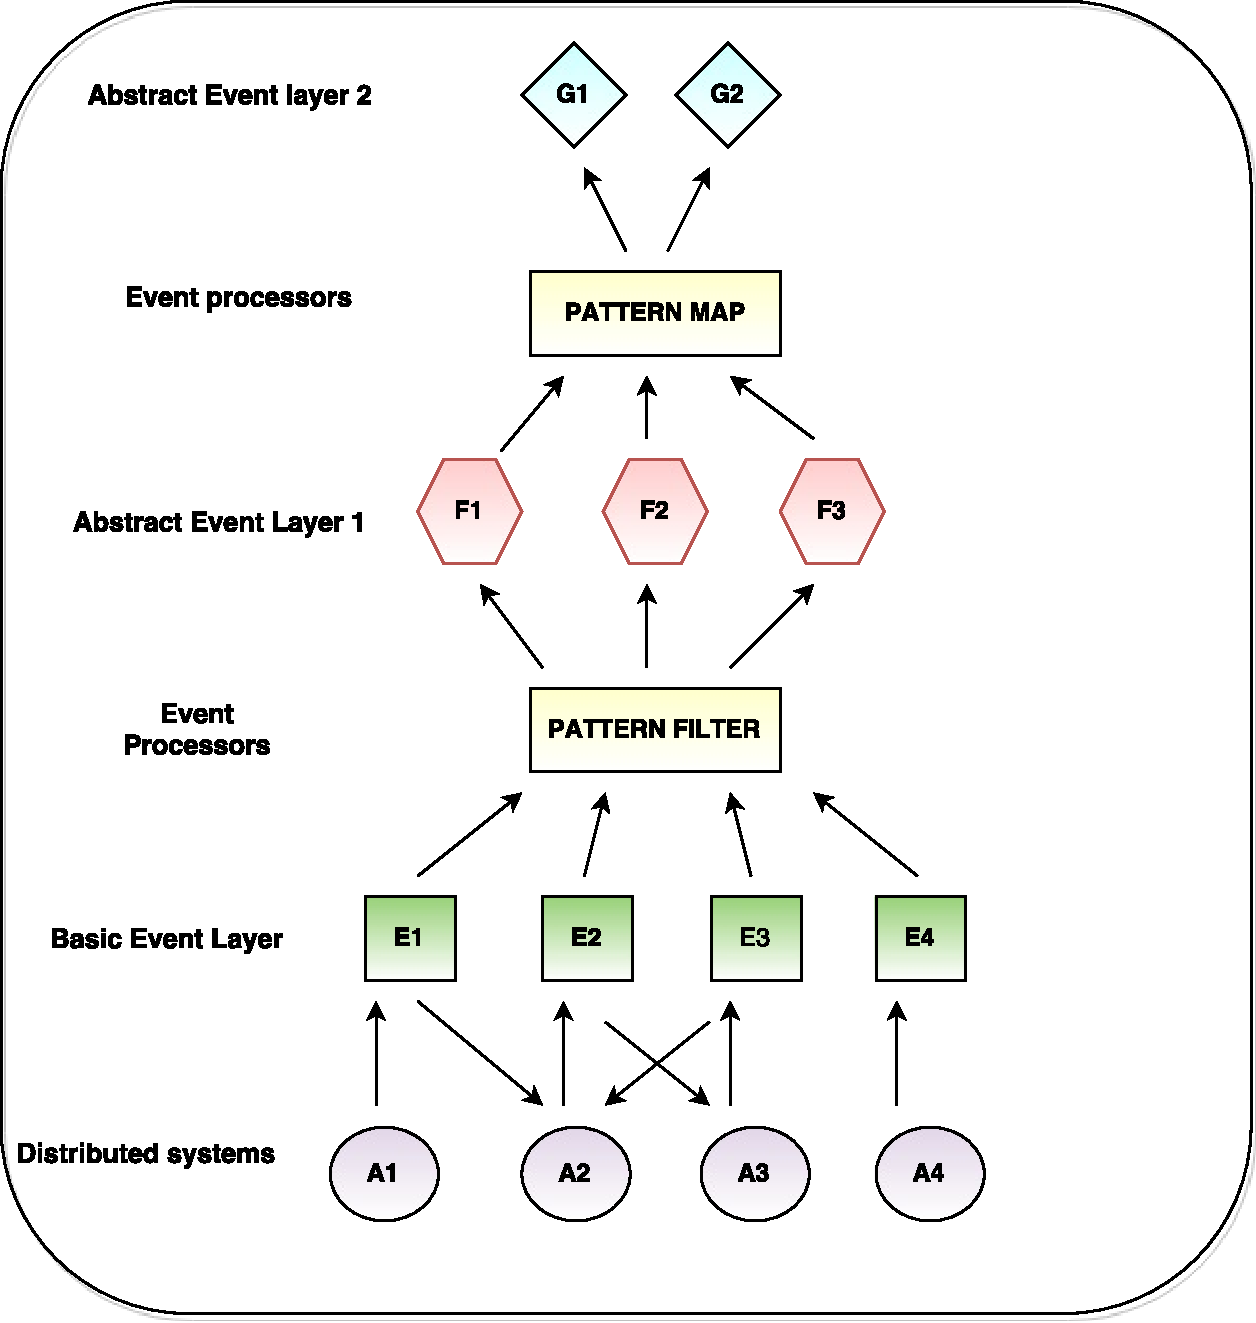
\includegraphics[height=10cm]{Luckham.pdf}
\end{figure}

\subsection{Hierarchical event abstraction}
Luckham et. al \cite{luckham1998complex} presents a hierarchical view of a complex event processing system based on a hierarchy of abstraction in events. As events move up the layer, they are subjected to different operations which transform the stream of events. At each layer of abstraction, the events may be delivered to interested sinks or sent to other compute nodes for further processing. A complex event processing system may thus be seen as series of operators applied to events depending on the desired event abstraction required by the consumers of events. Operator placement as such is a crucial research area in such systems. In section 3.1 a brief discussion is presented on the operator placement strategies within distributed complex event processing systems. 

\subsection{Communication models in complex event processing}
One of the most important traits of a complex event processing system is the decoupled nature of communication between the producer and consumer of events. 
\begin{itemize}
	\item Pub-Sub: In the publish-subscribe model of communication the senders of the message, otherwise called publishers, do not send the message to the receivers of the message, otherwise called subscribers. Rather the messages are published to a broker without the knowledge of the subscribers. The publishers advertise the topics to the broker and subscribers subscribe to a topic. A topic can have many publishers and many subscribers. On receiving a message on a topic, the brokers are responsible for delivering the message to the subscribers. Pub/Sub can be classified as a wide message delivery model of communication. Complex event processing systems are deployed using the pub-sub communication model for decoupled event delivery, where the consumers and producers of events are moving; with only the broker as a non-moving entity with compute nodes within complex event processing systems behaving both as producers and consumers of events. There are several Pub-Sub based notification services in the market today. Google Cloud Pub/Sub \cite{Krishnan2015} is one example of a thriving publish-subscribe message oriented middleware.
	
	\begin{figure}[H]
		\centering
		\caption{Publish-Subscribe communication model} 
		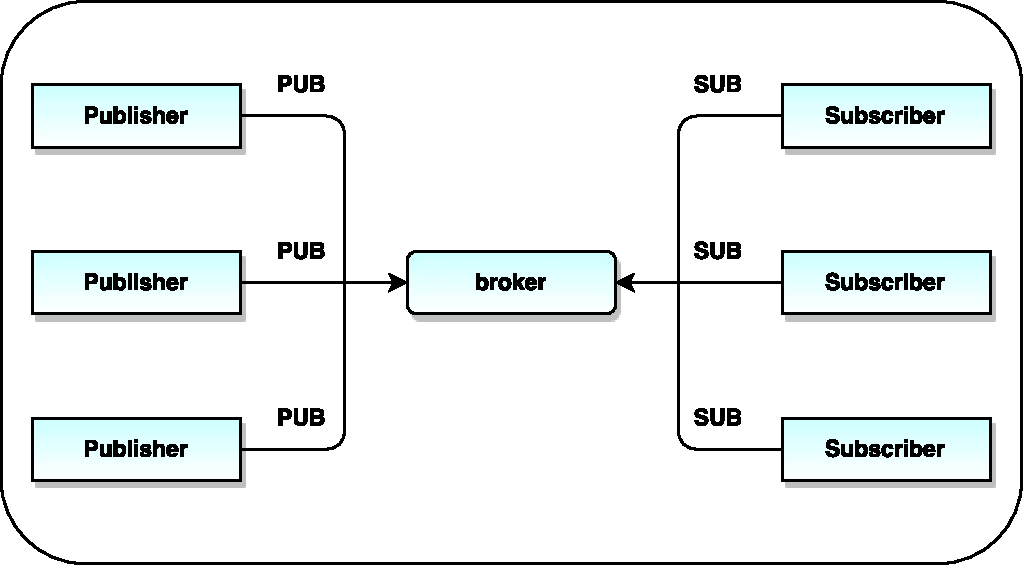
\includegraphics[height=6cm,width=12cm]{pubsub.pdf}
	\end{figure}
	\item Push-Pull: In a push-pull model of communication the messages are distributed to multiple workers who are registered as its pull clients. The pull clients which can do processing on their own do not rely on any broker but instead, have their pull clients to which the events are redirected. The extent of processing or filtering of events is directly dependent on the implementation. However, the events in this model of communication are sent evenly to multiple workers who may send the processed events to a single collector or different set of collectors create different stages of processing. The push-pull model is a pipe-lining pattern where all the subscribers need not receive the same message. Apache Kafka \cite{kafka2014high} is a high throughput distributed messaging system which uses the push-pull communication model to build robust data pipelines.
	
	\begin{figure}[H]
		\centering
		\caption{Push-Pull communication model} 
		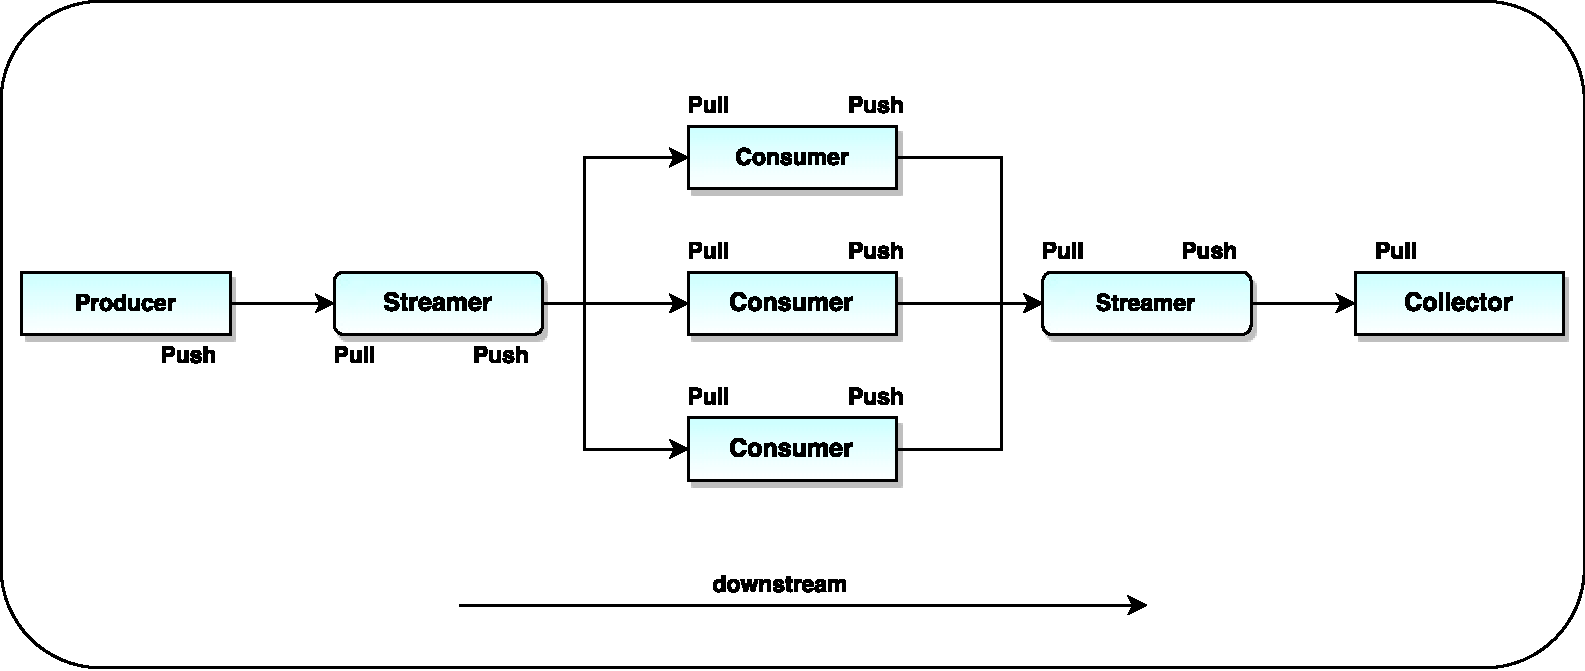
\includegraphics[height=8cm, width=16cm]{pushpull.pdf}
	\end{figure}
\end{itemize}


\subsection{Event Query languages}
Another crucial component of any complex event processing system is an event query language. Event query languages allow for the expression of user logic in a concise manner that is understood by the processing engine. Event query languages direct the processing engine to make sense of an event by describing the patterns for an event. Modern event query languages are equipped with capabilities to express temporal relationships among events with instructions for explicit and precise operations upon detection of events which share non-obvious relationships. Sophisticated features provided by modern event query languages include moving time windows, detection of causal relationships between events, aggregation of event data, generation of new events, etc. For example, Esper \cite{Esper} offers a domain specific language for dealing with high-frequency time-based events with SQL-like queries with support for sliding windows and event-series analysis.

\section{Software Defined Networking}
Software defined networking is a dynamic network programming paradigm that uses open interfaces to enable programmability of network devices. The primary focus is on aggregating the so-called control plane functionalities of all the network devices such as system configuration, management, and exchange of routing table information at a logically centralized location. The approach implies that the control path is decoupled from the fast path of the network device. While both the planes are set to evolve independently in a vendor agnostic manner, the fast path still utilizes the policy information made available by the control path to treat the packets both in the incoming and outgoing directions.\\\\The  figure 2.1 depicts a typical software defined network and provides the comparison with a legacy network. The devices in the traditional computer networks are comprised of both control plane and fast plane functionalities embedded into them directly as shown on the left-hand side of the diagram. Such devices lack the global network state information and require manual configuration during deployment. It also demands a certain mechanism to frequently propagate the routing information due to the distributed nature of the control plane.\\\\ The software defined network architecture, on the other hand, is built on top of the commercial off-the-shelf hardware components. The architecture is decomposed into three distinct layers of functionalities as shown on the right-hand side of the diagram.\\
\begin{itemize}
 \item Network infrastructure layer: It is the bottom most layer of the SDN ecosystem and contains the network devices themselves (both virtualized as well as physical devices) that are capable of switching/routing packets at line rate. They expose programmable interfaces to be leveraged by the upper layers of the SDN architecture.
 \item Controller layer: It is essentially the logically centralized control plane of the whole network infrastructure underneath. It forms the middle-ware of the SDN ecosystem and provides the necessary framework that binds the applications that require network services and the protocols that communicate with the network infrastructure. The vendor agnostic nature of the SDN architecture necessitates a set of communication mechanisms towards the network infrastructure which is commonly termed as southbound APIs. The OpenFlow, NETCONF, and OVSDB protocols are examples of such mechanisms provided by the SDN controller. 
 \item Application layer: The layer is composed of various network applications and the Northbound APIs exposed by the controller layer. Although there is no normative standard to describe what  Northbound APIs are comprised of, Restful APIs are prevalent in present day SDN applications. Some SDN controllers such as the OpenDayLight also provides OSGi based interfaces for native network application development.
\end{itemize}


\begin{figure}[H]
 \centering
 \caption{SDN Architecture}
 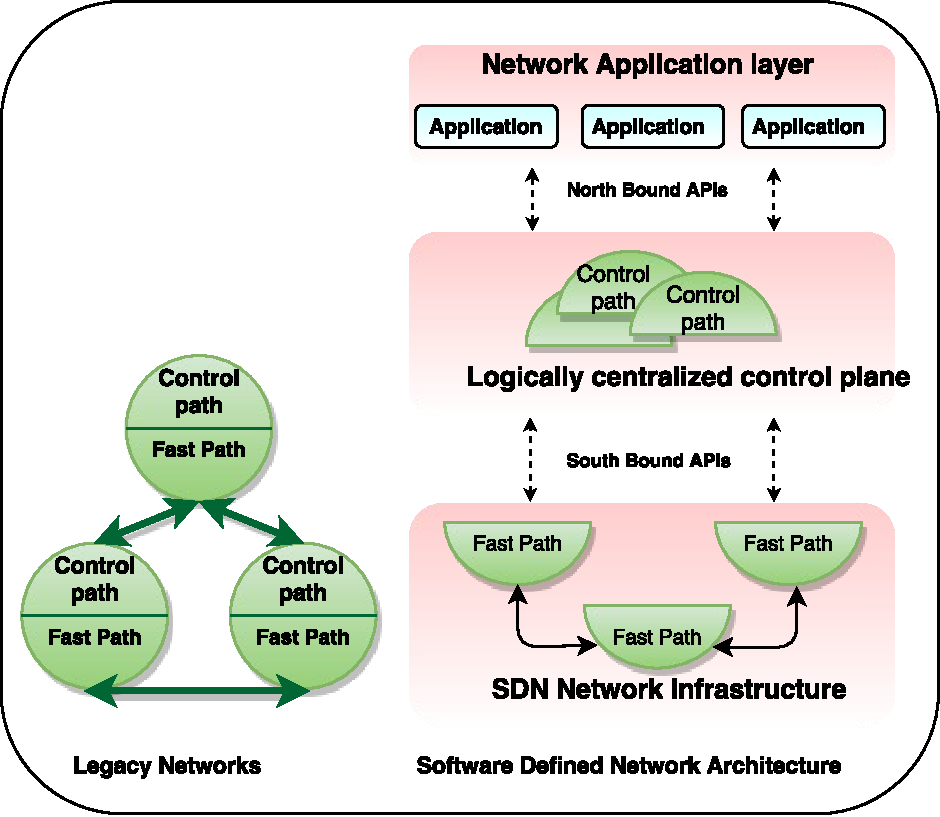
\includegraphics[height=9cm]{SDN-Architecture05.pdf}
\end{figure}

\section{OpenFlow}
The OpenFlow protocol is the default southbound API of choice in the SDN-enabled networks. Initially, it was considered as a communication mechanism that facilitates experimental protocols to be run in the computer networks \cite{OpenFlow-White-Paper}. It has now evolved into a rich set of APIs which can be leveraged to modify the forwarding behavior of network devices. The OpenFlow capable devices are manufactured from multiple vendors and include routers, switches, virtual switches, wireless access points\cite{OFArchive} and so on. \\\\To delve deep into the OpenFlow protocol features, the specification adheres to the SDN principle by separating control functions from the devices and thereby centrally managing the global forwarding policies in the network. The protocol has a set of messages defined for communication between the SDN controller and the underlying network. The OpenFlow capable switches operate based on the match-action policies programmed into their forwarding database. The match-action policies are defined on one or more flow-tables and a group table built into OpenFlow-capable switches. The flow-tables are essentially a set of rules containing packet headers/characteristics against which the packets in a flow are matched to make a packet modification/forwarding decision. The set of linked flow tables that provide matching, forwarding, and packet modification in an OpenFlow switch is termed as a pipeline \cite{OFSwitchSpecification} and hence the packets are said to undergo pipeline processing.  The pipeline processing of a packet may require that a packet traverses through one or all of the flow-tables defined in the incoming or outgoing direction. It should be noted that the packets are subjected to processing by a different set of flow-tables defined distinctly for ingress and egress directions. The SDN controller utilizes OpenFlow messages to add/modify/remove rules into and from the flow-tables.
The rules in a flow-table are assigned priorities to resolve match conflicts, and highest priority rule entry always takes effect, and the action(s) associated with the rule selected is executed. Besides actions, OpenFlow also allows several packet/byte level counters to be tagged along with a flow-rule. Such counters are useful in traffic monitoring, shaping and policing activities. The protocol, for the purpose mentioned above, also allows the SDN controller to describe a meter table with per flow meter entries (associated with flow rule entries) to achieve traffic shaping and policing. \\\\ Further, to provide an overview of the OpenFlow protocol communication mechanism, it supports three different type of messages:
\begin{itemize}
 \item Controller-to-switch: These messages are used to manage and obtain the status of the switches. For example, the controller can request a switch for its basic capabilities using the Features message.\\
 \item Asynchronous messages: These kinds of messages are triggered by the switches to inform the controller about change in operational status or other network events. For example, PACKET\_IN message is triggered to indicate a packet arrival event.\\
 \item Symmetric messages: These messages are typically heartbeat messages, error messages or initial Hello messages initiated by either of the parties i.e. the SDN controller or the network device. Some experimenter messages may also fall under this category.
\end{itemize}A detailed description of all the messages and their implied functionalities can be obtained from the OpenFlow specification document\cite{OFSwitchSpecification}. The OpenFlow protocol provides reliable message delivery through its channel connection built on top of TLS or simple TCP. The standard does not automatically impose any acknowledgments for the messages sent nor does it ensure ordered processing of messages and is left open for the switch implementations to handle the same.

\section{RYU SDN Controller}
SDN controller is the brain of the SDN ecosystem with all the network-wide control functions aggregated at the controller as a global snapshot which is then presented as a single logical switch to the application domain.  There have been several implementations of the controller since the inception of the SDN. Some of the salient features of an SDN controller include the ability to scale out the network without bounds, the ability to support network programming in a vendor agnostic manner, protocol agnostic characteristic that allows the design and use of new southbound APIs and so on.  Some of the open-sourced, adopted controllers are OpenDayLight, ONOS, Floodlight, RYU. As part of the thesis work, RYU is chosen as the controller for programming the Open vSwitch. RYU follows a simple modular design wherein applications are built and deployed as single threaded Python processes leveraging RYU's event based mechanism to interact with the other SDN applications. RYU also supports OpenFlow protocol along with various other southbound APIs which renders it just sufficient to extend the protocols, develop and deploy the desired controller application for this thesis work with a shorter development life cycle.\\\\RYU SDN controller at its core contains a set of components with well-defined APIs. The base component is the app\\manager which takes up the responsibilities such as loading RYU applications, providing contexts to RYU applications and routing messages between RYU applications. It has a dedicated OpenFlow controller component to handle protocol connections to the switches. The component also generates appropriate OpenFlow events to be handled by RYU applications. The other critical component of the controller is the RYU OpenFlow wire protocol encoder and decoder \cite{RYU-Documentation}.\\\\Each RYU application is equipped with its own FIFO message queue to receive events that are processed in the order of arrival. Although the application itself is expected to be developed as a single threaded module, RYU internally spawns a thread to handle events per application module. RYU provides another way to communicate with other applications/components by exchanging contexts which are essentially application specific python objects. Since the controller is built around event-based components, RYU applications naturally are equipped to observe and generate events. An application can observe/listen to events by using a specific python decorator exposed for event handling.\\\\ As part of the work, the OpenFlow protocol's match-action capability is extended to support event types and attributes. Through this mechanism, SDN controller facilitates the switches to detect events based on the event rules. The RYU controller like its counterparts also can provide Restful API support to network applications. The application developed hence exposes the Restful APIs to commission event-based rules on Open vSwitch.


\section{Intel Data Plane Development Kit}
Intel Data Plane Development Kit (DPDK) \cite{DPDK} is set of data plane libraries and userspace drivers that enable fast packet processing. Intel DPDK runs in Linux userspace and thus allows application programs to bypass the kernel for packet processing. As a consequence users of the DPDK libraries have the flexibility to run third-party fast path network stacks and develop fast packet capture algorithms all in the userspace. By enabling kernel bypass, DPDK reduces the number of cycles taken to send and receive packets. The main components of DPDK, as illustrated in the figure  are:

 \begin{figure}[H]
 \centering
 \caption{DPDK Components}
 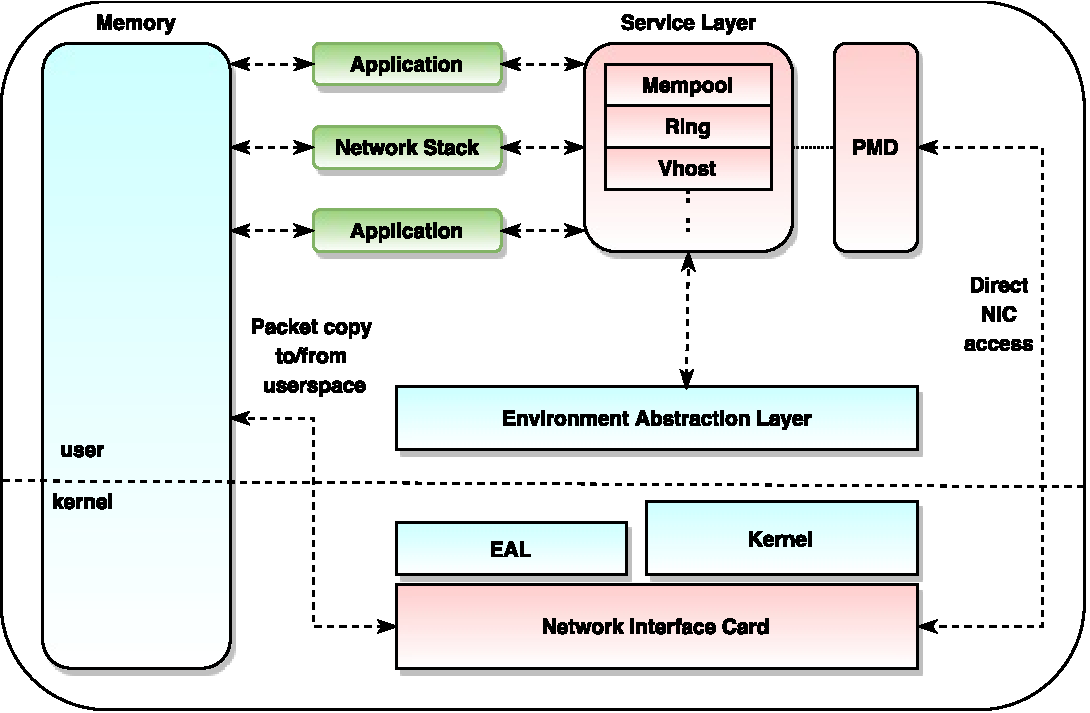
\includegraphics[height=8cm]{DPDK03.pdf}
\end{figure}

\begin{itemize}
 \item Environment Abstraction Layer: The \ac{eal} provides an interface for the DPDK applications and libraries to access resources such as memory and hardware. The libraries and the applications are not aware of the allocation of these resources. The EAL is responsible for physical memory allocation, multi-process support, Interrupt-handling, PCI access, CPU feature recognition and core affinity setting among others.
 \item Service Layer: The service layer of DPDK consists of various libraries to enable DPDK applications to make use of the features provided by the EAL. The service layer can be seen as the provider of 'system calls' to the DPDK applications. For example, the ring library provides a lockless FIFO ring implementation for Rx and Tx queues with support for burst queue and dequeue; The Mempool library implements a pool-based aligned memory allocator with features such as per-core cache and hugepages; The vhost library provides a userspace virtio driver that allows the users to manipulate the vring. Full list of DPDK libraries can be found at \cite{DPDK}
 \item Poll Mode Drivers: The DPDK \ac{pmd} provide userspace device drivers and APIS to set up queues and devices. The PMD is capable of accessing the transmit and receive queues directly without interrupts by continual polling. This ensures that the packets at the receive queues are directly received by the userspace application when receiving, and the packets from the user space are directly at transmit queues when sending.
\end{itemize}

\subsection{DPDK Vhost library}
The DPDK vhost library requires a special mention because of its support for vSwitch implementations. The vhost library provides a userspace vhost driver to manage vhost threads for corresponding virtio front-end devices in a guest. Before understanding the DPDK vhost library, it would be useful to understand the vhost-net acceleration standard on virtio. As illustrated in figure 1.1 in section 1.1, the QEMU userspace process normally provides the virtio back-end implementation for the virtio-net front-end device in a guest. This results in a situation where QEMU is involved intensely in the packet I/O thereby increasing the context switch required. As an improvement to this virtio standard of having a front-end in guest and back-end in QEMU, the vhost-net standard came into being. In the vhost-net implementation, a vhost-net device is introduced into the kernel space which acts as the back-end to the virtio front-end device in the guest. Keeping the vhost-net device in kernel ensures that QEMU process in not needed for every packet transfer between the host and guest. Instead, QEMU is involved in setting up the event file descriptors and the Interrupt file descriptors. Vhost creates an individual thread per virtio device which waits on the eventfd provided by QEMU. The host machine uses the eventfd to communicate with the guest by binding the eventfd to an interrupt source or listening to the eventfd which is triggered by the KVM when the guest writes the NOTIFY register. 

 \begin{figure}[H]
 \centering
 \caption{Vhost-net acceleration}
 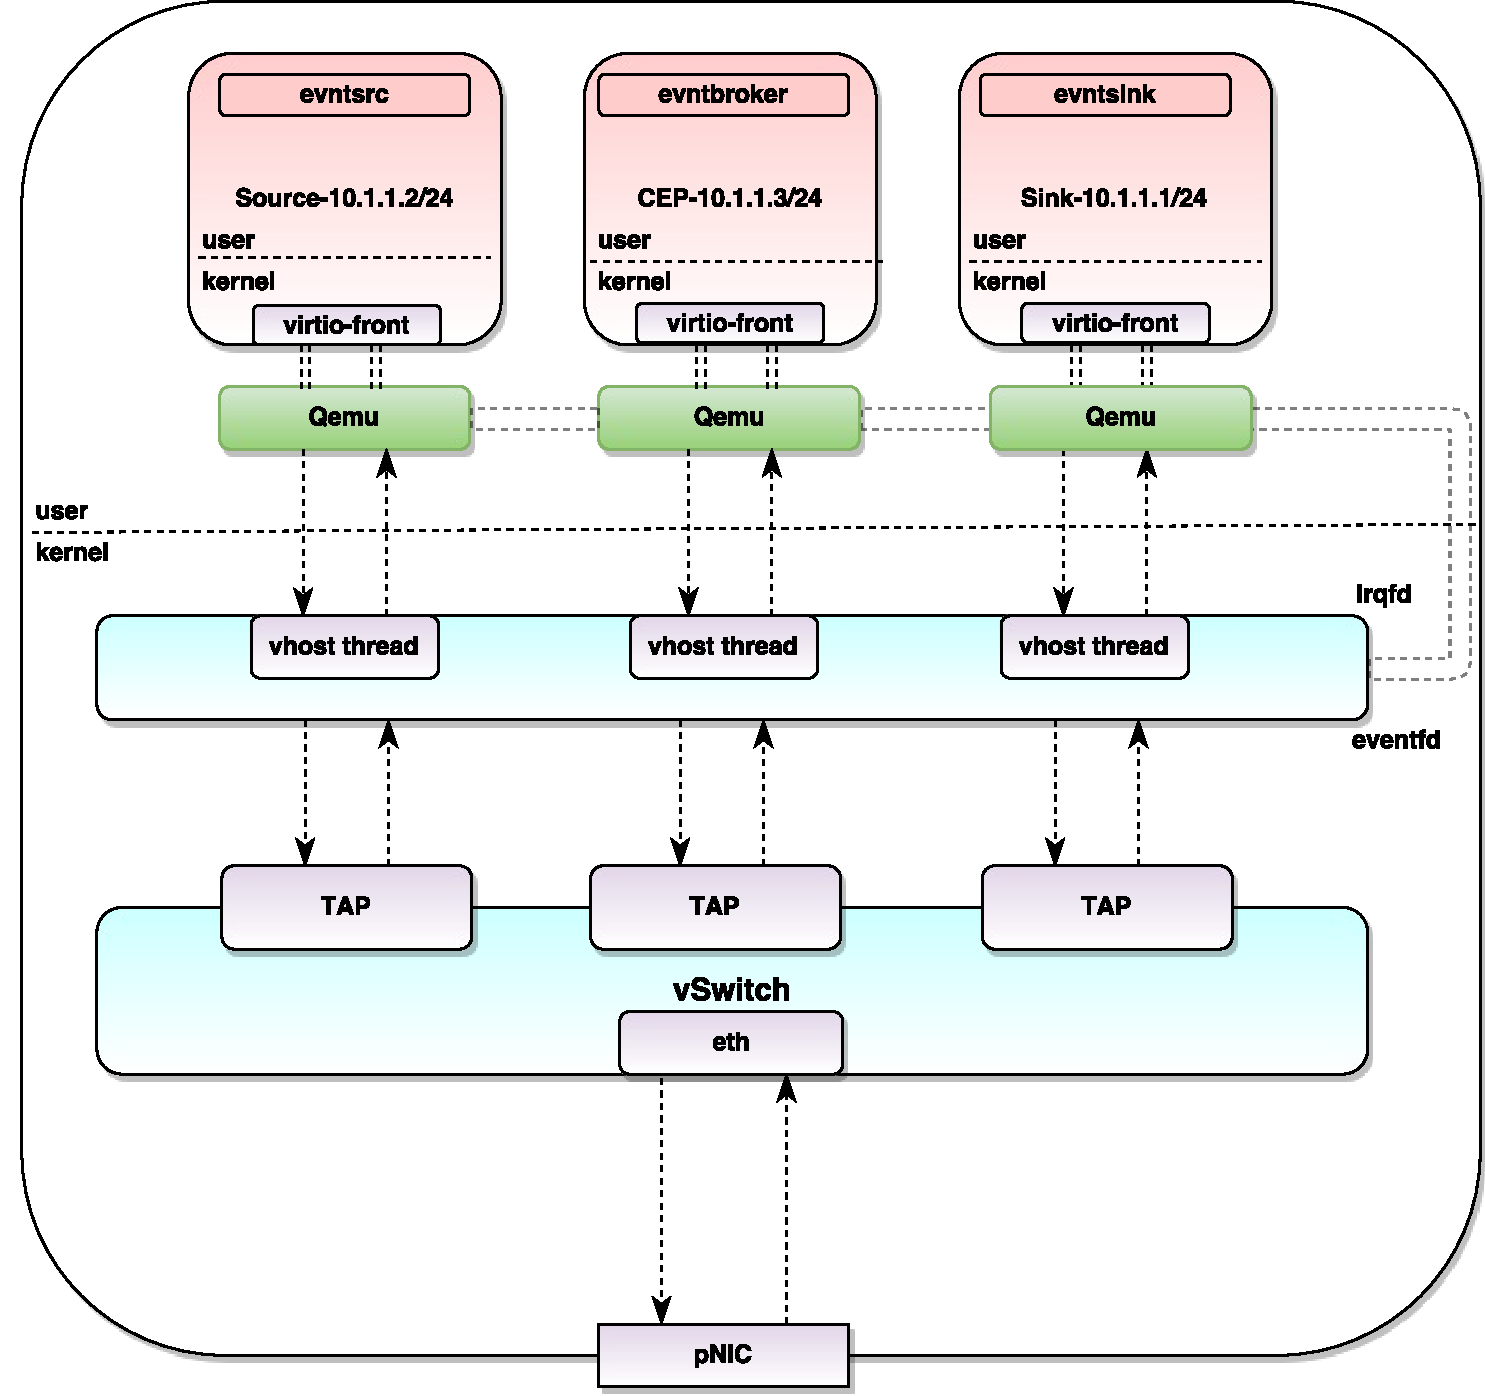
\includegraphics[height=10cm]{vhostnet.pdf}
\end{figure}

As illustrated in figure 2.5, vhost-net acceleration relies on QEMU for device feature negotiation, migration, etc. The vhost driver at the kernel is not a full-fledged virtio device implementation because QEMU still controls some parts of the setup. However, a virtqueue exists between the virtio-front end in the guest and QEMU. The vhost thread in the kernel can \ac{dma} to and from the virtqueue giving it access to the virtio-front end without QEMU intervention. This implementation can be contrasted with the DPDK vhost implementation which is illustrated in figure 5.13. In the DPDK vhost implementation, the vhost driver is moved completely to userspace. A dpdkvhostuser port attached to the vSwitch registers callbacks to the vhost library in userspace, which is called when the vhost device is activated/deactivated in the guest. For each virtio device in the guest, a vhost device is created by the vhost driver(vhost library). The dpdkvhostuser port (vhost-device) and the virtio device share a virtqueue that enables them to exchange packets without intervention from userspace QEMU directly. So a packet at the physical NIC is lifted into the userspace vSwitch where it is switched to the dpdkvhostuser port attached to the guest VM. Since the dpdkvhostuser port shares a virtqueue with the virtio device in the guest, the guest receives the packet with minimum overhead.

	\chapter{Related Work}
There has been a great deal of research in the areas of Complex Event Processing, Software Defined Networks, and High Performance packet processing. Since this thesis derives motivation from all the three, related work is surveyed and organized according to the domain. In this chapter, the outcomes of the research works and takeaways from the perspective of the thesis are briefly discussed to give thee rational or motivation behind the implementation of the thesis.

\section{Deployment Strategies and Operator Placement in Event Processing}
Since the thesis focuses upon creating a data plane solution specifically tuned for the Event Processing/Event-Based systems, it is important that key factors impacting the design of such systems are studied in detail.
Cugola et. al \cite{Cugola} discuss different deployment strategies for distributed complex event processing systems. The strategies described in the paper can be classified based on:
\begin{itemize}
	\item \textbf{Organizing processors into processing trees}: Primitive events from sources are collected, filtered, and processed as the move upwards in the tree. This allows for incremental evaluation at intermediate processors in a manner similar to staged processing. 
	\item \textbf{Forwarding advertisements to processors}: Each processor in the processing tree maintains an advertisement and subscription table.  When receiving an event notification, each processor computes the set of subscription that match the event and determine which node in the processing tree receives it. 
	\item \textbf{Rule deployment}: The rules are recursively partitioned into partial rules and deployed in the root to source of the processing tree. 
	\item \textbf{Notification Forwarding}: Two concepts of event forwarding are discussed - Push based and Pull based. In Push based forwarding, a processor forwards all matched primitive events to the parent; whereas in Pull based forwarding the processor stores the matched event until it is explicitly asked by the parent. 
\end{itemize}
In addition to deployment strategies, Cugola et. al present an analysis of content-based filtering of primitive events. Their analysis highlights the advantage of content-based filtering close to source to reduce the network traffic in both distributed and centralized deployment. Their work informs and motivates the thesis at many levels. With a content-aware switch and a SDN based controller to deploy rules, a logical processing tree based on event types can be constructed to process different event types at different processors.  Since the controller has a logical view of the network, rules can be deployed in such a way that one processing node is responsible for a pre-decided event types. The events from one processing node can be then chained to another based on the logical processing tree using a push based forwarding strategy.\newline 

Pietzuch et. al \cite{pietzuch2006network} discuss the NP-hardness of the operator placement problem and propose a heuristics based approach. They propose a stream based overlay network in between the physical network and the stream processing system and delineate three challenges in the operator placement problem: a) Achieving good application query performance b) Use network efficiently c) Reuse existing operators when appropriate. Zhou et. al \cite{zhou2006efficient} present a cost model for dynamic load balancing in distributed stream processing systems and identify the importance of load balancing in streaming applications. While publications such as \cite{backman2012managing} and \cite{chatzistergiou2014fast} focus on reducing the end to end latency, \cite{aniello2013adaptive} and \cite{cui2016big} focus on reducing the inter-node traffic, and \cite{rizou2010solving}, \cite{pietzuch2006network} focus on reducing the overall network usage. While all the concerns are valid for the distributed event processing environment, the research focuses using the application layer for optimization. Even when an In-Network solution is discussed, the solution is based on deploying processing nodes as close to the data source as possible. The discussed research works provide good  motivation for selecting optimization parameters in Event Processing systems, however the solution provided in the thesis is a pure data-plane solution, focusing utilizing the underlying network service instead of the application level processing node.


\section{Fog Computing and Software Defined Internet of Things}
There has been an exponential growth of connected devices, and it is unanimously accepted that the number of connected devices is only going to increase from the current 10 billion nodes to 50 billion nodes over the next few years. This presents us with two interesting challenges: 
\begin{itemize}
\item \textbf{Handling massive streams of data from the sensory nodes}: Large cloud deployments of today are built to handle massive amounts of data from web and other batch processing applications. But when there are billions of sensory nodes located in widespread geographic location producing streams of sensor data, transporting all the data to the cloud is counter intuitive. For one, it creates unnecessary traffic in the network because most of the sensing data is discarded anyway and for another it creates a lot of latency. And as properties of sensory data goes, it is mostly useless; but when it is not, it is most likely very important. This problem has been discussed even before the explosion of IoT networks. The operator placement problem discussed in the previous section to some extent attempts to address this problem by moving the operators closer to the sources of data in order to react to events faster and reduce network traffic. Fog computing is a local cloud deployment paradigm which does exactly this. Bonomi et. al \cite{bonomi2012fog} discuss in detail the characteristics of IoT and advantages of Fog deployment in IoT. 
\item \textbf{Maintaining the massive network for the sensory nodes}: As billions of wired and wireless sensory nodes join the network, traditional networking is insufficient to utilize the paradigm fully. Software Defined Networking which we discussed in Chapter 2.2, introduces significant flexibility for resource management by separating the data plane from a software based control plane. Software Defined Internet of Things promises an architecture to seamless manage, configure, and spawn billions of sensory nodes to create Sensing-as-a-Service(SaaS) paradigm. Research done in \cite{el2015software} , \cite{qin2014software} and \cite{flauzac2015sdn} detail such an architecture and provide prototype deployments with network models.
\end{itemize}	
Truong et. al \cite{truong2015software} deploy a Software defined Fog computing Adhoc vehicular network, whereas Xu et. al \cite{xu2016towards}  prototype a Software Defined Fog computing Message Queueing Telemetry Transport (MQTT) broker for IoT devices. Prototypes built by \cite{xu2016towards} and \cite{flauzac2015sdn} deploy Open vSwitch as the Openflow switch in their respective SDN based Fog deployments. This highlights the versatility of Open vSwitch in both large scale global cloud and small scale local Fog deployments. These works motivate the selection of Open vSwitch for an application aware deployment in cloud, be it in large data centres or in IoT networks.

\section{Application-aware Data Plane Processing in SDN}
Mekky et. al \cite{mekky2014application} prototype an Application-aware implementation of Open vSwitch(OVS). The prototype implementation, as shown in the figure 3.1 - sourced and reinterpreted from \cite{mekky2014application} -  creates a separate application module within the Open v Switch with  its own separate app-table. The app-table is staged after the Openflow flow table pipeline. The application module is responsible for handling the flow out of the app-table and executing app-actions. An app-action is capable of doing the following operations:
\begin{itemize}
\item Determine actions for a packet and modify the state if required.
\item Generate or modify the rule set for processing this flow.
\item Remove flows from the Openflow tables and generate packet out to other switches.
\item Send custom vendor messages to controller.
\end{itemize}
A table-miss in the standard Openflow table is sent to the app-table instead of the controller as in the standard Open vSwitch. The app-table is configurable with custom app-actions. These app-actions are executed within the application module in the userspace. In summary, the application module within the OVS runtime, behaves like a light-weight controller capable of receiving select flow, executing them in userspace, and taking decisions by calling the Openflow APIs. The research work also provides valuable information about the interception of packets within the OVS as a design choice. Mekky et. al lay out three options to the said end:
\begin{itemize}
	\item Intercept the messages between controller and OVS at the connection manager.
	\item Intercept the packet after looking up the Openflow flow table.
	\item Add app-actions directly to flow table and apply actions directly when the rule is matched.
\end{itemize}
 Although L4-L7 match is supported in the application module, the implementation does not scale to Event Processing paradigms where event patterns can occur in any packet of the stream. In such a scenario, the prototype implementation lifts each packet to the application module and out of the Openflow processing pipeline inducing processing latencies. This work provides motivation to keep processing in-line for scenarios such as stream processing where rules have to be applied for each packet in the stream.


 \begin{figure}[H]
	\centering
	\caption{Application Aware Data Plane Processing}	
	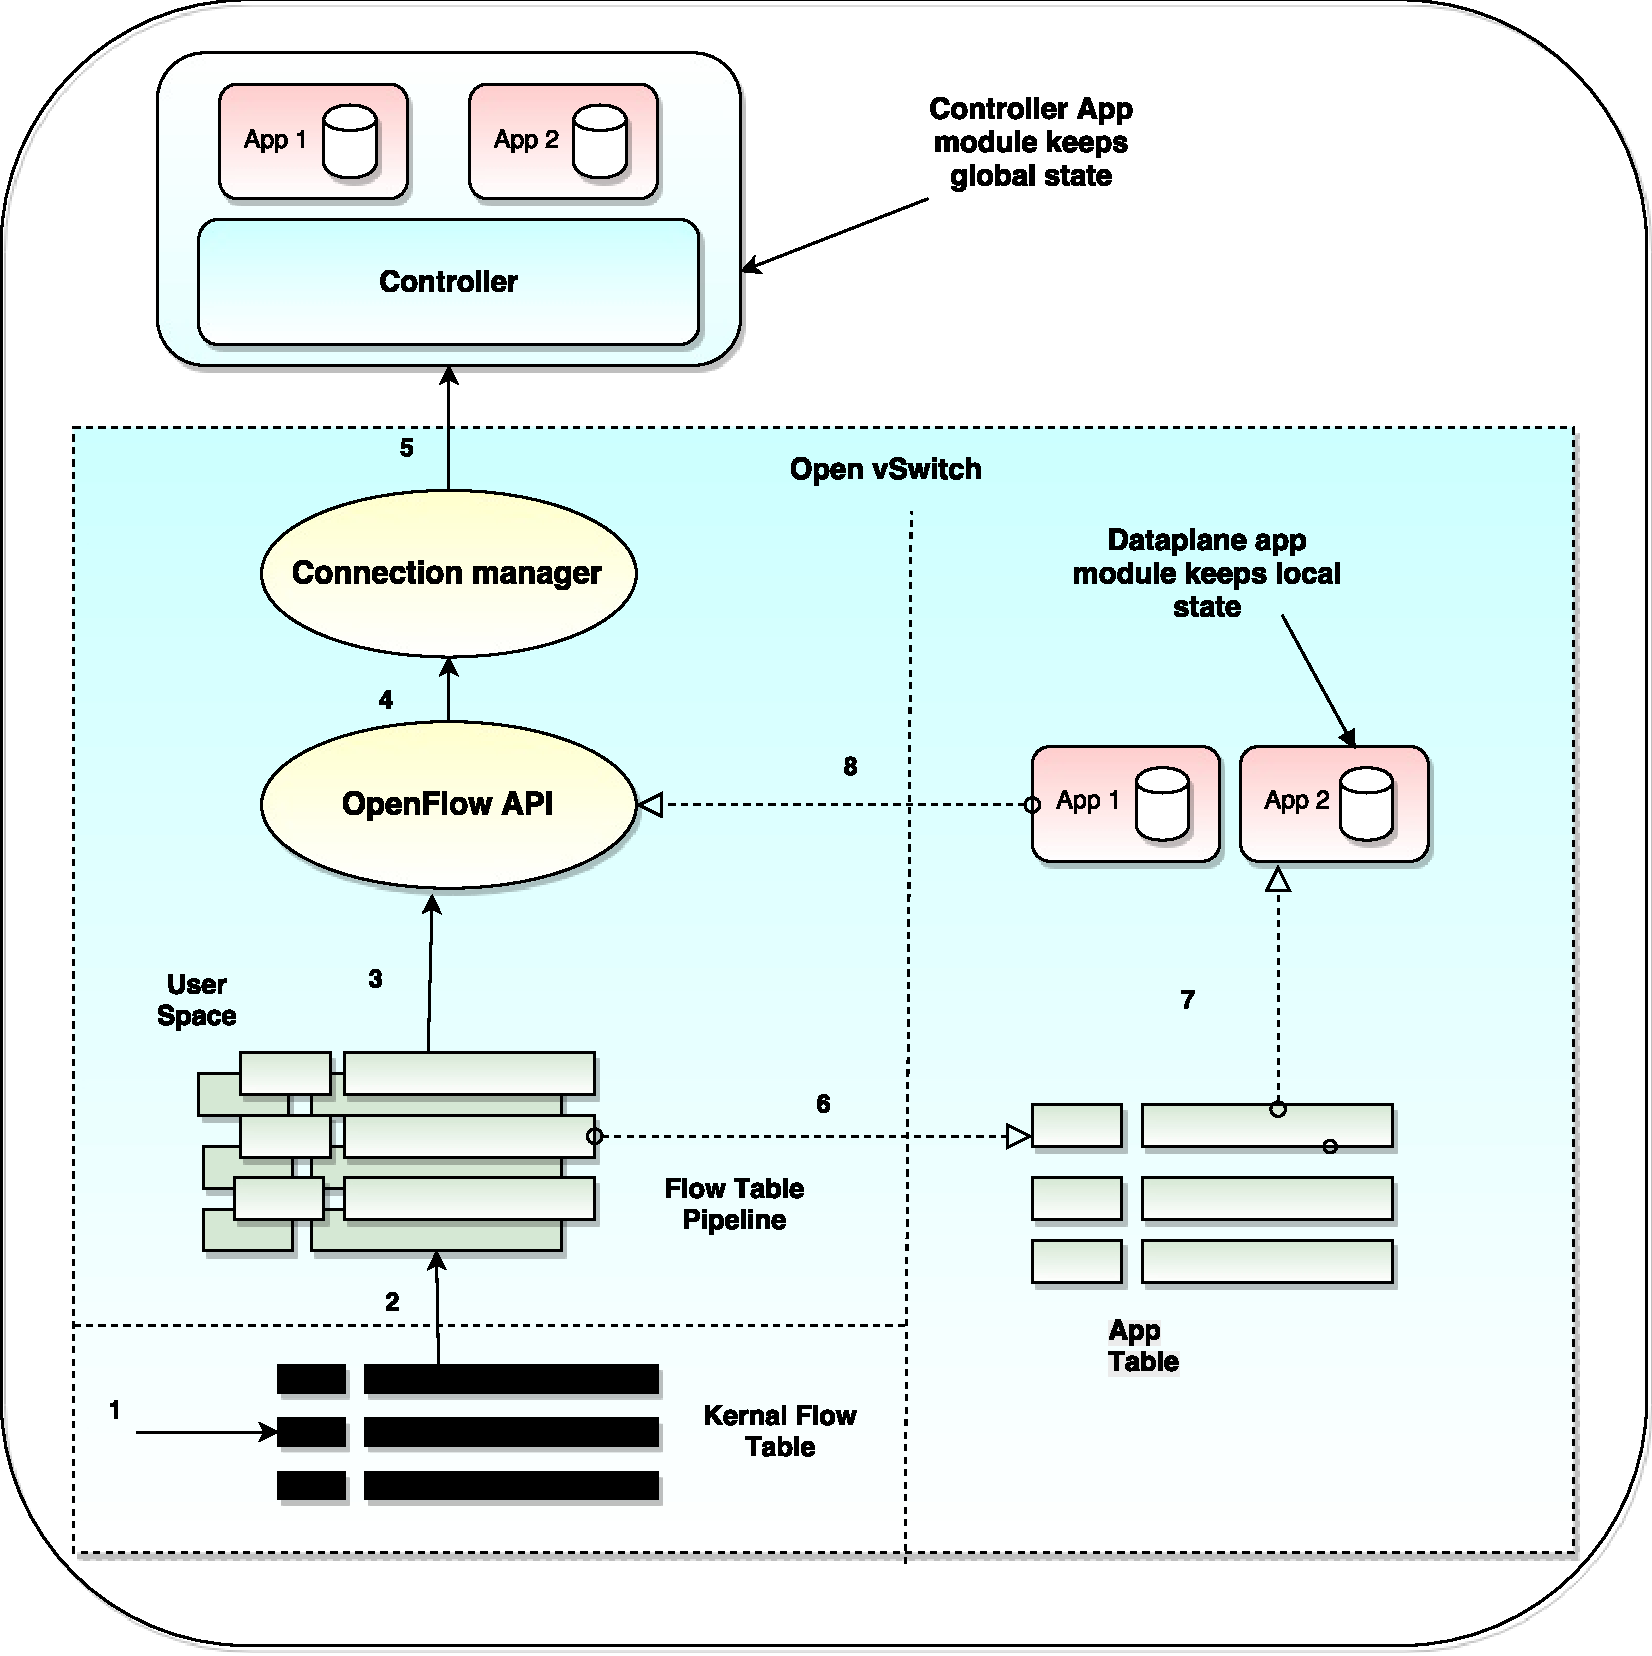
\includegraphics[height=10cm,width=13cm]{appaware01.pdf}	
\end{figure}


\section{In-Net: In-Networking Processing for the Masses}
Stoenescu et. al \cite{NpForMasses} prototype a ClickOS based \cite{martins2014clickos} processing platform running on commodity servers. Their results promise the possibilities of running single, in-expensive commodity servers scattered around in the network with the vision of providing a controller-based access to both network-providers and end users. The processing platform, which relies on ClickOS is capable of hosting upwards of thousand clients per box. In this model, end-users can demand for adhoc network service, in the box which can be provisioned instantaneously. While they also provide various security configurations and static analysis as a way to measure the validity of the provided service, the deployment model used provides a very interesting insight into the motivation for work done in the thesis. 
In the work done by Martins et. al on ClickOS, they consider two options to for the ClickOS switch

\begin{itemize}
	\item \textbf{VALE based deployment}: The first model uses a modified VALE \cite{Rizzo:2012:VSE:2413176.2413185}, a Virtual Local Ethernet switch to connect the virtual machines. VALE is a software switch which uses netmap (Discussed in Section 2) API and batched packet processing for high performance switching between guest virtual machines machines.
	\item \textbf{Open vSwitch}: The second model uses a standard Open vSwtich for connecting the guest virtual machines.
\end{itemize}

The results produced express that the performance of the modified VALE switch is better than that of the standard Open vSwitch; explained partly by VALE's usage of the netmap API - which allows the packet buffers to be mapped to the VM's memory space - and other modified APIs enabling batched packet processing.

 \begin{figure}[H]
	\centering
	\caption{In-Network processing model}	
	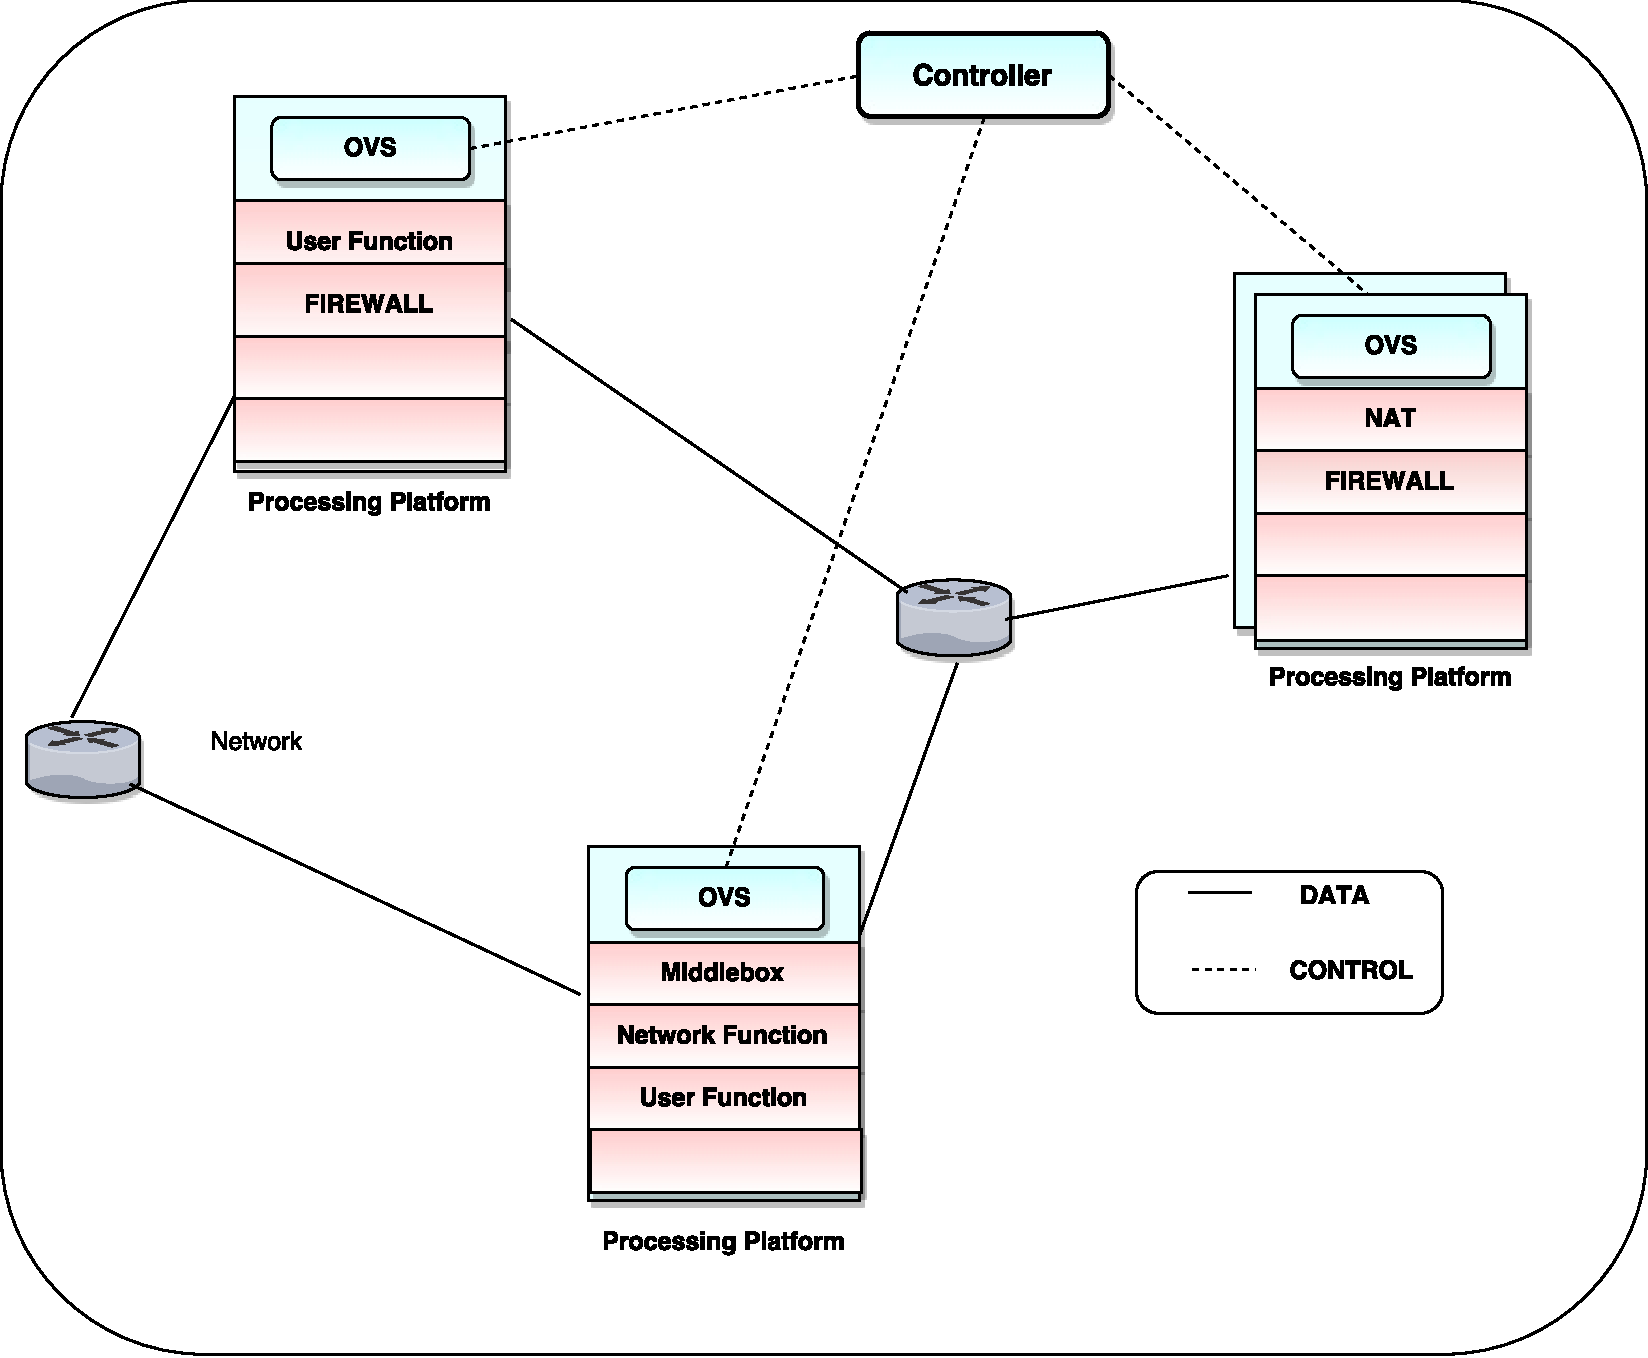
\includegraphics[height=10cm]{innet01.pdf}	
\end{figure}

However the implementation by Stoenescu et. al \cite{NpForMasses} uses the Open vSwitch within their processing platform, highlighting the versatility of Open vSwitch. The ability of the Open vSwitch to speak Openflow and thereby be configured by controllers in the Software Defined Networking model makes it a valuable option for deployment in In-Networking processing scenarios. One such deployment scenario is detailed in the figure 3.2 - sourced and reinterpreted from \cite{NpForMasses}. As we can see, the processing platforms are dispersed all around the network. Each processing platform consists of a Open vSwtich which is capable of speaking Openflow. The users and network operators rely on the Openflow controller to request, provision or service network functions. Although the performance of Open vSwitch does not compare well to that of a hardware unit, its versatility makes it a great design choice. Moreover with the advent of DPDK, the performance of Open vSwith can be vastly improved, all the more consolidating Open vSwitch as a design choice for the implementation in the thesis.

\section{SmartSwitch: Bluring the Line Between Network Infrastructure and Cloud Applications}
Wei Zhang et. al \cite{zhang2014smartswitch} prototype an application-aware networking platform that performs functions that are characteristically performed by compute platforms. They explore how the boundaries between applications and network infrastructure can be obscured by modern day packet-processing technologies.  They prototype a memcache-aware switch, that achieves application level redirection to memcached servers and local caching to allow immediate responses to hot requests. The paper examines three areas as use cases for their effort:
\begin{itemize}

	\item  \textbf{Load balancing}: Although SDN allows for a much more flexible policy shaping of the data plane, it still does not allow decision making based on data plane information. The packets still have to be send to load balancers and proxies for content based routing. An application aware  implementation may try to overcome this problem by enabling the software switch to perform redirection based on the application data.
.
	\item  \textbf{Storing Data within the network}: Focusing on content centric networks where forwarding requests and responses are based on names rather than location, an application aware switch may be equipped with a Hadoop-aware implementation and populated with cache keys and respective names for the keys. Doing so allows allows the switch to direct requests to nearest cache locations.

	\item  \textbf{Computation in the network}: When application data has to traverse through multiple Wide Area Networks, Wei Zhang et. al propose that it is more intelligent to process or store only the information that is relevant for the application. To this end they discuss the ability to deploy computation within the network to process and filter the data instead of blind routing/forwarding at the network. They contrast this with providing hardware based switching which incurs high cost and is not flexible to changing demands of the application.

\end{itemize}
The Smartswitch prototype is implemented along the above lines and is evaluated against Twitter’s TwemProxy server. Initial evaluation results show that the Smartswitch significantly reduces the latency for cached data. The work done in this paper provides motivation to continue exploring the possibilities to offload application context into the network and possibly tune the network services for specific applications. With the advent of Network Functions Virtualization and the resulting adhoc provisioning of network services in the network pipeline, this paper provides invaluable direction for the thesis. 

\section{NetVM: High Performance and Flexible Network Virtualization}
Hwang et. al \cite{hwang2015netvm} present a high speed network virtualization platform which promises line speed performance for high bandwidth network functions. They innovate on top of the Linux KVM and Intel DPDK platforms to provide:
\begin{itemize}
	\item A virtualization platform for network service provisioning which can perform at the level of custom hardware packet processing.
	\item A zero-copy delivery mechanism between VM's via their shared-memory framework.
	\item A hypervisor switch for intelligent load balancing via state-dependent or data-dependent approach.
	\item An architecture which enables the compositing of complex network services on multiple VMs.
	\item Security domains that differentiate between trusted and untrusted VM's for packet processing.
\end{itemize}

 \begin{figure}[H]
	\centering
	\caption{NetVM}	
	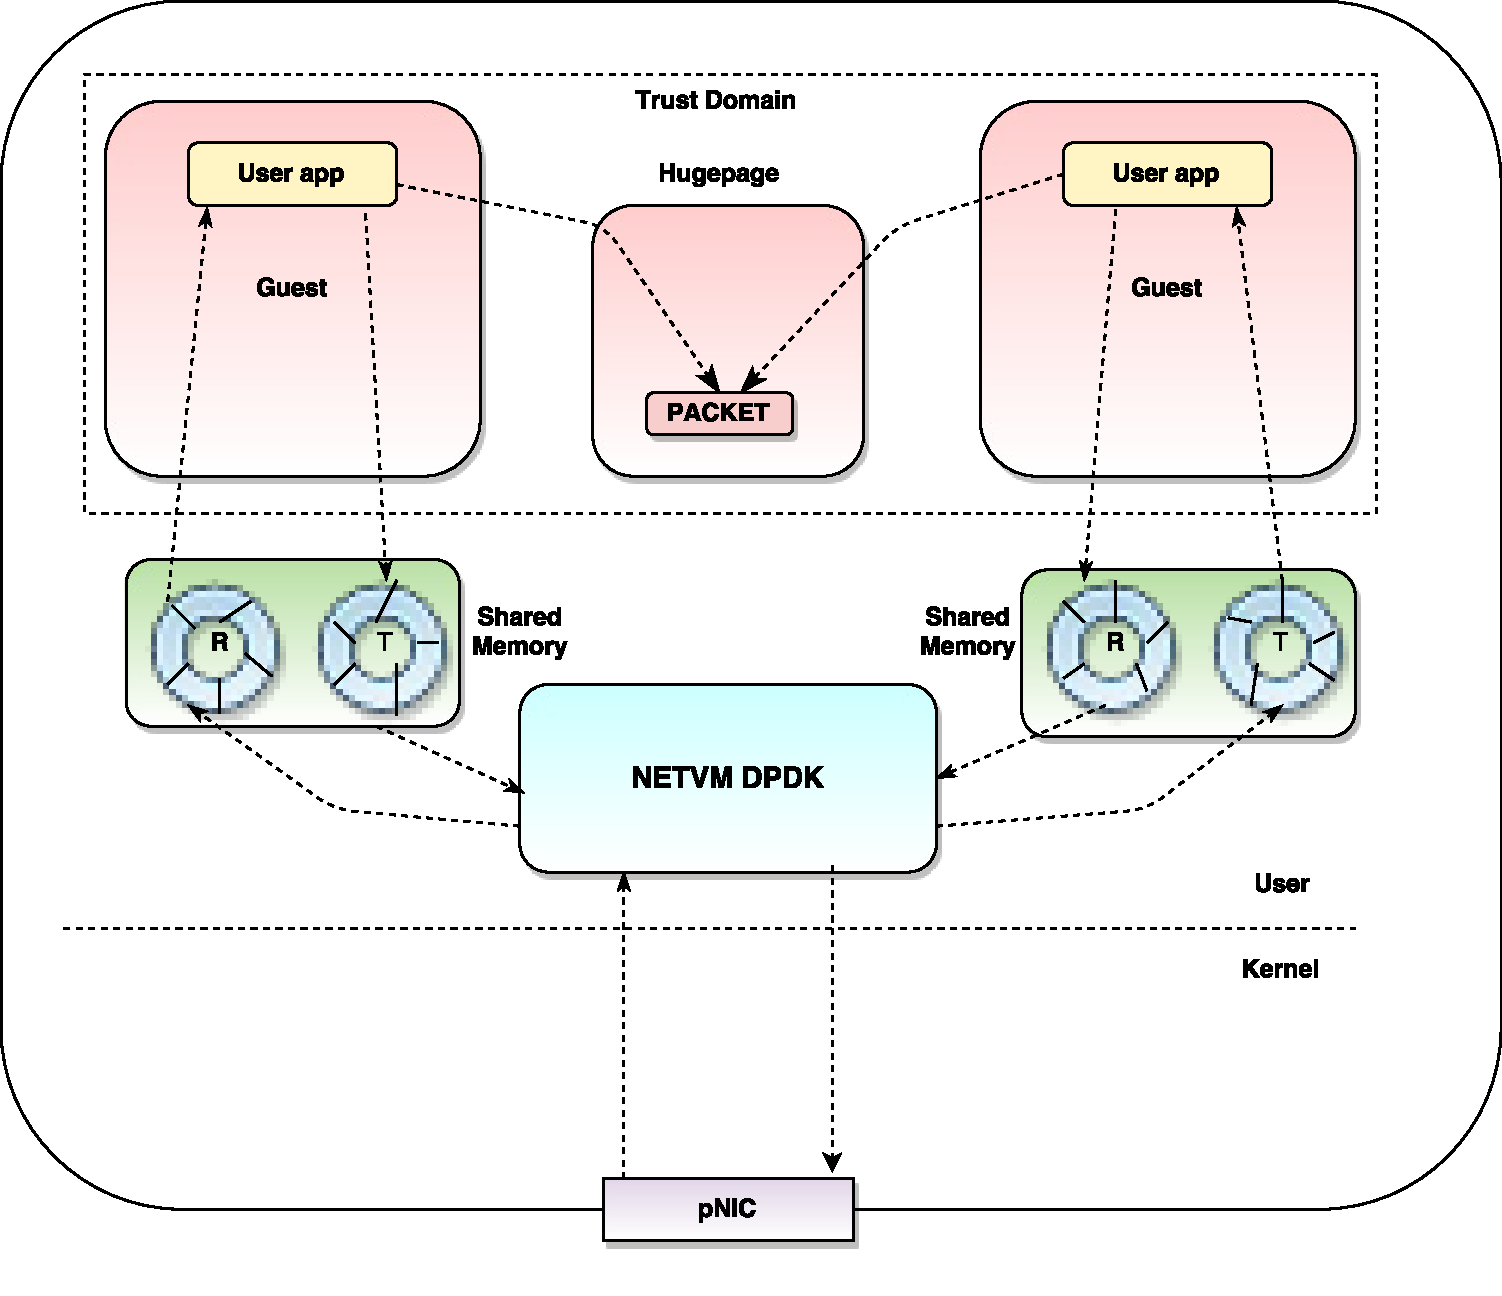
\includegraphics[height=10cm]{netvm01.pdf}	
\end{figure}

\subsection*{Zero-Copy Packet Delivery}
NetVM implements a Hypervisor switch, accelerated by the DPDK library. The implementation leverages DPDK huge pages support (discussed in detail in Chapter 2) and adds its own zero-copy framework. As shown in figure 3.3 - sourced and reinterpreted from\cite{hwang2015netvm} - NetVM achieves zero-copy packet delivery by using two strategies: 
\begin{itemize}

\item \textbf{Shared Descriptor Rings}: Shared memory regions are created between the hypervisor and individual guests. This region is used by the guests and the hypervisor switch to  descriptors of an incoming or outgoing packet. The packet descriptor contains the location of the packet buffer and also the corresponding action for the packet. As a consequence a packet need not be copied between the hypervisor and the guest; only the packet descriptor is inserted into the corresponding Receive/Transmit descriptor ring within the shared memory location.

\item \textbf{Shared Hugepages}: Huge pages are shared within a group of trusted guests. The DPDK enabled NetVM core polls the Physical NIC and DMA's the packet directly into the huge page region. Depending on the destination VM for the packet, the NetVM inserts a packet descriptor in the above mentioned shared descriptor ring of the corresponding VM. The VM on receiving the descriptor, extracts the packet buffer location in the huge page area, and directly accesses the packet. Similarly when a packet has to be transmitted to another guest VM, the sending VM first places the packet descriptor in the descriptor ring. NetVM core extracts packet action from the descriptor and places the packet descriptor in the descriptor ring of the destination VM. The destination VM can now extract the packet buffer location and thereby access the packet without a single copy.
\end{itemize}

Apart from a zero-copy framework, Hwang et. al present other decisions involved during the design of their virtualizaiton platform:


\subsection*{Lockless Design}
Conventionally shared memory locations are managed using locks, which serialize data accesses and increase the overhead involved in communication. A design which uses locks is a huge bottle neck in high speed networking because of the context switch required to gain and release the locks. Therefore NetVM uses a lockless approach by implementing parallel queues and assigning dedicated cores to service them. At any point there is only one Producer thread running on a queue, which is run on the hypervisor core, and there is one consumer thread that performs packet processing that is run on the guest VM. Since there is only one producer thread and one consumer thread, there is no need for synchronization. Additionally, even in the case of the shared huge pages, only one guest is ever in control of a packets descriptor. As an extension, only one application accesses the packet at a given moment ruling out the need for expensive synchronization primitives.
\subsection*{Numa-Aware Design}
In Multi-processor systems cores on different socket accessing the same cache line results in expensive cache invalidation messages. NetVM sidesteps this issue by allocating and using huge pages in a way that each socket has its share of huge page and the guest threads which access this region of huge pages are pinned to a particular socket. NetVM achieves NUMA-awareness by creating as many Receive/Transmit threads in the hypervisor as there are sockets and each thread is used to process the packets local to that socket. So when the packet is accessed by the host or the guest, it always remains in the local memory. This design creates a pipeline for packet processing such that even when packets traverse from one guest to another, the threads used to process them remain are selected such that there are no cache overheads.
\subsection*{Huge Page Virtual Address Mapping}
Huge pages represent a huge contiguous memory area to the guests. But because of the NUMA aware design, these huge pages are non contiguously allocated by the hypervisor. So normally the address of a packet at the hypervisor does not make sense to the guests. And looking up these addresses adds an overhead while performing line-rate packet processing. This challenge is overcome by NetVM by exposing huge pages to the guests using a emulated PCI devices. The guests poll the emulated device and maps its memory to userspace. This makes the huge pages appear contiguous to the guest. After this point, NetVM uses a precomputed lookup table and bit operations to convert packet address to a huge page index and offset.
\subsection*{Trusted and Untrusted Domains}
NetVM creates security domains within a processing host. A virtual machine is assigned to a trust group which decides its access to a range of memory. Virtual machines not given access to a trust group cannot access the huge page areas allocated to another trust group. Hwang et. al also discuss the possibilities to subdivide security groups such that the DPDK classification engine is used to decide which huge page pool a packet must be DMA'd into, thereby creating a mechanism to slice flows depending on trust groups.



	\chapter{Design and Implementation}
In this chapter, the design and implementation of a programmable event processing framework within the Open vSwitch are presented. As a preview to the design, the problem statement of the thesis is revisited, and the goals of the implementation are established in section 4.2. The rationale for an Open vSwitch implementation and the overview of the Open vSwitch is presented in sections 4.1 and 4.3. The breakdown of the design and the model of the envisioned system is expressed in section 4.4 and 4.5 respectively. An high-level implementation walk-through is detailed in section 4.6.
Before diving into the design and implementation of the system, it is important to revisit the problem statement and define the goals of the thesis. As outlined in Sections 1.1 and 1.2, the contribution of the thesis is in the area of Event-Based Systems which rely on high streaming data to detect and compose events to be processed. Typically such systems deal with massive streams of data arriving at high rates from a vast variety of nodes - be it sensory nodes or conventional computational devices. In this Chapter, a novel way of offloading the handling of such data onto the underlying network is presented. As outlined in section 1.2, offloading aspects of event processing onto the network can help in reducing the burden of computation on the event processing engines by detecting events and taking appropriate actions before they enter the event processing engine. To create such a solution, the first question that needs to be answered is where in the network can aspects of an event processing engine be offloaded to? The implementation in this thesis focuses on the virtual switch.

With the advent of network and server virtualization environments, the \ac{vswitch} has increasingly become the mainstay deployment in  various processing platforms. From large-scale data-center networks to smaller Fog deployments, vSwitches allow for communication between different virtualized nodes of a host providing intelligent L2 routing with the aim of abstracting physical switches into an easily manageable logical switch. Since a vSwitch is a pure software solution - embedded or otherwise - it is much easier for administrators to manage and roll-out new functionalities on the switch. Additionally, vSwitches are also deployed on the edge of a network. For these reasons, the implementation in this thesis focuses on offloading aspects of event processing on to a vSwitch. Among the different implementation of vSwitches that are available for researchers today, we focus on the Open vSwitch as the core of our implementation. That leads to the next section, why Open vSwitch? 


\section{Why Open vSwitch?}
Open vSwitch is a production quality switch built for multi-server virtualization environments with highly dynamic nodes. In 2014, an OpenStack survey \cite{OpenStack14} reported that nearly 40\% of production deployments used Open vSwitch, and by 2017 this number had increased to 60\% \cite{OpenStack17}. In addition to large-scale deployments, Open vSwitch has gained popularity in emerging Fog deployments as discussed in sections 3.2 and 3.4. Another key factor in this design is the nature of event processing systems themselves which consist of a rules engine to create new rules based on user logic. Since Open vSwitch supports OpenFlow, a controller can be used to create new event-based rules akin to an event processing system. Figure 4.1 illustrates a take on Open vSwitch performing the role of an event processing engine. Here, a RYU based controller is used to configure event based rules on the Open vSwitch. 
 \begin{figure}[H]
 \centering
 \caption{Open vSwitch viewed as an Event Processing engine} 
 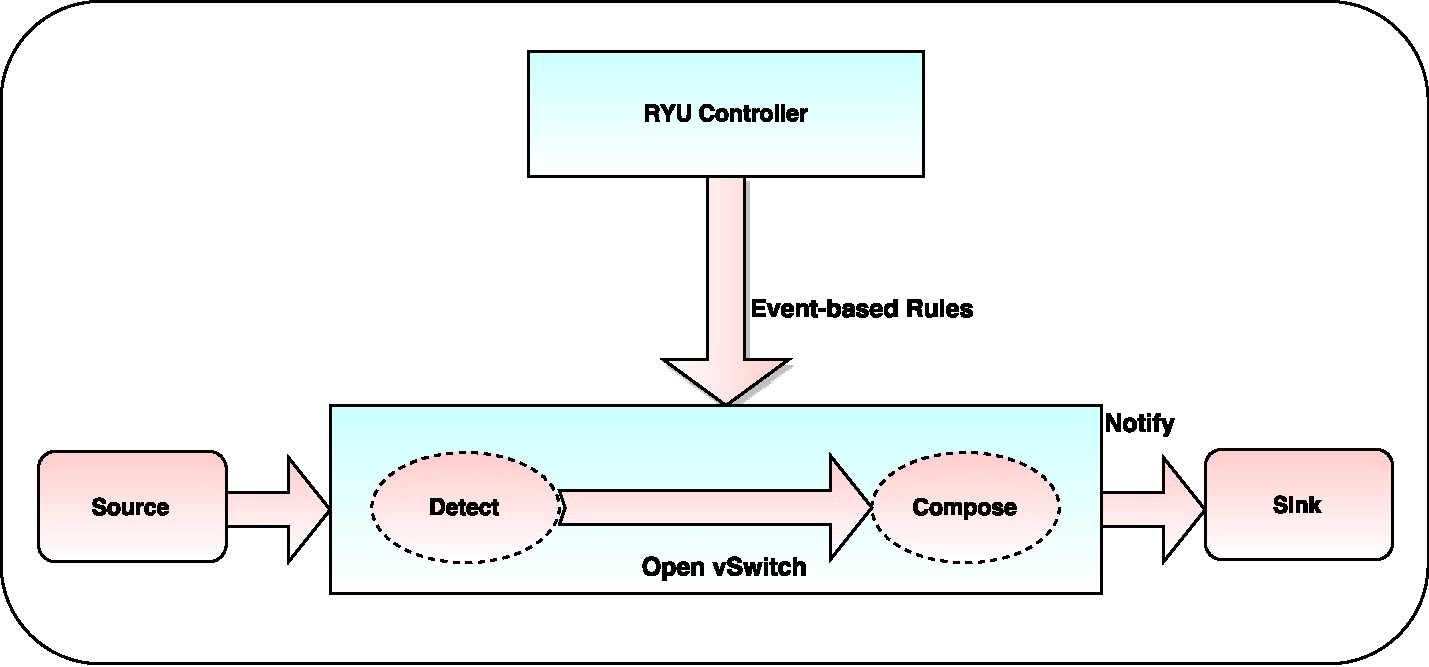
\includegraphics[height=6cm,width=10cm]{evsep01.pdf}
\end{figure}

\section{Goals of the implementation}
Goals of the implementation are defined as below:
\begin{itemize}
\item An Open vSwitch implementation is provided to detect event types and steer them to facilitate staged processing without having to context switch into an intermediate computing node.
\item The Open vSwitch implementation focuses on the DPDK datapath to take advantage of the accelerated packet I/O offered by the DPDK libraries.
\item The Open vSwitch is enabled to execute simple logical operations on the data items of an event and filter based on application logic. 
\item A Ryu controller-based implementation is provided to enable applications to offload user logic on to the vSwitch using an HTTP and JSON based northbound API.
\end{itemize}
Having defined the goals of the thesis, it is important to understand the internals of the Open vSwitch and examine design decisions that need to be taken to achieve the goals outlined.

\section{An overview of Open vSwitch}
In this section a brief overview of the three most important components in the Open vSwitch \cite{pfaff2015design}
\begin{itemize}
 \item \textbf{ovs-vswitchd}: ovs-vswitchd is the generic userspace daemon which speaks OpenFlow and controls all the switches in a system. The ovs-vswitchd daemon is responsible for the OpenFlow pipeline for packet processing and also determines how a packet has to be handled for the first time before it is cached in the datapath. The ovs-vswitchd daemon instructs the datapath on how to handle the packet depending on the configurable OpenFlow processing pipeline. The daemon communicates with the Open vSwitch kernel module via the Netlink interface, and with the ovsdb-server using the custom ovsdb management protocol.
 \item \textbf{ovsdb-server}: The ovsdb-server provides the runtime for the lightweight ovsdb database that holds switch-level configurations. On reboot, the switch configurations are persisted in the ovsdb and are applied when the daemon comes back up. Currently, ovsdb supports state information in the form of 13 different tables for bridges, ports, interfaces, flow tables, controllers, etc. among others.
 \item \textbf{Kernel Datapath}: The kernel datapath or the kernel module is the host operating system implementation of an exact match cache. It is unaware of OpenFlow or the state of the switch. It is kept simple for highly performant packet lookup and forwarding. The ovs-vswitchd receives the first packet from the datapath module, looks up the packet in the OpenFlow processing pipeline, gathers the actions and caches it in the kernel datapath. The following packets of the same flow are forwarded using the caches entries in the datapath without having to go to the userspace daemon(upcall).
\end{itemize}

In addition to the three components is the OpenFlow controller. The controller keeps the state of the network and can be installed on the same server or a remote server. The controller speaks OpenFlow with the ovs-vswitchd daemon and can be used to remotely configure the OpenFlow processing pipeline of several remote switches. The controller may also be used to persist flow of the ovs-vswitchd daemon in the case of a crash. The overview of these components is shown in figure 4.2 - sourced and reinterpreted from \cite{pfaff2015design}.
In addition to the above components, the implementation provides several management utilities:
\begin{itemize}
 \item \textit{ovs-vsctl}: This utility is used to configure the ovsdb-server with several switch configurations such as adding or deleting bridges, adding/deleting ports, etc. The utility connects directly to the ovsdb-server -
 \item \textit{ovs-ofctl}: This utility is used to monitor and configure the OpenFlow switches. It connects directly to the ovs-vswitchd daemon via OpenFlow and provides commands to add new flow rules to the OpenFlow pipelines among several other commands to monitor the flow statistics for the switches and ports.
 \item \textit{ovs-dpctl}: This utility connects to the ovs-vswitchd daemon and provides commands to monitor the cached datapath flows. It offers several commands such as add/delete flows to/from the datapath, monitor statistics, etc. among several others.
 \item \textit{ovs-appctl}: This utility is a used for runtime configuration of the ovs-vswitchd daemon, such as configuring logging levels of the different modules within Open vSwitch.
 \item \textit{ovsdb-tool}: This utility is used to manage the ovsdb files. It offers commands to create DB schemas and compact existing schemas. It does not interact with the ovsdb-server.
 \item \textit{ovsdb-client}: This utility offers a command-line interface to interact with the running ovsdb-server using the different JSON-RPC methods specified by ovsdb management protocol. It offers commands to run transactions such as insert, delete into the ovsdb, dump tables, monitor columns, etc. among others.
\end{itemize}

In the context of the thesis, most of the work focuses on the ovs-vswitchd daemon and the OpenFlow processing pipeline. In the following section the internal flow of data once a packet hits the physical device is presented.

 \begin{figure}[H] 
  \centering   
 \caption{OVS components}
 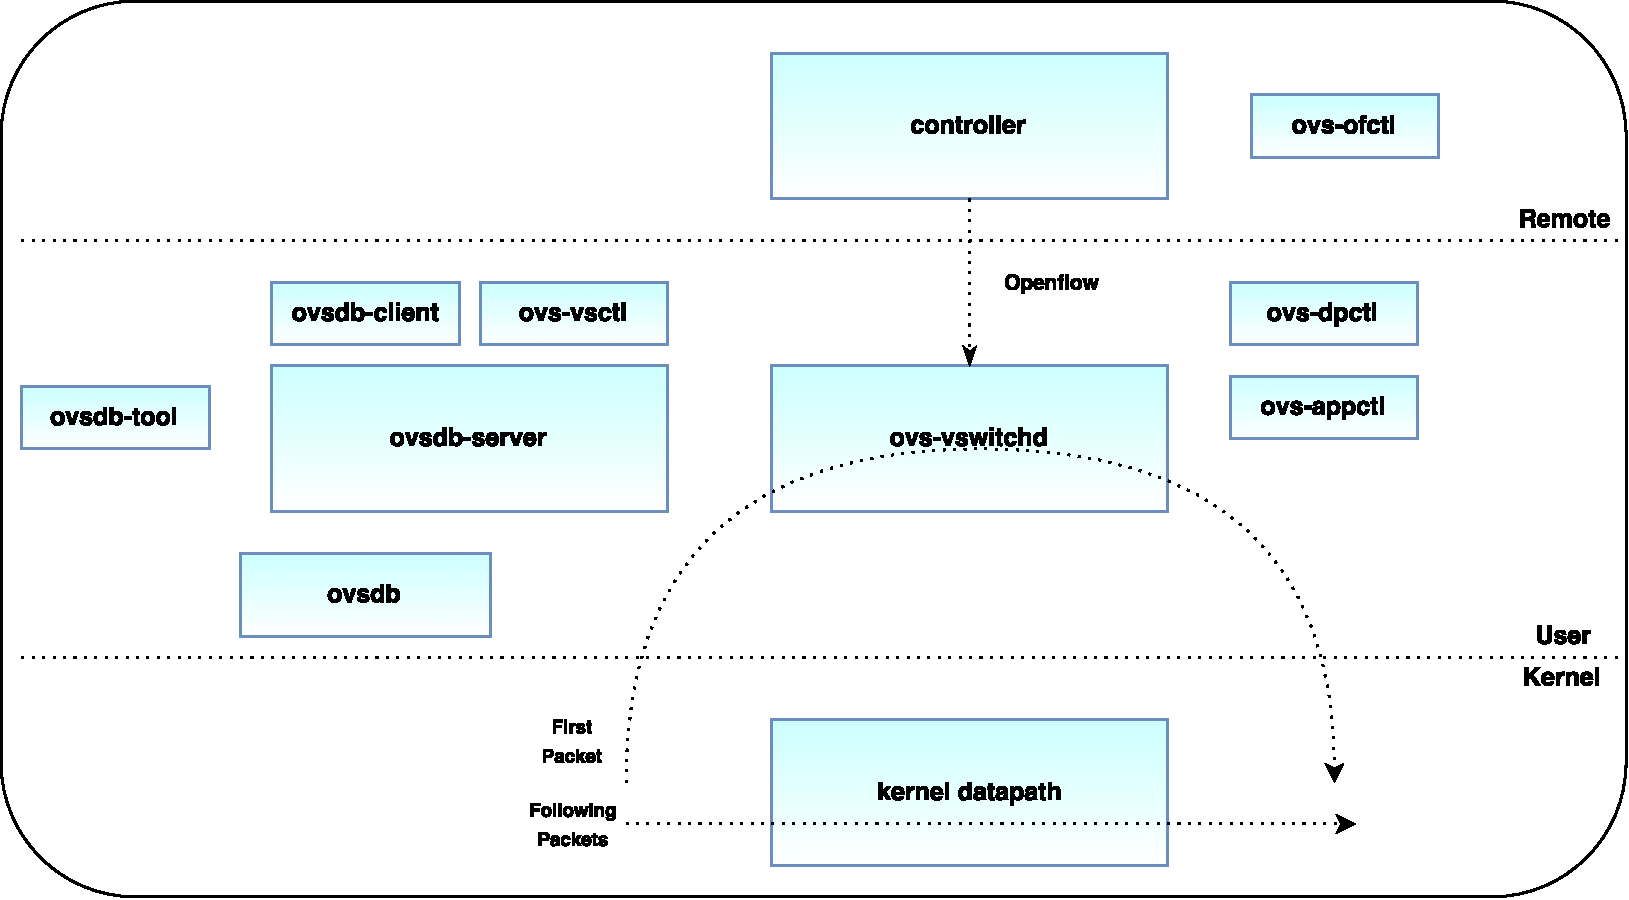
\includegraphics[height=8cm]{kernaldatapath.pdf}
\end{figure}

The interplay of the components of the Open vSwitch is shown in figure 4.3. The two interfaces that specify the handling of the packets are \newline
\textbf{Datapath interface}: The datapath in the context of Open vSwitch is a flow cache capable of forwarding packets through a port. The datapath of an Open vSwitch is implemented specifically to the host machine, and it relies on its clients for intelligence. In this case, the intelligence for the datapath is provided by the ovs-vswitchd. The generic datapath interface provided by Open vSwitch is dpif. The userspace implementation of the datapath interface is provided by the \textit{dpif-netdev} module. The dpif provides an interface with abstractions for three key components:
\begin{itemize}
 \item Ports: Each datapath has a set of ports akin to Ethernet ports. In case of the dpdk or userspace datapaths, the implementation for these ports comes from \textit{struct netdev}, with \textit{netdev-dpdk} specifically handling dpdk ports.
 \item Flow table: A flow table has three key entities: flow - which consists of L2, L3, and L4 headers. The datapath flow uses the \textit{struct dpif-flow}; mask - corresponding to each bit in a flow. The mask field is used for the megaflows, and not for the exact match cache; actions - which tell the datapath what to do with the packet.
 \item Upcalls: The datapath notifies the clients, which is the ovs-vswitchd in this case, about a flow table miss or userspace actions using upcalls. During the upcall, the whole packet is copied to the userspace using the struct \textit{dp_packet}.
\end{itemize}

 \begin{figure}[H] 
 \centering   
 \caption{OVS overview}
 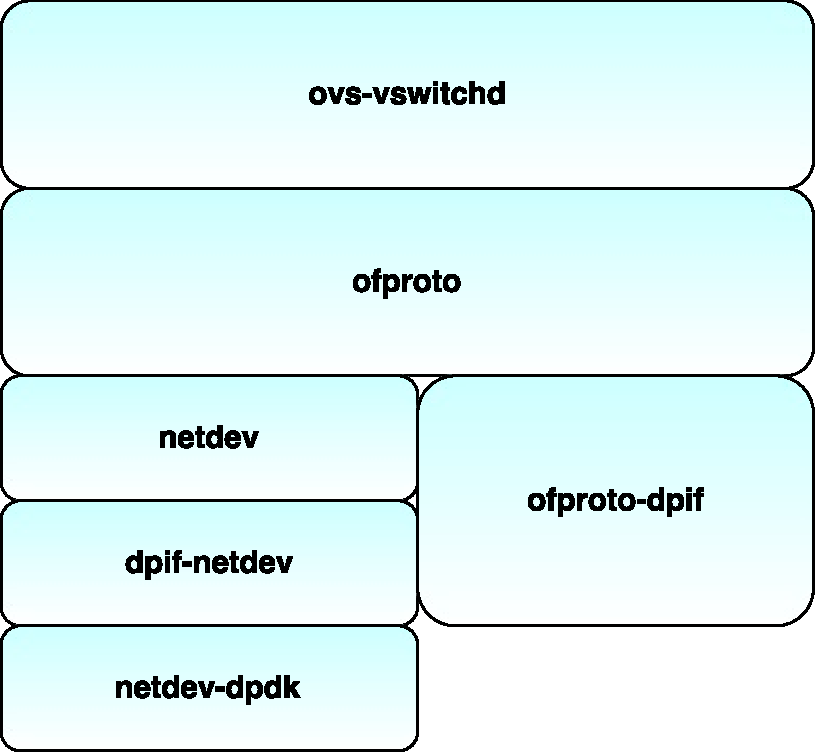
\includegraphics[height=6cm]{internals.pdf}
\end{figure}

\textbf{Ofproto Interface}: The ofproto interface implements the OpenFlow protocol implementation for the dpif-netdev interface. It consists of three major components:
\begin{itemize}
 \item oproto-dpif: This module implements the main provider of the OpenFlow abstraction. It is responsible for installing and removing datapath flows, monitoring and maintaining statistics, etc. The ofproto.dpif module also is responsible for deciding whether a flow is to be cached or not.
 \item ofproto-dpif-upcall: This module performs the role of retrieving the upcalls from the datapath. It performs simple processing of missed upcalls and interacts with ofproto-dpif for complex processing.
 \item ofproto-dpif-xlate: This module performs the role of looking up the OpenFlow processing pipeline, extracting OpenFlow actions and translating into datapath actions.
\end{itemize}

\section{Design Breakdown}
Before design and implementation of the event processing framework within Open vSwitch, a brief breakdown of the design and rationale is provided. The design details are presented in the later sections. Key aspects that require our focus are:
\begin{itemize}
 \item Extraction of events from the payload: While work done by  Mekky et. al \cite{mekky2014application} concentrates on creating OpenFlow actions to direct packets into a separate application module to work on the payload, the work in this thesis focuses on extracting the payload at line rate. The rationale behind this approach is that event queries are applied on each packet in the system, and directing the packets to a separate application module is expensive when the same action has to be repeated for every single packet.
 \item De-serializing the event payload: The data items in the event stream are encoded. In the thesis, a solution is provided for de-serializing hexadecimal encoded streams of data. 
 \item Accessing the event data: Once the event items are extracted and encoded from the event stream, they must be made accessible for processing within the Open vSwitch and also be accessible by OpenFlow rules that are installed on the controller. Due to this reason, the design focuses on modifying the OpenFlow 1.0 protocol spoken between the controller and the Open vSwitch. Although OpenFlow 1.3 is the most standard protocol in use, the work in the thesis uses OpenFlow 1.0 for simplicity. Porting from OpenFlow 1.0 to 1.3 is not considered to be a blocking factor.
 \begin{figure}[H] 
 \centering   
 \caption{OVS dataflow: datapath to ofproto}
 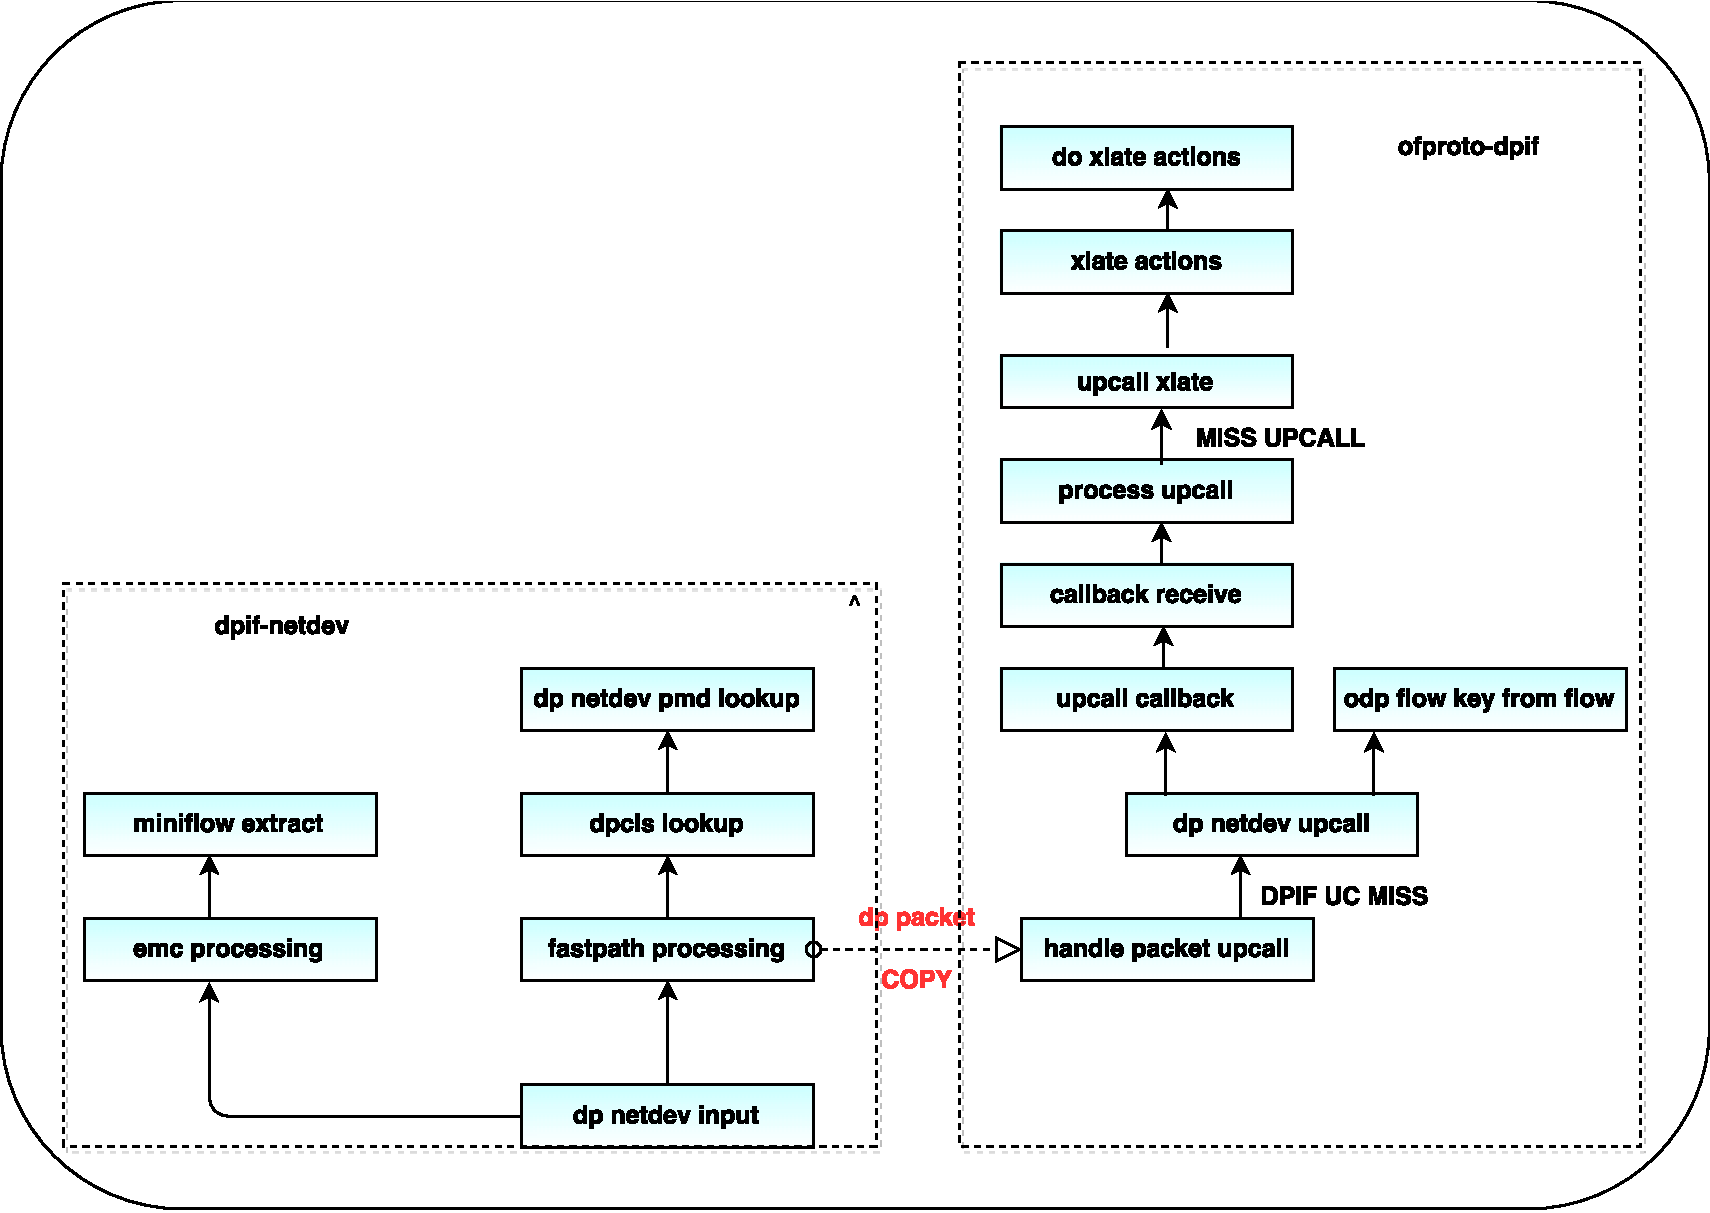
\includegraphics[height=8cm]{dpnetdev.pdf}
\end{figure}
 \item OpenFlow pipeline support for events: For making the event detection programmable, additional tables are created within the OpenFlow processing pipeline, or the ofproto classifier. Handling the ofproto classifier is sufficient because ofproto-dpif takes care of creating the tables in the datapath classifier/exact match cache when needed.
 \item Creating keys for event attributes: The \textit{odp-netlink} interface in Open vSwitch specifies the rules for creating attribute keys. These keys are used to look up the ofproto classifier and find the relevant rule installed for an event. 
 \item Support for logical operations: The operations on event attributes are performed using OpenFlow actions. Hence each operation is achieved using a newly defined action, which is triggered based on the detection criteria specified on event items.
 \item RYU Controller design: The controller plays a big role in communicating OpenFlow rules to the Open vSwitch. Although ovs-ofctl utility can also play this part, a controller such as RYU is more sophisticated, in that it allows the creation of HTTP API's that are accessible by remote webservers to create rules. Such an API support is provided which enables remote creation and deletion of event based rules. From the event processing perspective, the RYU controller plays the role of the rules engine, whereas Open vSwitch plays the role of the execution engine. 
\end{itemize}

The design overview presented above aims to create a sophisticated programmable event processing framework on the network, which can complement the event processing engines to achieve latency sensitive results, reduce the burden on the network and enable staged processing. In the coming sections, more focus is granted up on individual design decisions.


\section{System Model}
In this sections, the supported semantics for event processing within the Open vSwitch is presented. Each event follows the below representation:\\1. Unique Tag\\
2. Event Type\\3. Event Attributes


To this end the event payload format processed by the framework within Open vSwitch is pre-defined. Each event has a unique tag,  followed by the event type and two event attributes. Only the packets with the unique tag are processed through the event processing pipeline. In other cases, the packets are taken through the standard processing pipeline within Open vSwitch. The event payload handled by the event processing engine is shown in figure 4.5. The timestamp in the event is used for evaluation purposes.

\begin{figure}[H]
 \centering
 \caption{Event Payload}
 \includegraphics[width=10cm]{payload.pdf}
\end{figure}

\subsection{Event Detection Semantics}
Let 'E' be an event of type 't' and attributes '$a_1$' and '$a_2$'.

\begin{equation}
E\lbrace t,a_1,a_2 \rbrace
\end{equation}

The event detection semantic understood and processed by the framework are described below:

\begin{flushleft}
 Event instances can be detected based on different variants.
 \\1. Detect based on Event Type
 \\2. Detect based on values in Event Attributes
 \\3. Detect based on combination of Event Type
 \\
\end{flushleft}
\begin{flushleft}
 Event detection operations can be combined with logical operators:
 \\
 \textbf{Conjunction}: Event is signalled when all constituent input patterns evaluate to True. 
 \\
 \textbf{Disjunction}: Event is signalled when atleast one constituent input pattern evaluates to True.
 \\

\end{flushleft}


\begin{flushleft}
The detect operations that are implemented are denoted as:

\begin{equation}
D(e.t) \quad | \quad stream
\end{equation}
\begin{equation}
D(e.t) \quad | \quad filter
\end{equation}
\begin{equation}
D(e.t  \wedge e.a_1) \quad | \quad stream
\end{equation}
\begin{equation}
D(e.t  \wedge e.a_1) \quad | \quad filter
\end{equation}
\begin{equation}
D(e.t  \wedge e.a_2) \quad | \quad stream
\end{equation}
\begin{equation}
D(e.t  \wedge e.a_2) \quad | \quad filter
\end{equation}
\begin{equation}
D(e.t  \wedge (e.a_1 \wedge e.a_2)) \quad | \quad stream
\end{equation}
\begin{equation}
D(e.t  \wedge (e.a_1 \wedge e.a_2)) \quad | \quad filter
\end{equation}
\begin{equation} 
D(e.t  \wedge (e.a_1  \vee e.a_2 )) \quad | \quad stream
\end{equation}
\begin{equation} 
D(e.t  \wedge (e.a_1  \vee e.a_2 )) \quad | \quad filter
\end{equation}

where \textit{D} is the detect operation; \newline
| denotes the redirect operation; \newline
\textit{stream} is the logical stream to which the detected event is redirected to.\newline
\textit{filter} is the operation to filter the detected event \newline \newline
\end{flushleft}


\subsection{Compare Operation Semantics}
In addition to event detection based on match of event attributes, compare operations on event attributes are implemented. The set of implemented compare operators is given by:
\begin{equation}
\oplus  \ni  \lbrace <=,>= \rbrace
\end{equation}

and the possible operations using the compare operators is given by:
\begin{equation}
D(e.t  \wedge (e.a_1 \oplus value) \vee e.a_2) \quad | \quad filter
\end{equation}
\begin{equation}
D(e.t  \wedge (e.a_1 \oplus e.a_2) \quad | \quad filter
\end{equation}
\subsection{Stateful Operation Semantics}
Stateful operations in the context of the implementation are defined as those that use the knowledge of previous events to take an action on the currently detected event. The two stateful operations implemented are moving maxima and window.

\begin{equation}
D(e.t  \wedge (e.a_1  <=\quad \rightarrow maxvalue) ) \quad | \quad filter
\end{equation}
In this operation all the events with attribute lower than the given \textit{maxvalue} are filtered. However, on the detection of an event with a value higher than the given \textit{maxvalue}, the event is forwarded and the newly seen value becomes \textit{maxvalue}.
\begin{equation}
D(e.t  \wedge (e.a_1  <=\quad \overrightarrow{win} \quad maxvalue)) \quad | \quad filter
\end{equation}
Similar to 4.15,  all the events with attribute lower than the given \textit{maxvalue} are filtered. However, on the detection of an event with a value higher than the given \textit{maxvalue}, the event is forwarded and the newly seen value becomes \textit{maxvalue}. The \textit{maxval} increases for a window of \textit{win} events after which it remains steady. if the window is 0, this is equivalent to less than or equal to operation defined in 4.14.

\section{Implementation walk-through}
In this section, the key aspects of implementing a programmable event processing framework within an Open vSwitch are discussed. The implementation aims to meet the specifications defined in the system model in section 4.5 and follows the design strategy discussed in section 4.4. Wherever appropriate the implementation is discussed along with data or control flow diagrams, snippets of code or data structures used in the implementation.

\subsection{Event extraction and de-serialization}
In this section, the methodology for event parsing and extraction is presented. Before chalking up a strategy, the flow of data in the DPDK/userspace datapath is examined more closely in figure 4.4. As it can be seen in the figure, the packet is handed over to the ofproto interface in its entirety using the data structure \textit{dp_packet}. But if the event data is extracted only after passing it to ofproto, this would mean that any support of the exact match cache or the datapath classifier that can be provided by the DPDK datapath to the event processing extension is ruled out. Hence the parsing and extraction of the event payload is done within the dpif-netdev implementation using the flow module. Once the event is extracted, it is de-serialized. Both the steps are done within the flow module of the Open vSwitch. 

\begin{figure}[H]
 \centering
 \caption{Event extraction and deserialization}
 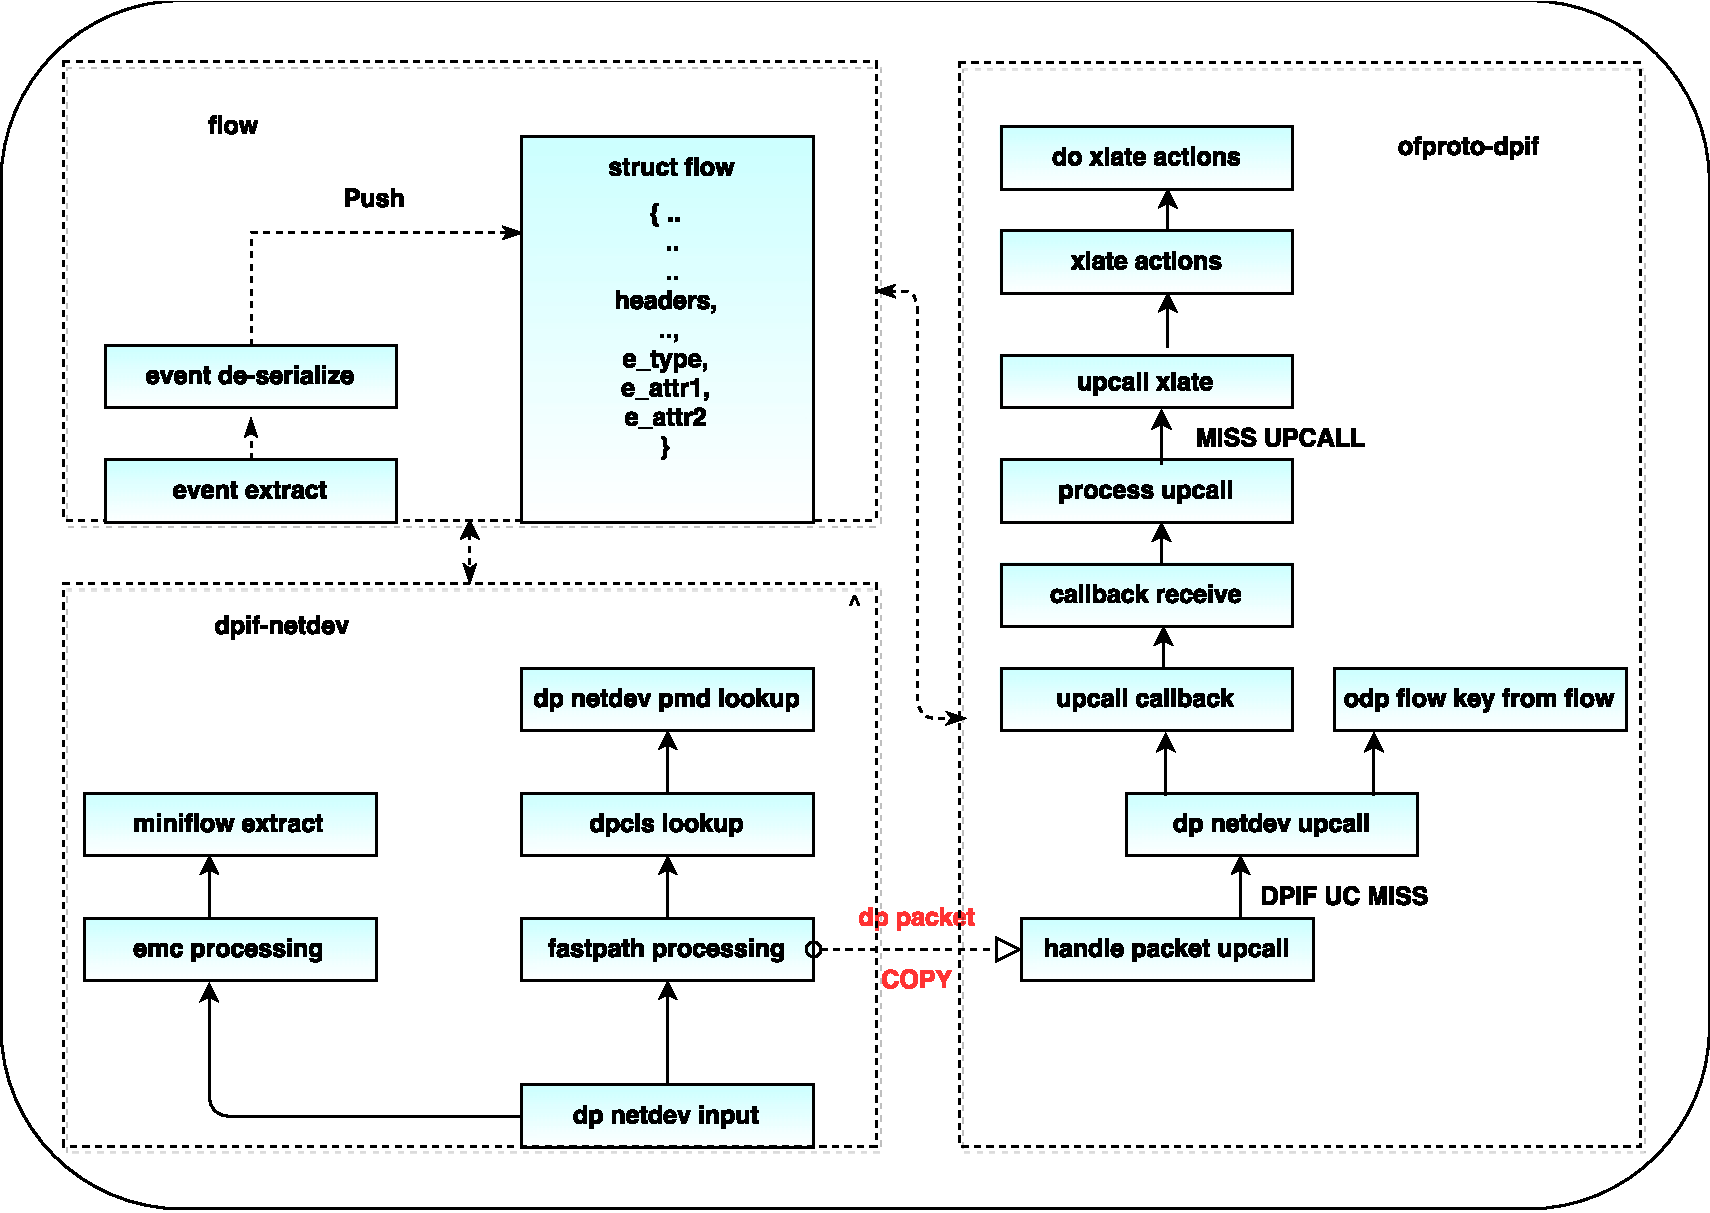
\includegraphics[height=8cm]{flowextract01.pdf}
\end{figure}

\subsection{Accessing event data}
Once the data items are extracted and de-serialized, they are being made accessible to the implementations of both the ofproto interface and datapath interface. The flow module of the Open vSwitch specifies the data structures for the OpenFlow fields, which are accessible by both the userspace dpif-netdev and ofproto implementation. Additionally, since the extraction and de-serialization of the event data is performed within the flow module, the support for event data items is added into the userspace flow data structure \textit{struct flow}. Doing so ensures that the event data is accessible to the ofproto and the datapath interface, and also to the yet to be discussed meta-flow module which specifies the interface for the Open vSwitch implementation of OpenFlow 1.0 tables. Figure 4.6 shows the interplay of the modules while extracting, de-serializing and pushing the data to the relevant data structure for access within other modules. The flow module also provides another data structure \textit{struct flow_wildcards} which follows the same structure as flow, except that each 1-bit in wildcard indicates that the corresponding bit in \textit{struct flow} must match. For the event data items, only an exact match is supported. Hence all the bits of the struct \textit{flow_wildcards} for event data items are set. Below snippet shows the addition of support for event data in struct flow and the map used to access the flow by other interfaces. \newline

\begin{lstlisting}[language=c]
struct flow {
..
..
..
/* L4 (64-bit aligned) */
ovs_be64 e_type;
ovs_be64 e_attr1;
ovs_be64 e_attr2;
..
..
}

FLOWMAP_SET(map, e_type);  
FLOWMAP_SET(map, e_attr1);  
FLOWMAP_SET(map, e_attr2);  


miniflow_push_be64(mf, e_type, htonll(event[0]));                   
miniflow_push_be64(mf, e_attr1, htonll(event[1]));
miniflow_push_be64(mf, e_attr2, htonll(event[2]));
\end{lstlisting}



\begin{figure}[H]
 \centering
 \caption{Openflow Pipeline}
 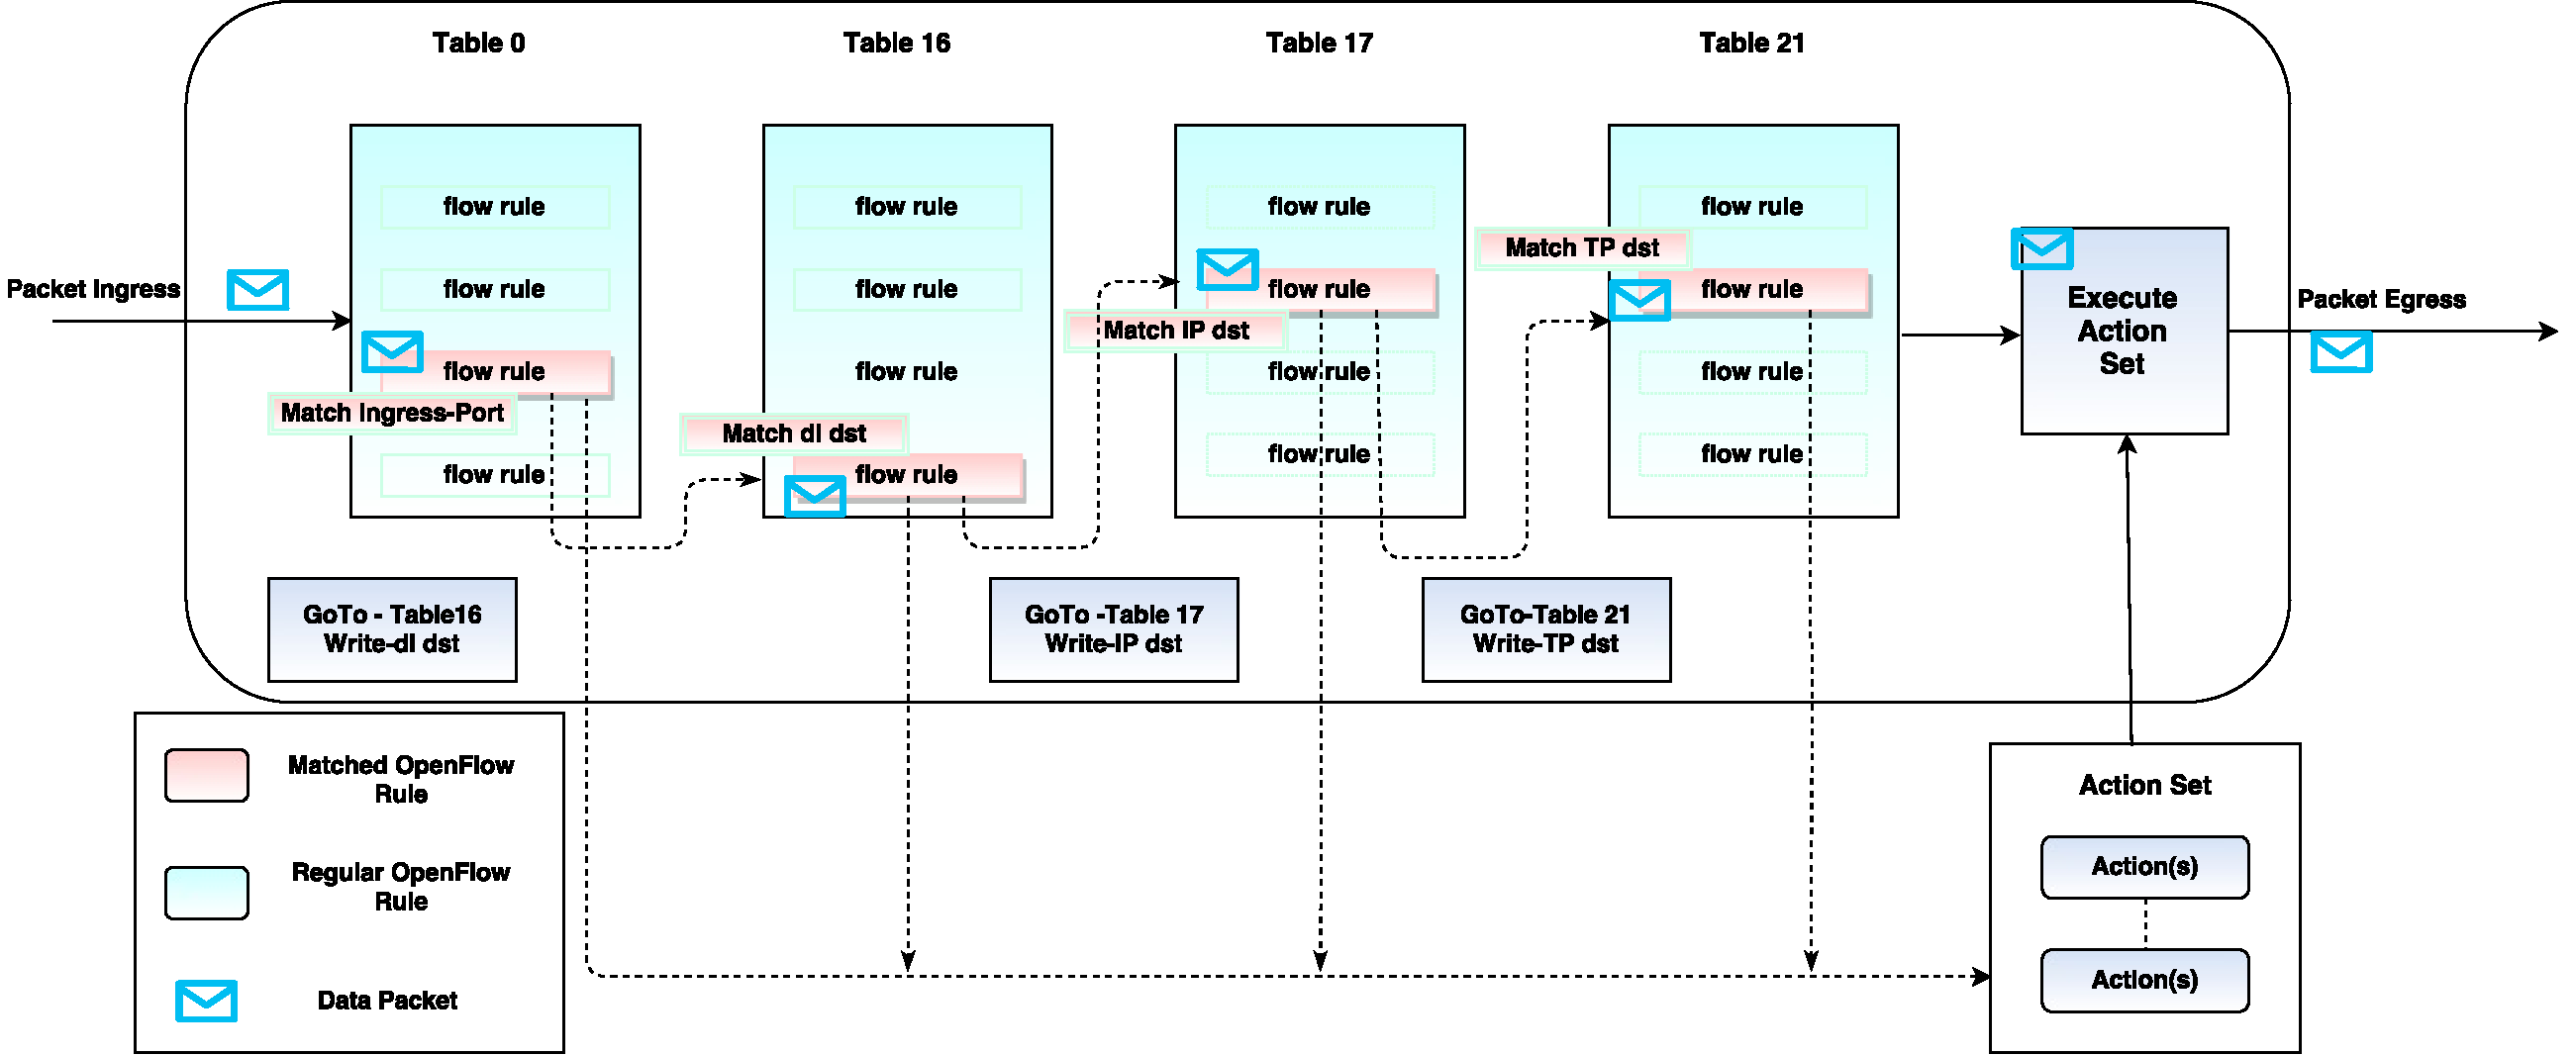
\includegraphics[height=8cm,width=19cm]{pipeline05.pdf}
\end{figure}

\subsection{Modelling OpenFlow pipeline for event processing}
As briefly alluded to in the section 4.6.2, the event items are to be added into the OpenFlow processing pipeline. The specification of OpenFlow 1.0 protocol is available within Open vSwitch in the Openflow-1.0 modules. The meta-flow module defines the interface to implement the OpenFlow processing pipeline, i.e., the fields of the ofproto classifier. Before diving into the implementation details, we examine the ofproto classifier pipeline in figure 4.7. OpenFlow supports pipelined processing of packets with the help of multiple tables which in turn have multiple flow rule entries. In figure 4.7, the incoming packet at the ingress port is matched at Table 0, the action of rewriting the mac destination address is added to the action-set and submitted to Table 16. At Table 16, the packet is matched on its mac destination address, and the action of re-writing its IP destination address is added to action-set is performed, and it is forwarded to Table 17. At Table 17, the packet is matched by a flow rule for its IP destination address, and the action of re-writing its Transport destination address is added to the action-set, and the packet is forwarded to Table 21. At Table 21 the packet is matched by a flow rule for its Transport destination address and checked for GO-TO instruction in rule action. Since no GO-TO instruction is found, the pipeline processing stops and the action-set is executed on the packet, and the packet is forwarded through the egress port. For the sake of simplicity, the focus in this thesis document will be on a single OpenFlow table. Although enabling one OpenFlow table to handle event data is sufficient to create an OpenFlow pipeline for event data, such a use case is not helpful initially. Figure 4.8 shows an individual flow table and the steps taken to enable event fields within it. 

\begin{figure}[H]
 \centering
 \caption{Openflow Flowtable - Add event data fields}
 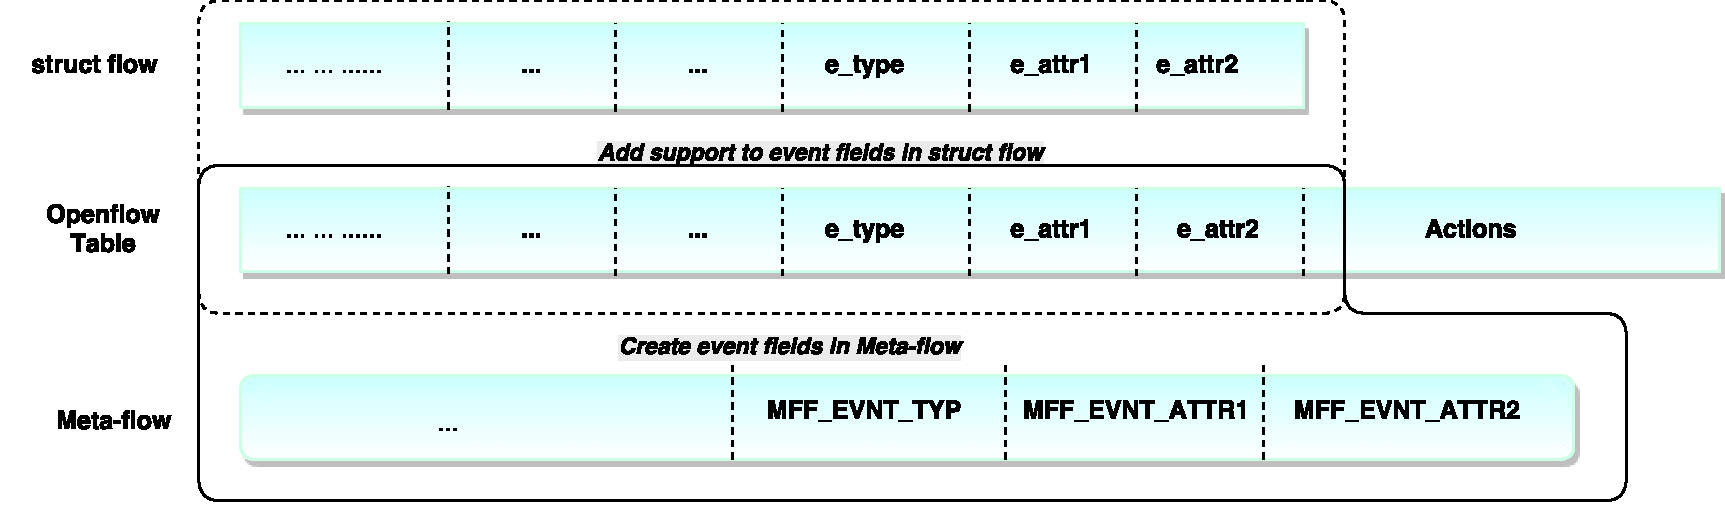
\includegraphics[height=4cm]{flowtable.pdf}
\end{figure}

\subsection{Adding event data fields to OpenFlow tables}
 As discussed in section 4.6.2 the data structure flow is modified to handle event data and provide access to the event data to the ofproto interface. Predictably, similar support is to be added to the OpenFlow table using the meta-flow module as shown in figure 4.8. Below is the snippet which shows the creation of the event type as an OpenFlow field within the meta-flow module. \newline

\begin{lstlisting}
/* "e_type".
*
* Event Type.
*
* Type: be64.
* Maskable: bitwise.
* Formatting: decimal.
* Prerequisites: UDP.
* Access: read/write.
* NXM: NXM_OF_EVNT_TYP(113) since v2.6.
* OXM: OXM_OF_EVNT_TYP(46) since OF1.2 and v2.6.
* OF1.0: exact match.
* OF1.1: exact match.
*/    
MFF_EVNT_TYP,
\end{lstlisting}


The comments for the meta-flow field are expected to be in the exact format specified for the python helper function extract-ofp-fields. Failing to do so results in build breakdown. In addition to adding fields in the meta-flow module, the fields are provided with necessary helper functions which are accessed by ofproto and ofp-parse interfaces while responding to flow-mod or flow stats request commands from the controller. One such helper function defined to set e_type from the corresponding met-flow field is shown below. This function is used to read the meta-flow field and populate match before dumping the buffer for dump-flow commands. Similarly, other helpers are defined. \newline
\begin{lstlisting}[language=c]
void
mf_set_value(const struct mf_field *mf,
const union mf_value *value, struct match *match, char **err_str)`{
 ..
 ..
 case MFF_EVNT_TYP:
 match_set_event_type(match, value->be64,OVS_BE64_MAX);
 break; 
 ..
 ..
 
}
\end{lstlisting}

\subsection{Adding support for event based rules}
Adding event fields in the meta-flow module enables support for event data in the OpenFlow table. It, however, is not sufficient to enable event-based rules and detection of events based on extracted data. This is done in two stages
\begin{itemize}
\item Provide support to event fields in add-flow command of ovs-ofctl utility to send the relevant data in OpenFlow message. This command is also used by the controller. More about the controller implementation is discussed later.
\item Add support to decode event fields from the incoming OpenFlow message and insert the event based rules into the classifier.
\end{itemize}
Before diving into the details, the important interfaces are examined:
\begin{itemize}
\item \textbf{ofp-parse interface}: The ofp-parse interface specifies the layer of communication between ovs-vswitchd and OpenFlow. In the case of the flow-mod commands(OFPC_ADD), ofp-parse module converts the string value pairs of the event fields and inserts them into the match field of data structure \textit{struct ofp_util_flow_mod}.
\item \textbf{ofp-util interface}: The ofp-util interface defines the the \textit{struct ofp_util_flow_mod} to consume and respond to the flow-mod commands. The struct \textit{struct ofp_util_flow_mod} is composed of a struct match as a member. 
\item \textbf{match interface} The match interface provides the data structure for flow classification - \textit{struct match}. Each match structure consists of a flow and a corresponding wildcard.  The ofp-parse and ofp-util interface combine to extract the string-value pairs in a flow-mod command into relevant flows and wildcards within a \textit{struct match}. 
In addition to creating event based flow rules, functionality is also implemented to dump event based flow rules on to the buffer as in case of dump-flows command. For this operation, within the match module, helper functions to get meta-flow event fields into the \textit{struct match} are also defined. This is used by the ofp-parse interface to populate \textit{struct match} and hand it over to nx-match interface for encoding. An example of such an helper function is shown in the below snippet: \newline
\begin{lstlisting}[language=c]
void
match_set_event_type_masked(struct match *match, ovs_be64 e_type, ovs_be64 mask){
match->flow.e_type = e_type & mask;
match->wc.masks.e_type = mask;
}
\end{lstlisting}

\item \textbf{nx-match module}: The flow and the wildcards from the match interface are encoded as fields defined by the meta-flow module using the nicira extension helper functions specified by the nx-match module. Doing so enables dump-flow support to event-based rules.
\end{itemize}

Figure 4.9 shows how a OFPFC_ADD command with event fields is parsed and normalized into the match interface using \textit{struct ofputil_flow_mod}. To enable correct parsing of the event fields, OpenFlow 1.0 support is configured in Openflow-1.0 header file: \newline

\begin{lstlisting}[language=c]
enum ofp10_flow_wildcards {
..
OFPFW10_EVNT_ATTR1 = 1 << 22,
OFPFW10_EVNT_ATTR2 = 1 << 23,
OFPFW10_EVNT_TYP   = 1 << 24,
..
}
\end{lstlisting}
This informs the parser that the relevant event fields are in the 22, 23 and 24 positions of the character string. After which the relevant event fields are populated and normalized. Normalization ensures that the corresponding wildcards for the match flow entries are appropriately set. Once normalized the flow-mod command is encoded as a OFPT_FLOW_MOD message and send to the ovs-vswitchd daemon which actively polls for OpenFlow messages.

\begin{figure}[H]
 \centering
 \caption{Openflow: Parse event fields}
 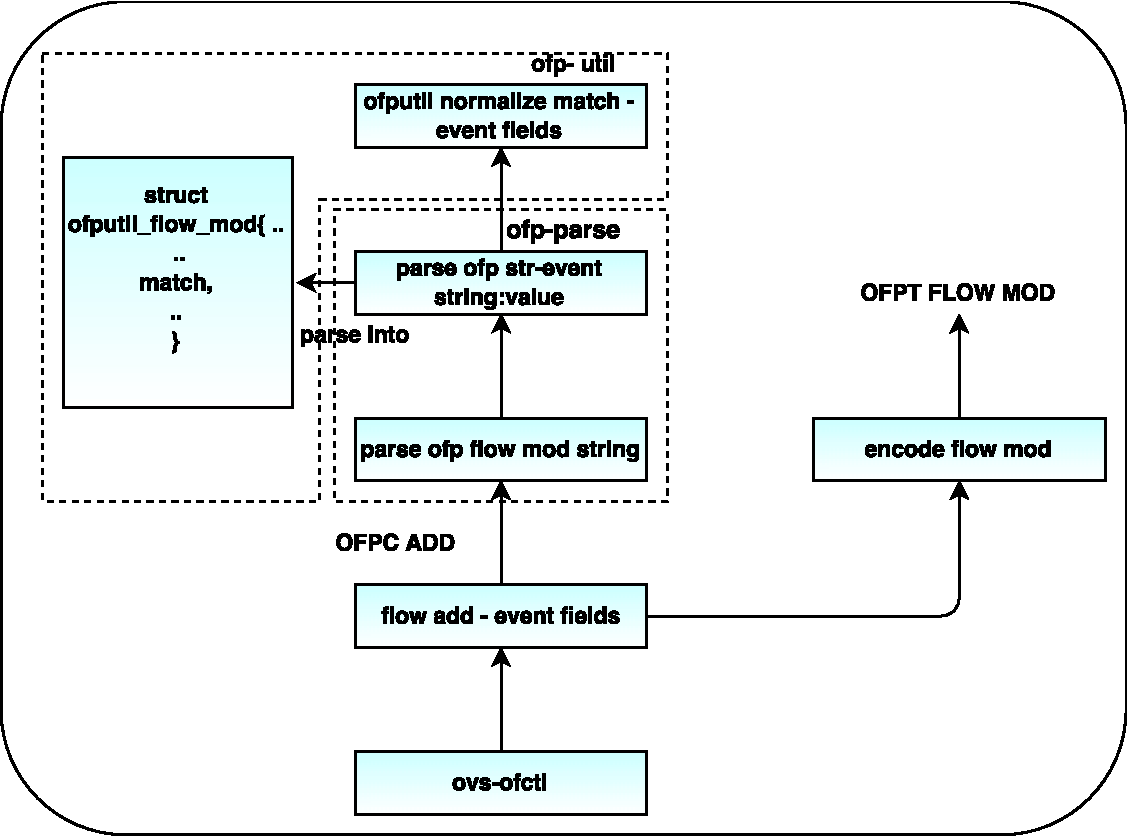
\includegraphics[height=9cm]{flowadd01.pdf}
\end{figure}

Figure 4.10 shows an OpenFlow message of type OFPTYPE_FLOW_MOD is parsed to extract the relevant rules and added into the classifier. The ovs-vswitchd daemon actively polls for OpenFlow messages. On receiving a message, the message type is decoded. If the message is of type 'OFPTYPE_FLOW_MOD' the message is decoded by a decode function. The first phase of the decoding process involved pulling the message which is in the custom OpenFlow buffer, ofpbuf, into the Openflow1.0 match structure struct ofp10_match. This structure is also extended to support event fields, very much like struct flow: \newline

\begin{lstlisting}[language=c]
struct ofp10_match {
..
ovs_be64 e_attr1;
ovs_be64 e_attr2;
ovs_be64 e_type;
}
\end{lstlisting}

Once the \textit{struct op10_match} is created, the relevant event fields are extracted and put into a \textit{struct match} and normalized. The ofpbuf is not directly pulled into \textit{struct match} because the match interface is inaccessible outside the context of ovs-vswitchd. Instead, the ofp-util interface is used to convert the data OpenFlow structures to a form understandable and accessible by the OpenFlow implementation within Open vSwitch, i.e., ofproto. Once the rules are stored in the form of a match, the ovs-vswitchd daemon calls the ofproto interface to add the rules into the classifier.

\begin{figure}[H]
 \centering
 \caption{Openflow: Event rule creation}
 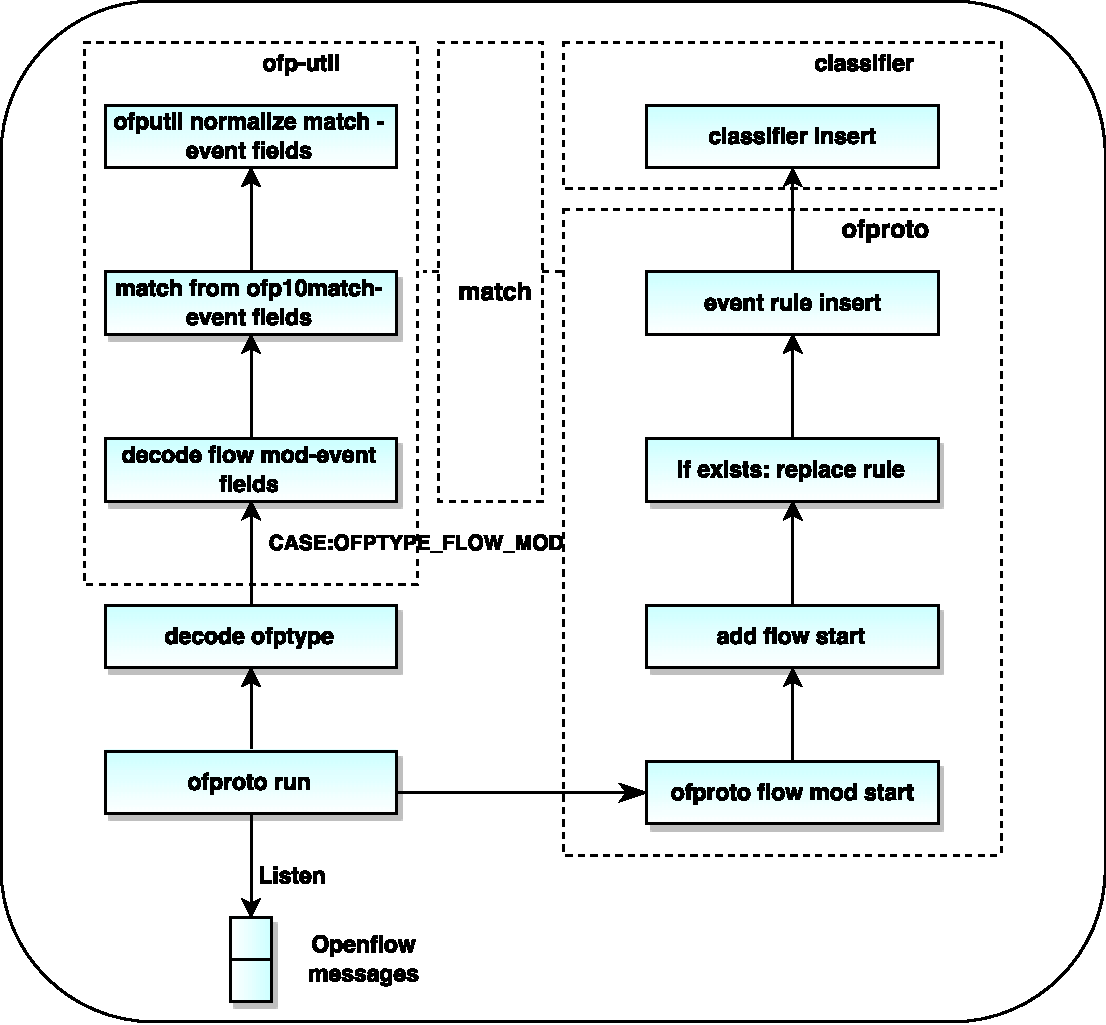
\includegraphics[height=9cm,width=11cm]{ruleinsert01.pdf}
\end{figure}

At this point, the implementation supports programmable event rules and the three event fields specified by the system model. However, the event detection mechanism is yet to be implemented. In the next subsection, a closer look into the implementation steps needed to support matching based on event type and event attributes is presented.

\subsection{Detection based on event data}
In this section, the implementation process to support classifier lookup based on event fields. In section 4.6.2, event data is pushed into the flow structure, and in section 4.6.3 to 4.6.5, event rule support is added to the OpenFlow processing tables- i.e., ofproto classifier. To look up the classifier with the event data items, event keys are extracted from the flow. Figure 4.11 illustrates the lookup process followed by the ofproto-dpif-xlate module.

\begin{figure}[H]
 \centering
 \caption{ofproto: Rule look-up}
 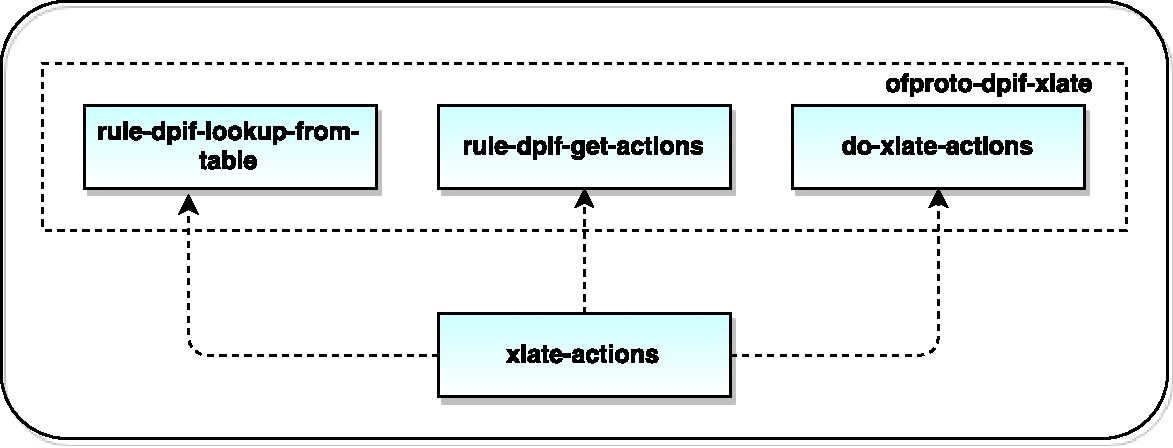
\includegraphics[height=4cm]{ofproto-dpif-xlate.pdf}
\end{figure}

Userspace keys to support the lookup are added to odp-netlink. In the below snippets, the set up steps for \textit{e_type} key are shown. The snippet focuses on the key steps to be taken to enable keys and excludes the details, which can be found in the source code. \newline

\begin{lstlisting}[language=c]
enum ovs_key_attr {
..
#ifndef __KERNEL__
/* Only used within userspace datapath*/ 

OVS_KEY_ATTR_EVNT_TYP,
#endif
..
};

struct ovs_key_etype {
ovs_be64 e_type;
};

\end{lstlisting}

and the keys are parsed and extracted to be used by ofproto-dpif. \newline
\begin{lstlisting}[language=c]
/* parse_l2_5_onward */
if (!is_mask) {
..
..
 expected_attrs |= UINT64_C(1) << OVS_KEY_ATTR_EVNT_TYP;
}

if (present_attrs & (UINT64_C(1) << OVS_KEY_ATTR_EVNT_TYP)) {
 const struct ovs_key_etype *etype_key; 
 etype_key = nl_attr_get(attrs[OVS_KEY_ATTR_EVNT_TYP]);
 put_etype_key(etype_key, flow);
}

/* odp_flow_key_from_flow  and odp_flow_key_from_mask*/
 struct ovs_key_etype *etype_key;  
etype_key = nl_msg_put_unspec_uninit(buf, OVS_KEY_ATTR_EVNT_TYP,
sizeof *etype_key); 
\end{lstlisting}

At this stage, the implementation supports event rules that implement operations denoted through 4.2 to 4.11, by combining existing event semantics with drop and mod actions provided by OpenFlow. In Section 5.4.7, many of these operations are evaluated with their respective rule format supported by the RYU controller. The operations are also contrasted with their expression in a standard Event Query language.



\subsection{Enabling compare operations support}
As discussed in section 4.2, the thesis also aims to provide support for logical operations on event attributes. In section 4.5.2 the two compare operators {>=, <=} are outlined for implementation. In this section the implementation of the compare operations within Open vSwitch is presented. The operations are implemented as Openflow actions which are triggered after detecting a event type. The two compare operations are implemented as:
\begin{itemize}
 \item \textbf{set_max} : A \textit{set_max:val} action ensures that any event with attribute value higher than \textit{val} is filtered out for a particular event type.
 \item \textbf{set_min} : A \textit{set_min:val} action ensures that any event with attribute value lower than \textit{val} is filtered out for a particular event type.
\end{itemize}
The \textit{set_max}, \textit{set_min} actions provide implementation support for operations denoted in 4.13. The implentation can be extended for any binary operaiton The code snippets illustrate  how the new actions are added to the Openflow action list, with \textit{set_max} action used for illustration. \newline

\begin{lstlisting}[language=c]

OFPACT(SET_MAX,ofpact_attr, ofpact, "set_max")      
/* OFPACT_SET_MAX.
*
* Used for OFPAT10_SET_MAX.*/
struct ofpact_attr {
 struct ofpact ofpact;
 uint64_t attr;              /* Attribute value. */
};
\end{lstlisting}

In addition implementation support is provided to parse, decode, encode and set attributes for actions. The implemetnation for the user actions is done in the ofproto-dpif-xlate module which as discussed before and illustrated in figure 4.11 is responsible for deriving actions and performing them. \newline
\begin{lstlisting}[language=c]
case OFPACT_SET_MAX:{        
 if(htonll(flow->e_attr1) <= ofpact_get_SET_MAX(a)->attr){
  xlate_normal(ctx);
 }
 break;    
}
\end{lstlisting}

In addition to comparing attributes to values provided in event rules; another class of action is implemented which allow creation of rules to compare between the attributes themselves. This is done via:
\begin{itemize}
 \item \textbf{attr_cmp}: A \textit{attr_cmp:mode} action compares the event attributes, and filters out the events based on the mode triggered by \textit{val}. if \textit{mode} is 0, only events with equal attributes is forwarded, rest are dropped. if \textit{mode} is 1, only events with attribute 1 greater than attribute 2 are forwarded, if \textit{mode} is 2, only events with attribute 2 greater than attribute 1 are forwarded. Here \textit{mode} triggers the operation to be used between attributes. Similarly implementations can be extended for any other binary operation.
\end{itemize}
The  \textit{attr_cmp} action provides the implementation of operations denoted in 4.14.

\subsection{Enabling Stateful Operations}
In this section the implementation of stateful operations denoted in section 4.5.3 is detailed. To implement these operations two actions are implemented:
\begin{itemize}
 \item \textbf{mov_max}: A \textit{mov_max:maxval} action filters the event if the attribute is lower than \textit{maxval}. However if the attribute value higher than \textit{val} is encountered, the event is forwarded and the newly seen value becomes the new \textit{maxval}. This action provides implementation support to the operation denoted in 4.15. Below the pseudo-code of the \textit{mov_max} action is shown:\newline
 \begin{lstlisting}[language=c]
 case OFPACT_SET_MOV_MAX: 
 mov_max= ofpact_get_SET_MOV_MAX(a)->attr
 item= search_max(type)
 if(item!=NULL):                         
  cur_max = item->data
  if(attr1 > cur_max):
   delete_max(item)
   insert_max(type, attr1)                
 else:
  cur_max = mov_max
  insert_max(type, mov_max)
 if(attr1 < cur_max):
   break
 else:  
  xlate_normal(ctx)  
  break  
 \end{lstlisting}
 
 \item \textbf{set_win,win_max}: The combination of \textit{set_win:win,win_max:maxval} actions performs a similar role done by the \textit{mov_max}. However the \textit{maxval} is incremented only for the specified window \textit{win}, after which it remains constant. To understand this action, let us look at an example for event type 'TEMP', with action \textit{set_win:10,win_max:50}. Firstly all events of type 'TEMP' with attribute values lower than 50 are filtered. An event of type 'TEMP' and attribute value 60 is forwarded, and 60 becomes the new \textit{maxval}. And going forward, a 'TEMP' event with value 58 will be filtered. This increment of \textit{maxval} continues till the 10th window, or otherwise the 10th time the rule is hit. From thereon, the highest value of attribute seen within the defined window will remain the \textit{maxval}. This action provides implementation support to the operation denoted in 4.16. The below pseudo-code glimpses through the implementation.
 
\begin{lstlisting}[language=c]
case OFPACT_SET_WIN:
window= ofpact_get_SET_WIN(a)->attr
winItem=search_window(type)
if(winItem == NULL):
 insert_window(type, window, 0)                       
else:
 delete_window(winItem)
 insert_window(type, window, ++(winItem->counter))       
break;

case OFPACT_SET_WIN_MAX:
mov_max= ofpact_get_SET_WIN_MAX(a)->attr 
winItem=search_window(type)
item= search_max(type)
if(>window <= counter):
 if(item!=NULL):
  cur_max = item->data 
 else
  cur_max = mov_max
else if(window > counter):
 if(item!=NULL):                     
  cur_max = item->data
  if(attr1 > cur_max):
   delete_max(item)
   insert_max(type, htonll(flow->e_attr1))                     
 else:
  cur_max = mov_max
  insert_max(type, mov_max)
if(attr1 < cur_max): 
 break
else:
 xlate_normal(ctx);   
 break
\end{lstlisting} 
\end{itemize}

\subsection{API support for event rules via RYU}
In this section, the implementation of an OpenFlow based event rules engine is presented. To implement support for event rules the RYU controller is modified. Figure 4.12 shows the flow of data within the RYU controller starting from the HTTP based JSON API to a \textit{OFPT_FLOW_MOD} message. 

\begin{figure}[H]
 \centering
 \caption{RYU: North to South - Event Rule creation}
 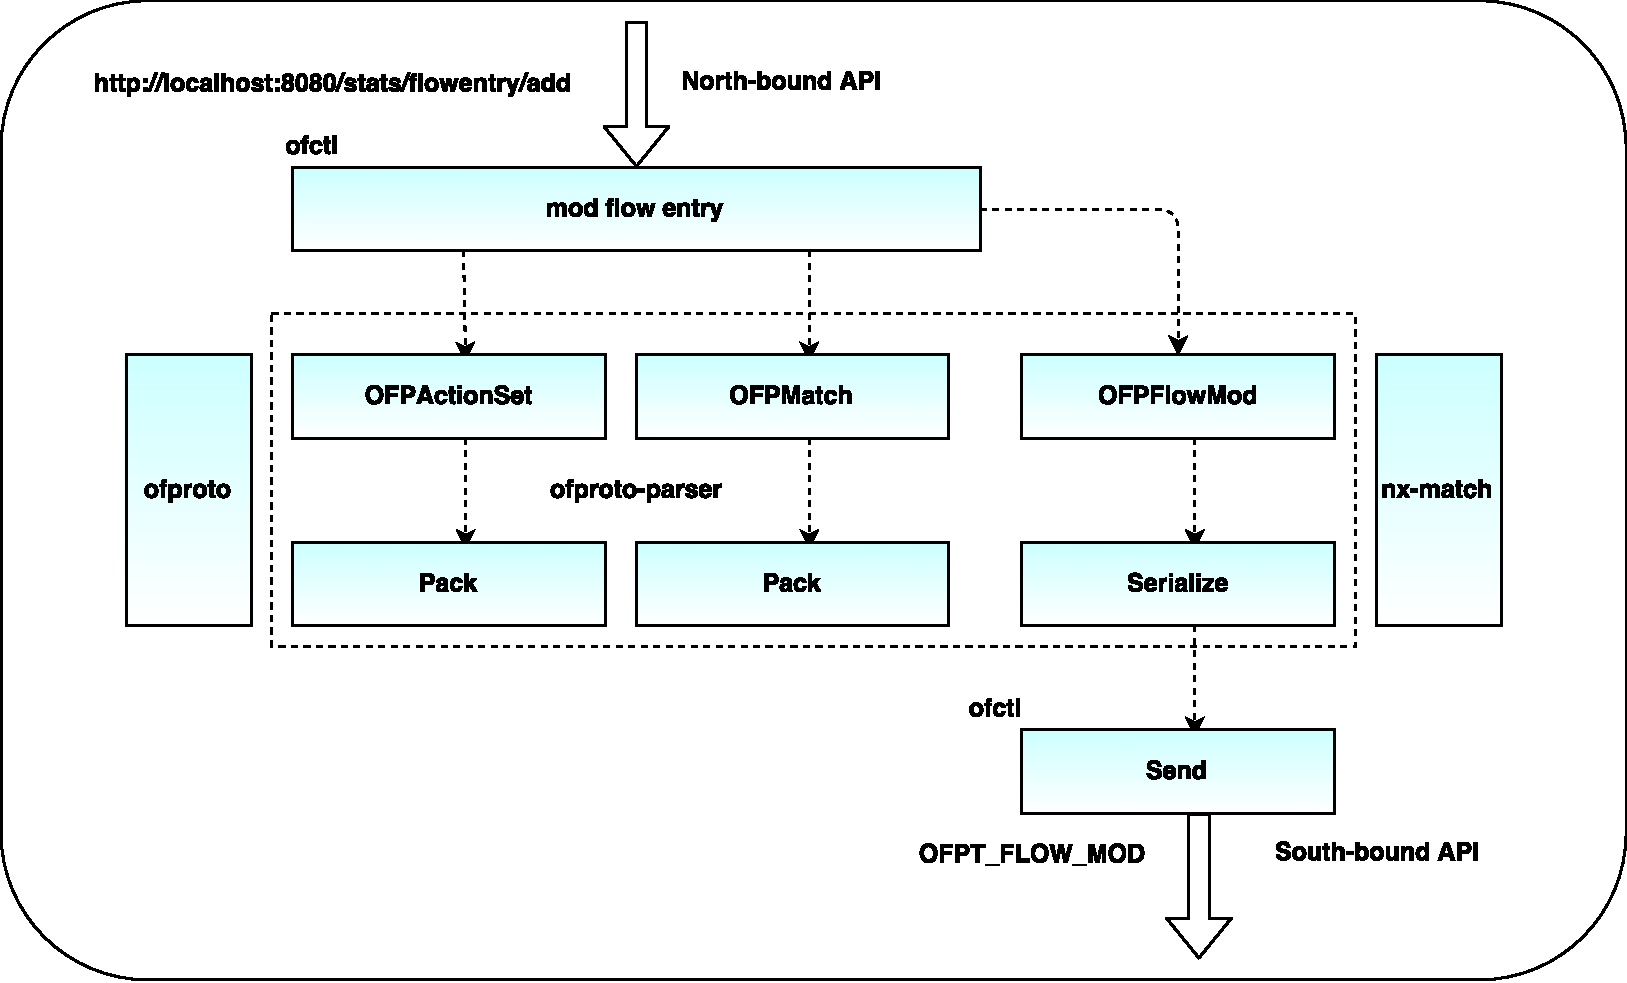
\includegraphics[height=9cm,width=12cm]{ryu01.pdf}
\end{figure}
The implementation is broken down into four parts:
\begin{itemize}
 \item \textbf{ofproto}: In the ofproto module all the event related fields are initialized, and their positions in the OpenFlow message is set. The position set in this module mirror the Open vSwitch support for the event fields. In addition to this, the ofproto module also defines the packing structure the flow-mod message sent to Open vSwitch. In the below snippet, the mapping of event fields and actions between the controller and Open vSwitch is shown. \newline
 
 \begin{lstlisting}[language=python]
 _OFP_MATCH_PACK_STR = 'IH' + OFP_ETH_ALEN_STR + 's' + OFP_ETH_ALEN_STR + \
 'sHBxHBB2xIIHHQQQQ' 
 
 OFPAT_SET_WIN_MAX = 12  # window moving max value for attribute1.
 OFPAT_SET_MOV_MAX = 13  # moving max value for attribute1.
 OFPAT_SET_MIN = 14      # min value for attribute1.
 OFPAT_SET_MAX = 15      # moving max value for attribute1.
 OFPAT_SET_WIN = 16      # window value
 OFPAT_SET_CMP = 17      # compare mode
 
 OFPFW_EVNT_ATTR1 = 1 << 22
 OFPFW_EVNT_ATTR2 = 1 << 23
 OFPFW_EVNT_TYP = 1 << 24
 \end{lstlisting}
 
 \begin{lstlisting}[language=c]
 struct ofpact_map of10[] = {
 ..
 { OFPACT_SET_WIN_MAX, 12},
 { OFPACT_SET_MOV_MAX, 13},
 { OFPACT_SET_MIN, 14},
 { OFPACT_SET_MAX, 15},
 { OFPACT_SET_WIN, 16},
 { OFPACT_SET_CMP, 17}
 ..
 }
 enum ofp10_flow_wildcards {
 ..
 OFPFW10_EVNT_ATTR1 = 1 << 22,
 OFPFW10_EVNT_ATTR2 = 1 << 23,
 OFPFW10_EVNT_TYP   = 1 << 24,
 } 
 \end{lstlisting}
 \item \textbf{nx-match}: In the nx-match module, the methods to serialize the match structure is defined with methods to put each event fields and the respective wild cards into the defined header fields This module takes care of the serialization of the match fields and their wildcards. In the below snippet, the serialization process is show for the event type field. \newline
 
 \begin{lstlisting}[language=python]

 @_register_make
 @_set_nxm_headers([ofproto_v1_0.NXM_OF_EVNT_TYP])
 class MFEVNTTYP(MFField):
 @classmethod
 def make(cls, header):
 LOG.debug('VLOG in point 76')
 return cls(header, MF_PACK_STRING_BE16)
 
 def put(self, buf, offset, rule):
 LOG.debug('VLOG in point 86')
 return self.putm(buf, offset, rule.flow.e_type, rule.wc.e_type_mask)
 
 def serialize_nxm_match(rule, buf, offset):
 if rule.flow.e_type != 0:
 if rule.flow.nw_proto == 17 and rule.wc.e_type_mask == UINT64_MAX:
 header = ofproto_v1_0.NXM_OF_EVNT_TYP
 else:
 header = 0
 if header != 0: 
 offset += nxm_put(buf, offset, header, rule)
 \end{lstlisting}

 \item \textbf{ofctl}: The ofctl module consists of the implementation for the \textit{mod_flow_entry} method which handles the north-bound HTTP enabled flowadd API. In this module, the event fields and actions are extracted from the JSON messages, reads them to previously defined match fields which are sent to the ofproto parser module to pack them into the desired format. \newline
 \begin{lstlisting}
 #read from JSON into e_type string:value pair
  match = dp.ofproto_parser.OFPMatch(wildcards,.. e_type,..) #call OFPMatch
 
 #read from json into set_max string:value pair
 elif action_type == 'SET_MAX':
 val = int(a.get('val', 0))
 actions.append(dp.ofproto_parser.OFPActionSetMax(val))  #call OFPActionSet
 \end{lstlisting}

 \item \textbf{ofproto-parser}: The ofproto-parser module is modified to taking the match and action strings containing event related messages and convert them into Flow and Action structures supporting the relevant event fields and actions. The ofproto-parser module packs relevant structures using the definition provided in the ofproto module and then serializes the message using the methods provided in nx-match modules. The message sent out to the Open vSwitch is a \textit{OFPT_FLOW_MOD} message which is defined in position 14 within the Open vSwitch and hence is packed similarly in RYU. \newline
  \begin{lstlisting}[language=python]
  OFPT_FLOW_MOD = 14       # Controller/switch message
     \end{lstlisting}
     
     In Open vSwitch:
     \begin{lstlisting}[language=c]
  enum ofpraw { 
  /* OFPT 1.0 (14): struct ofp10_flow_mod, uint8_t[8][]. */
  OFPRAW_OFPT10_FLOW_MOD}
  \end{lstlisting}
  
  The below snippet shows the methods added to parse and serialize individual event \textit{set_min} action. \newline 
  
 \begin{lstlisting}[language=python]
 class OFPActionAttrVal(OFPAction):
 def __init__(self, val):
  super(OFPActionAttrVal, self).__init__()
  self.val = val

 @classmethod
 def parser(cls, buf, offset):
  type_, len_, val = struct.unpack_from(
  ofproto.OFP_ACTION_ATTR_VAL_STR, buf, offset)
  assert type_ in (..,
  ofproto.OFPAT_SET_MIN,
  ..)
  assert len_ == ofproto.OFP_ACTION_ATTR_VAL_SIZE
  return cls(val)
 
 def serialize(self, buf, offset):
  msg_pack_into(ofproto.OFP_ACTION_ATTR_VAL_STR,
  buf, offset, self.type, self.len, self.val) 
 
 
 @OFPAction.register_action_type(ofproto.OFPAT_SET_MIN,
 ofproto.OFP_ACTION_ATTR_VAL_SIZE) 
 \end{lstlisting} 

\end{itemize}

\subsubsection{Enable Northbound API}
In addition to changes in the different modules, the Northbound API support is provided to the RYU application by mapping the /flowentry/add command to the mod_flow_entry method within ofctl. The format of the JSON and the usage to add event-based rules into the Open vSwitch is discussed in detail along with examples in the next chapter. \newline


\begin{lstlisting}[language=python]
uri = path + '/flowentry/{cmd}'
mapper.connect('stats', uri,
controller=StatsController, action='mod_flow_entry',
conditions=dict(method=['POST']))
\end{lstlisting}


\section{Summary}
In this chapter, the design and implementation of a programmable event processing framework within Open vSwitch with the RYU controller used as the rules engine was presented. The chapter characterized the goal of the thesis, presented a design breakdown and depicted a system model for events. Three classes of event semantics were expressed within the system model after which the steps taken to implement the system was recounted with necessary illustrations of data flow and snippets of code necessary for fair representation. In the next chapter, the evaluation of the system across several parameters is chronicled with a brief discussion of relevant results.


	\chapter{Evaluation and Results}
In this chapter, the \ac{evs} bridge is evaluated for performance and function. The chapter describes the modes of deployment used for evaluation and the baselines used for measurement and comparison. Wherever eligible a brief discussion of the result is provided with necessary parameters. 


\section{Evaluation Environment}
In Table 5.1, the components working together to form the evaluation environment are listed. At the core of the set up is an Open vSwitch built from the tree with release tag 2.6.1 accelerated by Intel Data Plane Development Kit built from the source with release tag 16.11.2. The hypervisor support comes from Linux-KVM with QEMU 2.9.0 for emulation, running on an Intel(R) Xeon x86_64 CPU with 16 cores. The operating system used is Ubunutu xenial 16.04.2 LTS running a 4.4.0.79-generic kernel. 
\begin{center}
 \captionof{table}{Evaluation Environment} \label{tab:title} 
 \begin{tabular}{ |c|c| } 
  \hline
  Processor &  Intel(R) Xeon(R) CPU E5-2630 v3 @ 2.40GHz  \\
  \hline 
  Architecture &  x86_64  \\ 
  \hline
  CPU(s) & 16  \\ 
  \hline
  Kernel & 4.4.0.79-generic \\
  \hline
  Distribution & Ubuntu xenial 16.04.2 LTS \\
  \hline
  Open vSwitch & 2.6.1 \\
  \hline
  Intel DPDK & 16.11.2 \\
  \hline
  Qemu & Qemu Emulator 2.9.0 \\
  \hline
  Ryu & 4.0 \\
  \hline  
 \end{tabular}
\end{center}

\section{System under Test}
The system under test during the evaluation is the EVS bridge. Firstly the performance of the EVS bridge is measured in terms of link bandwitdh and average round trip time and compared with that of a standard OVS bridge. This is important because an addition of functionality to the OVS bridge should not result in a performance degradation that will make the OVS bridge unusable for the generic switching scenarios it was originally designed for. 
\newline
Secondly, the EVS bridge is evaluated with respect to the problem statement - described in Chapter 1.2 - that there is a performance gain to be attained when aspects of event processing are offloaded on to the underlying network. To evaluate the performance, an  application(evntsrc) is implemented to generate events, and another application(evntsink) is developed to consume the packets and measure latency. Standard packet generators cannot be used for evaluation because of the need to control the format of the packet payload. Performance of the EVS bridge is compared against a custom light-weight userspace application(evntbroker) emulating an event processing engine. The evntbroker application bridged on the standard OVS. The flow-path of data in the two systems is captured in figure 5.1. We can see that EVS bridge replaces the udpbroker and reduces the number of packets in the system. Although the evntbroker does not preform the role of full-fledged complex event processing engine, it is sufficient to provide a baseline for the event processing operations built in to the EVS bridge. The point-to-point latency between evntsrc and evntsink is measured in both the systems- under two deployment scenarios - and the results discussed.

 \begin{figure}[H]    
 \caption{Data Flow in EVS vs OVS}
  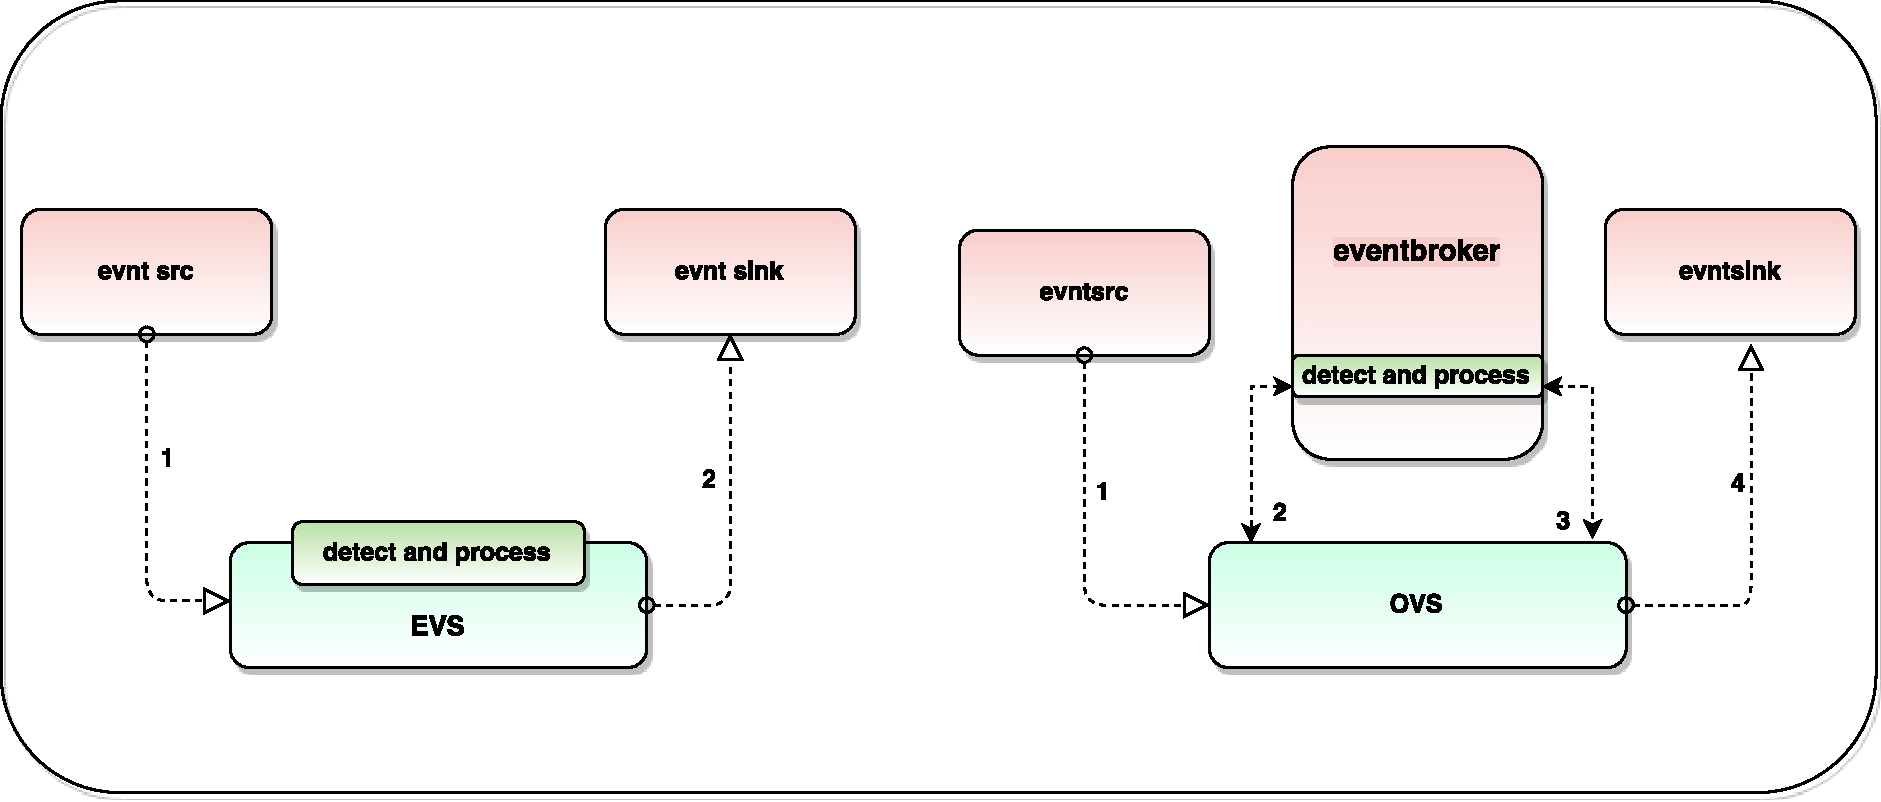
\includegraphics[height=7cm]{evsovs.pdf}
\end{figure}



Thirdly, we measure the performance of the EVS bridge for the following additional parameters:
\begin{itemize}
 \item Measure of latency with increasing size of event types.
 \item Measure of latency with increasing number of event types.
 \item Measure of latency with increasing percentage of filtered flows.
 \item Measure of latency with increasing number of matched event attributes. 
 \item Measure of latency with event attributes detection and redirection.
 \item Measure of latency with compare operations performed on event attributes.
 \item Measure of latency with stateful operations performed on event attributes.
 \item Evaluation of compare operations for accuracy.
 \item Evaluation of stateful operations for accuracy.
\end{itemize}

The Evaluation is performed in two deployment modes:
\begin{itemize}
 \item Network Namespaces: As discussed in Chapter 3.7, a network namespace is a logically separate network stack on the same host machine. Since each namespace has its network stack and can be attached to virtual Ethernet or physical ports, they offer a perfect development environment for Open vSwitch. During the evaluation phase, namespaces were bridged on Open vSwitch using TAP devices. The set-up, methodology, and results are discussed in detail in section 5.4
 \item Qemu-KVM Guests: As discussed in Chapter 3.8, Qemu-KVM provides a combination of device emulation and virtual machine monitoring to set up guest virtual machines on a physical host. The evaluation set up involves Open vSwitch accelerated by Intel DPDK as a hypervisor switch bridging QEMU-KVM guests. The set-up, methodology, and results are discussed in detail in section 5.5.
\end{itemize}


\section{Apparatus for Evaluation}
As briefly discussed in the previous chapter 5.2 and illustrated in figure 5.1, the three components needed for the evaluation are:
\begin{itemize}
 \item Event Source: The EVS bridge implementation handles events only if the packets have a custom tag in the packet. All other packets without the tag are sent through the standard processing flow. Once the tag is detected, the EVS bridge parses the packet payload to derive the event types and event attributes. Hence the packets have to follow the  format \textit{[tag,event_type,event_attribute1,event_attribute2]}. To this end, a Java-based Event Source generator, \textit{evntsrc}, has been implemented to generate \ac{udp} packets in the established format.
  
 \item Event Sink: The events are consumed by an event sink which is responsible for measuring the point to point latency from source to sink. The \textit{evntsink} application has been implemented to consume events and measure the latency.
 
 \item Event Broker: A custom event broker, \textit{evntbroker}, is implemented to perform the operations built-in to the EVS bridge. The evntbroker provides an alternate flow-path for events to that of the flow-path in the EVS bridge. And the flow-path of data is similar to that of any event processing engine. Hence the flow-path provided by evntbroker is referred to as a baseline for evaluation.
\end{itemize}

\section{Evaluation on Network Namespaces}
In this section, we evaluate the performance of userspace-EVS against userspace-OVS. As described in Chapter 5.3, EVS bridge set-up does not include an evntbroker, whereas the standard OVS set-up includes a evntbroker. This is because EVS bridge is equipped to perform the operations of the evntbroker. Figure 5.2 illustrates the set-up for network namespaces. The namespaces are connected to the vSwitch(EVS or OVS) using a pair of virtual Ethernet interfaces. The evntsrc, evntsink, and evntbroker applications are all running in their L3 network namespace. More about the set up of veth-pairs, the format and rate of the generated UDP packets, and the API signatures used to deploy relevant event processing rules are discussed in subsection 5.4.1.

 \begin{figure}[H]
 \centering
 \caption{Namespaces on EVS/OVS}
 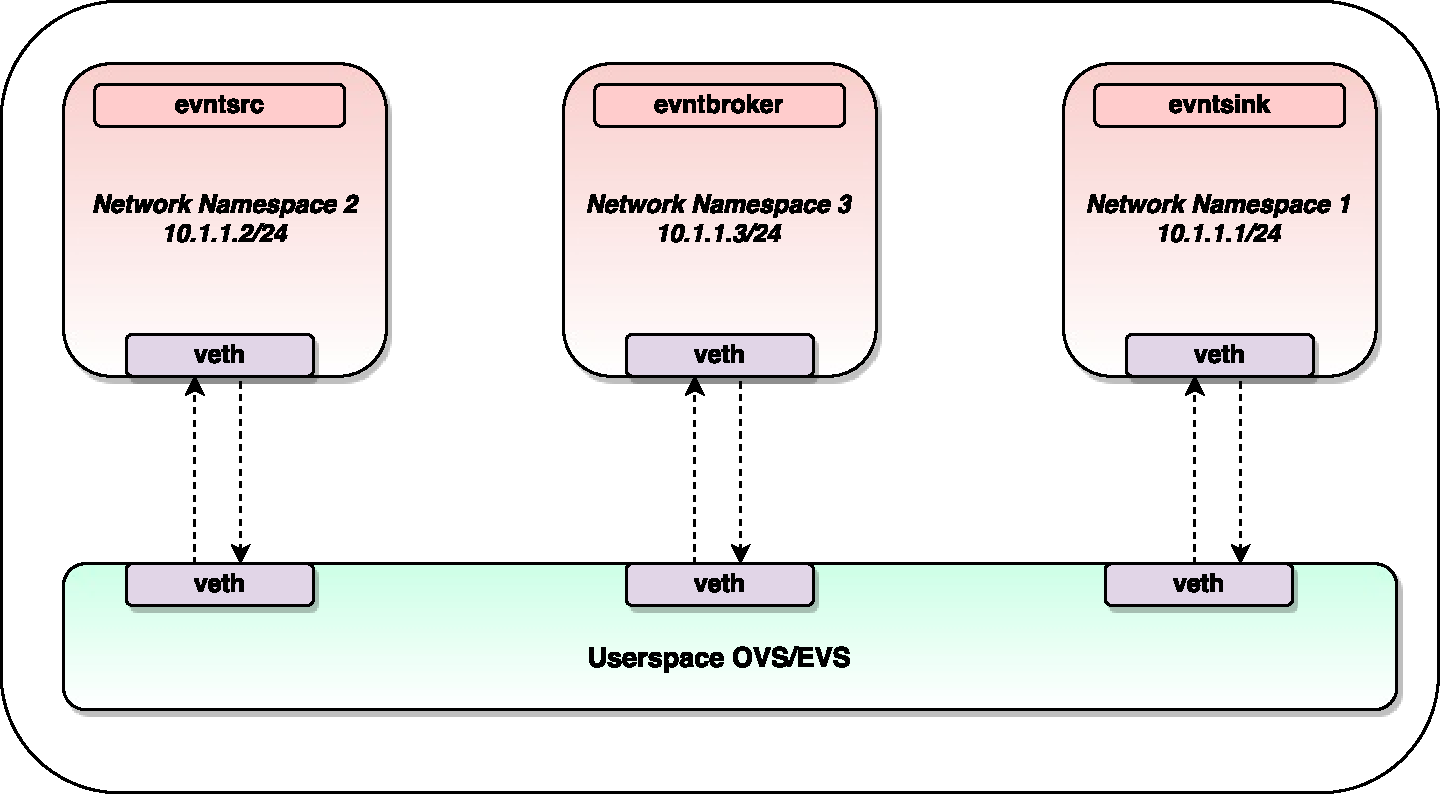
\includegraphics[height=8cm,width=12cm]{nsovs01.pdf}
\end{figure}


\subsection{Set-up Methodology}
In this subsection the steps taken to set up the Network Namespaces bridged on the two userspace bridges is detailed. To begin the set up, it is assumed that the EVS code base is compiled and the ovs-vswitchd daemon and the ovsdb-server are up and running. In addition the modified RYU controler is also running with OpenFlow v1.0.  With this in place, the following steps are taken to set-up the system.
\begin{itemize}
\item To begin the set up, the userspace EVS bridge has to be initialized. \noindent See the following command:
 \begin{lstlisting}[language=bash]
 $ ovs-vsctl add-br br0 -- set bridge br0 datapath_type=netdev \end{lstlisting}
\end{itemize}
\begin{itemize}
 \item The namespaces are set up. In this document, the set up for one namespace is shown.
 \begin{lstlisting}[language=bash]
 $ ip netns add ns1 \end{lstlisting}
\end{itemize}
\begin{itemize}
 \item Two veth pairs of ports are created.
 \begin{lstlisting}[language=bash]
 $ ip link add tap1 type veth peer name ovs-tap1 \end{lstlisting}
\end{itemize}
\begin{itemize}
 \item One end of the created pair is attached to the EVS bridge.
 \begin{lstlisting}[language=bash]
 $ ovs-vsctl add-port br0 ovs-tap1 \end{lstlisting}
\end{itemize}
\begin{itemize}
 \item The other end of the pair is attached to the network namespace.
 \begin{lstlisting}[language=bash]
 $ ip link set tap1 netns ns1 \end{lstlisting}
\end{itemize}
\begin{itemize}
 \item The interface in the network namespace is statically assigned with an ip and both the ends of the pairs are brought up.
 \begin{lstlisting}[language=bash]
 $ ip netns exec ns1 ip link set dev tap1 up
 $ ip netns exec ns1 ip addr add 10.1.1.1/24 dev tap1
 $ ip netns exec ns1 ip link set lo up
 $ ip link set dev ovs-tap1 up \end{lstlisting}
\end{itemize}
\begin{itemize}
 \item The evntsink, evntsrc and evntbroker applications are run on the three namespaces.
 \begin{lstlisting}[language=bash]
 $ ip netns exec ns1 java evntsink
 $ ip netns exec ns2 java evntsrc
 $ ip netns exec ns2 java evntbroker \end{lstlisting}
\end{itemize}

\begin{itemize}
 \item Install the rules onto the EVS bridge to handle the event operations. The API signature for detecting and event of type 'TEST' and redirecting it the evntsink at 10.1.1.1 is shown below:
\begin{lstlisting}[language=json,firstnumber=1]
 {
"dpid": 178974088016461,
"table_id": 0,
"priority": 11112,
"flags": 1,
"match":{
"dl_type":0x0800,
"nw_proto":17,
"nw_dst":"10.1.1.1",
"tp_dst":9877,
"e_type":"TEST"
},
"actions":[{
"type":"set_nw_dst",
"nw_src": 10.1.1.2
"nw_dst": 10.1.1.1
},
{
"type":"NORMAL"
}
]
}
http://localhost:8080/stats/flowentry/add \end{lstlisting}
\end{itemize}

The latency measurements are produced at the evntsink application. It is important to understand the methodology for measurement. Network namespaces are purely separate logical networks. They run on the same CPU and use the Hardware. Technologies such as dockers, Linux containers combine facilities provided by network namespaces, process namespaces, file system namespace, \ac{ipc} namespaces among others with Linux control groups to provide virtualization containers. But network namespaces simply provide a logical network stack. To measure the latency, the evntsrc application sends the system timestamp in the payload. The payload follows the format specified in figure 4.5. On receiving the packet, the eventsink extracts the timestamp from the payload computes the difference between current system time. The delta value is aggregated for 1000 UDP packets in each run to give one trial reading of the point-to-point latency. The same methodology is used in all experiments.

\subsection{Performance measurement without event operations}
In this subsection, the evaluation of latency between the evntsrc and evntsink connected without performing any event detection and redirection operation is detailed. Here the EVS bridge performs the role of a standard OVS bridge because no rules specific to events are installed. The packets are sent directly from evntsrc to evntsink without the need for evntbroker. The same exercise is repeated for the standard OVS bridge in order to contrast the performance of the two bridges. The observed results of this analysis are summarized in Figure 5.4. As we can see, the point-to-point latency between evntsrc and evntsink on the EVS bridge is only slightly greater than that of the point-to-point latency of the same on the standard OVS bridge. The slight increase in latency can be attributed to the fact that the EVS bridge performs deep packet inspection per packet to parse and de-serialize the payload data. 
\newline
In addition to point-to-point latency, the bandwidth of the link, and average \ac{rtt} is measured for both EVS and OVS bridge. To measure the bandwidth of the link, \textit{hperf3} is used and to measure RTT \textit{hping3} is used. As we see in Figure 5.1, EVS bridge is similar to the standard OVS bridge when compared on the parameters of link bandwith and RTT. The bandwidth of the link is  low in both  cases because namespaces are bridged using virtual interfaces and expectedly have low throughput.
\begin{figure}[H]
\centering
\caption{Performance of bridged namespaces}
\begin{tikzpicture} [baseline=(current axis.outer east)]
\begin{axis}[
width=0.5\textwidth,
xlabel={Trial},
ylabel={Point-to-Point Latency(ms)},
xmin=1, xmax=10,
ymin=0.00, ymax=0.30,
xtick={1,2,3,4,5,6,7,8,9,10},
ytick={0,0,05,0.10,0.15,0.20,0.25,0.30},
legend pos=north west,
ymajorgrids=true,
grid style=dashed,
]
\addplot[
color=red,
mark=square,
]
coordinates {
 (1,0.1546)(2,0.1348)(3,0.1464)(4,0.158)(5,0.1396)(6,0.1588)(7,0.144)(8,0.1396)(9,0.1424)(10,0.159)
};
\addlegendentry{EVS - Avg 0.148ms}
\addplot[
color=green,
mark=square,
]
coordinates {
 (1,0.137)(2,0.1456)(3,0.1273)(4,0.1234)(5,0.1269)(6,0.1368)(7,0.1468)(8,0.1434)(9,0.1380)(10,0.1510)
};
\addlegendentry{OVS - Avg 0.137ms}



\end{axis}
\end{tikzpicture}\hfill
 \begin{tabular} {lrr}
 \toprule
 \hline
 &  OVS Bridge & EVS Bridge  \\ \midrule
 \hline 
 Bandwidth &  154 Mbits/s & 149 Mbits/s  \\ 
 \hline
 Avg RTT & 0.183 ms & 0.180 ms  \\ \bottomrule
 \hline 
\end{tabular}
\end{figure}


\subsection{Performance measurement with event detection and redirection}
In this subsection, the performance evaluation of the bridge while performing an event detection and redirection operation on a single event type is presented.  For example, Let us say an event with type 'TEST' is sent from evntsrc to the evntbroker. 
This operation is denoted as: \begin{equation} D(e.t) \quad | \quad stream,  \end{equation}
where \textit{D} is the detect operation; \newline
\textit{|} denotes the redirect operation; \newline
and \textit{stream} is the logical stream to which the detected event is redirected to. \newline \newline

Whereas other streaming applications may have named stream support, EVS stream redirection is done based on network addresses of the application consuming the event stream. The controller rule installed in EVS corresponding to this operation is:

\begin{lstlisting}[language=json,firstnumber=1]
{
"dpid": 178974088016461,
"table_id": 0,
"priority": 11112,
"flags": 1,
"match":{
"dl_type":0x0800,
"nw_proto":17,\\
"nw_src":"10.1.1.2",
"nw_dst":"10.1.1.3",
"tp_dst":9877,
"e_type":"TEST",
},
"actions":[{
"type":"set_nw_dst",
"nw_dst": 10.1.1.1
},
{
"type":"NORMAL"
}
]
}
http://localhost:8080/stats/flowentry/add \end{lstlisting}

Consider a stream of TEST events where each event has readings from multiple sensors which have to be redirected to another processing engine specifically built for handling these events using an Event Processing Language. Such a query is in essence similar to the operation defined in (5.1) and would normally look like:

\begin{verbatim}
INSERT INTO NEWTESTPSTREAM
SELECT * FROM TESTSTREAM
\end{verbatim}

In the EVS bridge, this event of type 'TEST' is detected and redirected to the evntsink using \textit{mod_nw_dst} action rules. Hence the event doesn't go to the evntbroker when EVS bridge is used. As discussed before streams in EVS are identified using network addresses. Named stream support isn't provided. Although it is possible to create custom actions with custom names and make them perform the \textit{mod_nw_dst} actions, in a way mimicking the idea of 'named' streams, this would make a) add more lines of code in the already strong 0.5 million lines of code in OVS, and b) would mean custom action for every stream and thus wouldn't scale.

\begin{figure}[H]
\centering
\caption{Performance of Event Redirection}
\begin{tikzpicture}
\begin{axis}[
xlabel={Trial},
ylabel={Point-to-Point Latency(ms)},
xmin=1, xmax=25,
ymin=0.00, ymax=0.60,
xtick={1,3,5,7,9,11,13,15,17,19,21,23,25},
ytick={0.00,0.10,0.20,0.30,0.40,0.50,0.60},
legend pos=north west,
ymajorgrids=true,
grid style=dashed,
]

\addplot[
color=green,
mark=square,
]
coordinates {
(1,0.27)
(2,0.279)
(3,0.269)
(4,0.227)
(5,0.285)
(6,0.265)
(7,0.26)
(8,0.227)
(9,0.34)
(10,0.288)
(11,0.257)
(12,0.27)
(13,0.28)
(14,0.24)
(15,0.28)
(16,0.27)
(17,0.28)
(18,0.27)
(19,0.26)
(20,0.3)
(21,0.24)
(22,0.248)
(23,0.32)
(24,0.28)
(25,0.22)
 
};
\addlegendentry{OVS : Avg 0.269 ms}

\addplot[
color=red,
mark=square,
]
coordinates {
 (1,0.31)
 (2,0.305)
 (3,0.272)
 (4,0.297)
 (5,0.313)
 (6,0.313)
 (7,0.308)
 (8,0.288)
 (9,0.311)
 (10,0.305)
 (11,0.3)
 (12,0.317)
 (13,0.312)
 (14,0.3)
 (15,0.299)
 (16,0.309)
 (17,0.306)
 (18,0.308)
 (19,0.31)
 (20,0.297)
 (21,0.286)
 (22,0.306)
 (23,0.281)
 (24,0.306)
 (25,0.318)
 
};
\addlegendentry{EVS : Avg 0.303 ms}

\addplot[
color=blue,
mark=square,
]
coordinates {
 (1,0.348)
 (2,0.343)
 (3,0.316)
 (4,0.327)
 (5,0.296)
 (6,0.338)
 (7,0.346)
 (8,0.33)
 (9,0.335)
 (10,0.355)
 (11,0.335)
 (12,0.327)
 (13,0.327)
 (14,0.318)
 (15,0.347)
 (16,0.314)
 (17,0.304)
 (18,0.301)
 (19,0.33)
 (20,0.288)
 (21,0.339)
 (22,0.326)
 (23,0.31)
 (24,0.309)
 (25,0.281)
 
};
\addlegendentry{EVS-broker: Avg 0.324 ms}

\end{axis}
\end{tikzpicture}
\end{figure}

The same experiment is repeated on the OVS bridge. But in this case, the event with type 'TEST' is simply forwarded to the evntbroker, which proceeds to detect the event and sends it to the relevant evntsink. As we can see in the graph in figure 5.5, the performance of event redirection at the EVS bridge is lower than the performance of event redirection done on an evntbroker, albeit marginally. Even though the EVS bridge prevents the packet from going into the evntbroker and reduces the number of hops for the event packet, the expected improvement in performance is not seen. This can be explained by two factors. One, the redirection in EVS bridge is performed by \textit{mod_tp_dst} or \textit{mod_nw_dst} or \textit{mod_dl_dst} depending on the layer. These OpenFlow actions modify the event packet and also redirect the individual event packet into the datapath interface, which in the case of userspace EVS is dpif-netdev. This additional parsing and lookup balances out the benefits of removing the evntbroker. Two, the EVS bridge employs per packet event deserialization and parsing, which adds some overhead. 

In addition to the above-described experiments, the EVS bridge was set up with an evntbroker and evaluated to get a better sense of the performance. In this set up although the EVS bridge is used, the event detection rules are not installed. Instead, the events are forwarded to the broker as if operating in the standard OVS mode. These results show far higher latency than the standard OVS bridge and slightly higher latency compared to the EVS bridge running in event processing mode. In the latter case, EVS in event processing mode has two fewer packet hops resulting in lower latency. In the former case, we see that although the OVS bridge and EVS in evntbroker have an equal number of packet hops, the per-packet parsing and de-serialization of events, as described before, add an overhead. By comparing the three results, we get an idea of how much overhead is added by the per-packet event parsing and de-serialization and how much overhead is added by the context switch and the extra packet hops. 

These results provide an interesting insight into the evaluation process in a virtualized environment. In a virtualized environment the costs added by the per-packet processing are going to be similar to the per-packet processing overhead in namespaces, but the costs added by context switch from host to VM, back to host are going to be a lot more expensive. There is more discussion on this topic in section 5.5.

\subsection{Performance measurement with increasing size of event types}
In this subsection, an evaluation of the bridge is presented with an increasing size of event types. To do the same, the evntsrc generates events with types ranging from 1 to 9 characters. The analysis was done on the EVS bridge and the OVS bridge. As seen in the left graph plotted in Figure 5.6, the increasing size of an event type string doesn't result in a linear increase in latency in both the cases. For EVS bridge, this is explained by the fact that Tuple search space classifier of Open vSwitch creates a hash table for every unique combination of inserted flow rule. In the case of this evaluation, one flow rule is added for each run, while increasing the size of event type field in consecutive runs. Additionally, although the event type field matches against a string in the event payload, the match field during flow rule insertion for event type is a Hexadecimal value of the string. The rationale behind this approach is that strings within an event payload are serialized into Hexadecimal values on the wire, and since event parsing is part of the packet processing pipeline, keeping the fields, as-is avoids the expensive conversion, thus reducing the overhead on the processing pipeline. 

In the case of the OVS bridge, the broker does a simple string match, and increasing the size of the string makes little to no difference. It would, therefore, be interesting to see how adding additional event types would impact the performance of the two bridges. 

\begin{figure}[H]
 
    \noindent\hrulefill

\noindent
\caption{Changing Size and Number of Event Types}
 \begin{tikzpicture} 
 \begin{axis}[
 xlabel={Size of Event Types},
 ylabel={Point-to-Point Latency(ms)},
 xmin=1, xmax=9,
 ymin=0.00, ymax=0.60,
 xtick={1,2,3,4,5,6,7,8,9},
 ytick={0.00,0.10,0.20,0.30,0.40,0.50,0.60},
 legend pos=north west,
 ymajorgrids=true,
 grid style=dashed,
 ]
 \addplot[
 color=red,
 mark=square,
 ]
 coordinates {
  (1,0.32)(2,0.31)(3,0.28)(4,0.27)(5,0.32)(6,0.29)(7,0.30)(8,0.32)(9,0.33)
 };
 \addlegendentry{EVS : Avg 0.304ms}
 
  \addplot[
 color=green,
 mark=square,
 ]
 coordinates {
  (1,0.27)(2,0.256)(3,0.28)(4,0.292)(5,0.28)(6,0.256)(7,0.329)(8,0.26)(9,0.28)
 };
 \addlegendentry{OVS : Avg 0.273ms}
 
 \end{axis}
 \end{tikzpicture} 
       \hfil
 \begin{tikzpicture} 
\begin{axis}[
xlabel={Number of Event Types/Rules},
ylabel={Point-to-Point Latency(ms)},
xmin=10, xmax=100,
ymin=0.00, ymax=0.60,
xtick={10,20,30,40,50,60,70,80,90,100},
ytick={0.00,0.10,0.20,0.30,0.40,0.50,0.60},
legend pos=north west,
ymajorgrids=true,
grid style=dashed,
]
\addplot[
color=red,
mark=square,
]
coordinates {
 (10,0.319)(20,0.33)(30,0.32)(40,0.32)(50,0.30)(60,0.30)(70,0.308)(80,0.32)(90,0.31)(100,0.308)
};
\addlegendentry{EVS : Avg 0.3135ms}

\addplot[
color=green,
mark=square,
]
coordinates {
 (10,0.27)(20,0.2795)(30,0.265167)(40,0.259)(50,0.2485)(60,0.309)(70,0.270)(80,0.2887)(90,0.254)(100,0.274)
};
\addlegendentry{OVS Bridge: Avg 0.272ms}

\end{axis}
\end{tikzpicture}
\end{figure} 

\subsection{Performance measurement with increasing number of event types } 
In addition to the size of event types, the number of event types sent to the EVS bridge was also increased to measure the impact on latency. Each event type is handled by one rule in EVS bridge, so to handle 100 event types and redirect them to evntsink the EVS bridge was set up with 100 rules. As seen in the right graph in Figure 5.6, an increase in the number of event types/rules does not affect the performance of the EVS bridge. This is because the number of flow rules remains constant, only the actions on each flow rule are modified to increase filtered events. And since the Tuple Space Search Classifier only adds a hashtable when there is a new combination of fields entered as a flow rule, even increasing the number flow rules, as long as they have the same match fields would not result in additional lookups.
The same two experiment setups were repeated for the standard OVS bridge, with an evntbroker responsible for handling and forwarding the event types to the evntsrc. EVS bridge and OVS bridge performed similarly in this regard showcasing the potential of the EVS bridge in real-world scenarios.



\begin{figure}[H]
 \centering
 \caption{Performance of Event Filtering}
 \begin{tikzpicture}
 \begin{axis}[
 xlabel={Percentage of Events Filtered},
 ylabel={Point-to-Point Latency(ms)},
 xmin=1, xmax=90,
 ymin=0.00, ymax=0.60,
 xtick={10,20,30,40,50,60,70,80,90},
 ytick={0.00,0.10,0.20,0.30,0.40,0.50,0.60},
 legend pos=north west,
 ymajorgrids=true,
 grid style=dashed,
 ]
 \addplot[
 color=red,
 mark=square,
 ]
 coordinates {
  (0,0.308)
  (10,0.31)
  (20,0.32)
  (30,0.29)
  (40,0.32)
  (50,0.29)
  (60,0.32)
  (70,0.32)
  (80,0.33)
  (90,0.34)
 };
 \addlegendentry{EVS : Avg 0.312 ms}
 
 \addplot[
 color=green,
 mark=square,
 ]
 coordinates {
  (0,0.274)
  (10,0.267)
  (20,0.279)
  (30,0.25)
  (40,0.251)
  (50,0.261)
  (60,0.255)
  (70,0.258)
  (80,0.258)
  (90,0.242)
 };
 \addlegendentry{OVS : Avg 0.26 ms}
 
 \end{axis}
 \end{tikzpicture}
\end{figure} 

\subsection{Performance measurement with increasing percentage of filtered event types}
In this subsection, the performance evaluation of the EVS bridge with an increasing percentage of filtered event types is presented. The evntsrc is configured to generate 100 random event types, addressed to the evntbroker. The EVS bridge initially is configured with flow rules to send through all the events. At this stage, the setup is similar to the sub-section 5.4.3 with 100 event types and flow rules. In the next stage, 10\% of the event types are filtered with an additional 10\% added subsequently until all the events are filtered. The same experiment is repeated for the standard OVS bridge. In the case of OVS bridge, the filtering is done in the evntbroker. 
\newline
As seen in the graph plotted in Figure 5.7, both EVS and OVS perform very similarly when the percentage of event filters is increased. This experiment however does not showcase the benefits of event filtering in EVS. Because the measurements are taken only when the event is delivered to the evntsink. And for the event to be delivered to the evntsink, it must first be redirected by the EVS bridge using the expensive \textit{mod} actions. 





\subsection{Performance measurement of event attributes detection and redirection}
In this subsection, the performance evaluation of the EVS bridge is presented when event attributes are detected and redirected. The results are contrasted to the measurements produced when similar attributes are detected and redirected using the evntbroker on the OVS bridge. To do the set up for the experiment, rules are installed into the EVS bridge to detect event attributes. When the events with the given attribute or pattern of attributes are detected, the events are redirected to the evntsink. All the other events are filtered out. 

\subsubsection{Detect operation on one attribute}

First, the rule for detecting event type and  a single event attribute is considered. This operation is denoted by: \begin{equation} D(e.t  \wedge e.a_1) \quad | \quad stream,  \end{equation}
where \textit{D} is the detect operation; \newline
\textit{e.t} is the event type; \newline
\textit{e.a1} is the first event attribute; \newline
| denotes the redirect operation; \newline
and \textit{stream} is the logical stream to which the detected event is redirected to. \newline \newline

Whereas other streaming applications may have named stream support, EVS stream redirection is done based on network addresses of the application consuming the event stream. The controller rule installed in EVS corresponding to this operation is:

\begin{lstlisting}[language=json,firstnumber=1]
{
"dpid": 178974088016461,
"table_id": 0,
"priority": 11112,
"flags": 1,
"match":{
"dl_type":0x0800,
"nw_proto":17,
"nw_src":"10.1.1.3"
"nw_dst":"10.1.1.2",
"tp_dst":9877,
"e_type":"TEMP",
"e_attr1":80,
},
"actions":[{
"type":"set_nw_dst",
"nw_dst": 10.1.1.1
},
{
"type":"NORMAL"
}
]
}
http://localhost:8080/stats/flowentry/add \end{lstlisting}

This is similar to the INSERT INTO clause provided by many Event Processing Languages, where the events from an event stream are filtered based on a value and forwarded into another event stream. In this case, the new event stream is the stream of events handed over to the application listening on port 9877. Consider a stream of temperature events where each event has readings from multiple sensors. The operation at (5.2) is semantically similar to the below Event-Processing  query:

\begin{verbatim}
INSERT INTO NEWTEMPSTREAM
SELECT * FROM TEMPSTREAM
WHERE DEVICE_1.VALUE = 80
\end{verbatim}

As seen in Figure 5.8, the latency caused by performance of the operation denoted in (5.2) in the EVS bridge is marginally higher than the latency observed on the standard OVS bridge by order of 0.02 ms. When the same operation was evaluated on the EVS bridge operating in standard mode, the latency observed was marginally higher than the OVS bridge by a order 0.03 ms. This is effectively the latency added by per-packet event processing. 

\pgfplotstableread[row sep=\\,col sep=&]{
 Operations & OVS & EVS & EVS-broker \\
 5.1     & 0.27  & 0.30  & 0.32  \\
 5.2     & 0.27 & 0.29  & 0.313  \\
 5.3    & 0.28 & 0.29 & 0.318 \\
 5.4    & 0.29 & 0.3 & 0.308 \\
}\mydata



\begin{figure}[H]
 \centering
 \caption{Performance of Event attribute match operations}
 \begin{tikzpicture}
 \begin{axis}[
 ybar,
 xlabel={Operations},
 ylabel={Point-to-Point Latency(ms)},
 symbolic x coords={5.1,5.2,5.3,5.4},
    xtick=data,
 nodes near coords,
legend style={at={(0.5,1.0)},anchor=south}, legend columns=-1
 ]
 \addplot[fill=green] table[x=Operations,y=OVS]{\mydata}; \addlegendentry{OVS}
 \addplot[fill=red ] table[x=Operations,y=EVS]{\mydata};  \addlegendentry{EVS}
 \addplot[fill=blue] table[x=Operations,y=EVS-broker]{\mydata}; \addlegendentry{EVS-broker}
    
 \end{axis}
 \end{tikzpicture}
\end{figure}

\subsubsection{Detect operation on two disjunct attributes}

The next operation considered for evaluation is denoted by:

\begin{equation}D(e.t  \wedge (e.a_1 \vee e.a_2)) \quad | \quad stream, \end{equation}
where \textit{D} is the detect operation; \newline
\textit{e.t} is the event type; \newline
\textit{e.a1} is the first event attribute; \newline
\textit{e.a2} is the second event attribute;
| denotes the redirect operation; \newline
and \textit{stream} is the logical stream to which the detected event is redirected to. \newline \newline

The controller installs an additional rule - seen below - in addition to the one above, to perform this operation:
\begin{lstlisting}[language=json,firstnumber=1]
{
"dpid": 178974088016461,
"table_id": 0,
"priority": 11112,
"flags": 1,
"match":{
"dl_type":0x0800,
"nw_proto":17,
"nw_src":"10.1.1.2"
"nw_dst":"10.1.1.3",
"tp_dst":9877,
"e_type":"TEMP",
"e_attr2":80,
},
"actions":[{
"type":"set_nw_dst",
"nw_dst": 10.1.1.1
},
{
"type":"NORMAL"
}
]
}
http://localhost:8080/stats/flowentry/add \end{lstlisting}

Drawing parallel to an Event Processing Language, the operation at (5.2) is similar to:

\begin{verbatim}
INSERT INTO NEWTEMPSTREAM
SELECT * FROM TEMPSTREAM
WHERE DEVICE_1.VALUE = 80 OR DEVICE_2.VALUE=80
\end{verbatim}

As we see in Figure 5.8, the execution of this operation follows the trends observed for operations 5.1 ad 5.2. No remarkable overhead was added on the EVS bridge, despite the addition of the rule. The reason for this is explained in section 5.4.6.


\subsubsection{Detect operation on two conjunct attributes}
The next operation considered for evaluation is denoted by:

\begin{equation}D(e.t  \wedge (e.a_1 \wedge e.a_2)) \quad | \quad stream, \end{equation}
where \textit{D} is the detect operation; \newline
\textit{e.t} is the event type; \newline
\textit{e.a1} is the first event attribute; \newline
\textit{e.a2} is the second event attribute;
| denotes the redirect operation; \newline
and \textit{stream} is the logical stream to which the detected event is redirected to. \newline \newline

The controller installs one rule - seen below - to perform this operation:
\begin{lstlisting}[language=json,firstnumber=1]
{
"dpid": 178974088016461,
"table_id": 0,
"priority": 11112,
"flags": 1,
"match":{
"dl_type":0x0800,
"nw_proto":17,
"nw_src":"10.1.1.2"
"nw_dst":"10.1.1.3",,
"tp_dst":9877,
"e_type":"TEMP",
"e_attr1":80,
"e_attr2":80,
},
"actions":[{
"type":"set_nw_dst",
"nw_dst": 10.1.1.1
},
{
"type":"NORMAL"
}
]
}
http://localhost:8080/stats/flowentry/add \end{lstlisting}

Drawing parallel to an Event Processing Language, the operation at (5.2) is similar to:

\begin{verbatim}
INSERT INTO NEWTEMPSTREAM
SELECT * FROM TEMPSTREAM
WHERE DEVICE_1.VALUE = 80 AND DEVICE_2.VALUE=80
\end{verbatim}

As seen in Figure 5.8, and similar to the case of disjunction operation (5.3), the execution of the conjunction operation in the EVS bridge does not add any remarkable point-to-point latency. And as expected, the EVS-broker has the worst performance, because of the added processing and packet hops.

\subsubsection{Network Traffic Monitoring for the event detection and redirection operations}
For all the operations defined through 5.1 to 5.4, the traffic in the network was monitored both in the case of OVS and EVS bridge. The system was set up to send a flow of 100000 UDP packets from the eventsrc to the evntsink. The traffic characteristics observed on the six interfaces are shown in Table 5.2. It can be observed that the EVS bridge avoids using the interfaces related to namespace 3 completely for the flow. That is a 33\% reduction in traffic for single staged event processing.

\begin{center}
 \captionof{table}{Network traffic on Namespaces} \label{tab:title} 
 \begin{tabular}{ |c|c|c| }
  \hline
   \textbf{Interface} &  \textbf{OVS Bridg}e &  \textbf{EVS Bridge} \\\toprule
  \hline
  Hypervisor - tap1 & Tx-100000 & Tx-100000  \\
  \hline 
  Namespace1 - tap1 & Rx-100000 & Rx-100000 \\
  \hline  
  Hypervisor - tap2 &  Rx-100000 & Rx-100000  \\ 
  \hline
  Namespace2 - tap2 & Tx-100000 & Tx-100000 \\
  \hline  
  Hypervisor - tap3 & Rx-100000, Tx-100000 & 0  \\ 
  \hline
  Namespace3 - tap3 & Rx-100000, Tx-100000 & 0 \\
  \hline
 \end{tabular}
\end{center}


\subsection{Performance measurement of compare operations on event attributes}
In this subsection, the performance of the comparison operations on the event attributes is presented. This class of operations performs a binary operation on the event attribute value. The evaluation of two compare operators who have been implemented- \textit{Greater than or equal to (>=)}, \textit{Less than or equal to (<=)} - is detailed. 

\subsubsection{Greater than or equal to operator}
The operation supported by Greater than or equal to operator is denoted by:
\begin{equation}D(e.t  \wedge (e.a_1 >= value) \quad | \quad filter, \end{equation}
where \textit{D} is the detect operation; \newline
\textit{e.t} is the event type; \newline
\textit{e.a1} is the first event attribute; \newline
\textit{value} is the integer value to be compared with; \newline
| denotes the redirect operation; \newline
and \textit{fliter} is the denotation for filtering of the event. \newline \newline
\begin{lstlisting}[language=json,firstnumber=1]
{
 "dpid": 178974088016461,
 "table_id": 0,
 "priority": 11112,
 "flags": 1,
 "match":{
  "dl_type":0x0800,
  "nw_proto":17,
  "nw_src":"10.1.1.2",
  "nw_dst":"10.1.1.1",
  "tp_dst":9877,
  "e_type":"TEMP",
 },
 "actions":[{
  "type":"SET_MAX",
  "value": 100
 }

 ]
}
http://localhost:8080/stats/flowentry/add \end{lstlisting}

Which in the perspective of event query languages can be represented as:

\begin{verbatim}
DROP FROM TEMPSTREAM
WHERE DEVICE_1.VALUE >= 100
\end{verbatim}

The operation at (5.5) can be used with conjunction operation on event attribute2.
\begin{equation}D(e.t  \wedge ((e.a_1 >= value) \wedge e_2 )\quad | \quad filter, \end{equation}

or with the disjunction operation on attribute2.

\begin{equation}D(e.t  \wedge ((e.a_1 >= value) \vee e_2 )\quad | \quad filter, \end{equation}

 The Less than or equal to operator is introduced next, and the evaluation discussion of the two operators is presented together at the end of the subsection.

\subsubsection{Less than or equal to operator}
The operation supported by Greater than or equal to operator is denoted by:
\begin{equation}D(e.t  \wedge (e.a_1 <= value) \quad | \quad filter, \end{equation}
where \textit{D} is the detect operation; \newline
\textit{e.t} is the event type; \newline
\textit{e.a1} is the first event attribute; \newline
\textit{value} is the integer value to be compared with; \newline
| denotes the redirect operation; \newline
and \textit{fliter} is the denotation for filtering of the event. \newline \newline
\begin{lstlisting}[language=json,firstnumber=1]
{
"dpid": 178974088016461,
"table_id": 0,
"priority": 11112,
"flags": 1,
"match":{
"dl_type":0x0800,
"nw_proto":17,
"nw_dst":"10.1.1.2",
"nw_dst":"10.1.1.1",
"tp_dst":9877,
"e_type":"TEMP",
},
"actions":[{
"type":"SET_MIN",
"value": 100
}
]
}
http://localhost:8080/stats/flowentry/add \end{lstlisting}

Which in the perspective of event query languages can be represented as:

\begin{verbatim}
DROP FROM TEMPSTREAM
WHERE DEVICE_1.VALUE <= 100
\end{verbatim}

The operation at (5.8) can be used with conjunction operation on event attribute2.
\begin{equation}D(e.t  \wedge ((e.a_1 <= value) \wedge e_2 )\quad | \quad filter, \end{equation}

or with the disjunction operation on attribute2.

\begin{equation}D(e.t  \wedge ((e.a_1 <= value) \vee e_2 )\quad | \quad filter, \end{equation}

The attr_cmp action defined in section 4.6.7 internal implements the {<,>,=} operators, the performance observed for the set_min, set_max operators can be generalized for the class of compare operations defined in section 4.6.7. Hence For evaluation purposes only the set_min and set_max operators defined in (5.5) and (5.8) are considered. 

\subsubsection{Performance of compare Operations}
In this subsection, the performance of the compare operations defined in section 4.6.7 is presented. First, the evaluation  of rules defined in (5.5) and (5.8) is presented when only positive values are sent to the system. This evaluation is done in order to understand the rule performance is general and to see if the rule in itself creates a bottleneck in performance. For example, for a set_min:100 rule, only events of type "TEMP" and with values greater than 100 are sent. In this case, each event is forwarded by the rule and none of the events are dropped. The same test was repeated for the set_max:100 operator but this time by passing values less than 100. This test is not intended to test the accuracy of the rules, but only to check if the rules with additional operations add an overhead. The performance is plotted in Figure 5.8 and is contrasted with the inter-namespace switching results provided in section 5.4.2, figure 5.4. As it can be seen, the rules for the two operations do not add a significant overhead and are comparable to the performance of the EVS bridge with inter-namespace switching based on event type attribute.
\begin{figure}[H]
 \centering
 \caption{Performance of compare operations}
 \begin{tikzpicture} [baseline=(current axis.outer east)]
 \begin{axis}[
 width=0.5\textwidth,
 xlabel={Trial},
 ylabel={Point-to-Point Latency(ms)},
 xmin=1, xmax=10,
 ymin=0.00, ymax=0.30,
 xtick={1,2,3,4,5,6,7,8,9,10},
 ytick={0.00,0,05,0.10,0.15,0.20,0.25,0.30},
 legend pos=north west,
 ymajorgrids=true,
 grid style=dashed,
 ]
 \addplot[
 color=red,
 mark=square,
 ]
 coordinates {
  (1,0.1546)(2,0.1348)(3,0.1464)(4,0.158)(5,0.1396)(6,0.1588)(7,0.144)(8,0.1396)(9,0.1424)(10,0.159)
 };
 \addlegendentry{EVS - Avg 0.148ms}
 \addplot[
 color=green,
 mark=square,
 ]
 coordinates {
  (1,0.137)(2,0.1456)(3,0.1273)(4,0.1234)(5,0.1269)(6,0.1368)(7,0.1468)(8,0.1434)(9,0.1380)(10,0.1510)
 };
 \addlegendentry{OVS - Avg 0.137ms}
   \addplot[
 color=blue,
 mark=square,
 ]
 coordinates {
  (1,0.1699)(2,0.1453)(3,0.1456)(4,0.1456)(5,0.158)(6,0.147)(7,0.163)(8,0.154)(9,0.142)(10,0.143)
  
 };
 \addlegendentry{EVS - set_max - Avg 0.151ms}
 
 \addplot[
 color=yellow,
 mark=square,
 ]
 coordinates {
  (1,0.153)(2,0.158)(3,0.147)(4,0.16)(5,0.149)(6,0.149)(7,0.143)(8,0.154)(9,0.152)(10,0.16)
 };
 \addlegendentry{EVS - set_min - Avg 0.152ms} 
 
 
 \end{axis}
 \end{tikzpicture}\hfill

\end{figure}


\subsection{Evaluating for accuracy - compare operations}
In the previous subsection, the performance of the comparison operations was measured only with positive test inputs where none of the events are dropped. But when random values are sent as attributes, the compare operations fail to perform the role they are designed for accurately. This is because of the megaflow cache design of the Open vSwitch. The cross product of all the active flows in the userspace OpenFlow tables is cached in the megaflow table. And as long as the incoming flow matches an entry in the megaflow table, the learned action is applied. This makes compare actions tricky to implement. These actions are conditional, i.e., if the expression specified by the action evaluates to TRUE, the forwarding action is applied, or else the drop action (or a lack of action) is applied. So when a set_max:100 actions is evaluated for the first event, the value for event attribute is extracted; for the ease of discussion let us consider 90 to be this value. Therefore, the set_max action evaluates to TRUE, after which the packet is sent to the learned port based on the 'nw_dst' address. This flow is now cached in the megaflow table with the learned output port. Figure 5.9 illustrates the megaflow cache.
\begin{figure}[H]
 \centering
 \caption{Megaflow cache}
 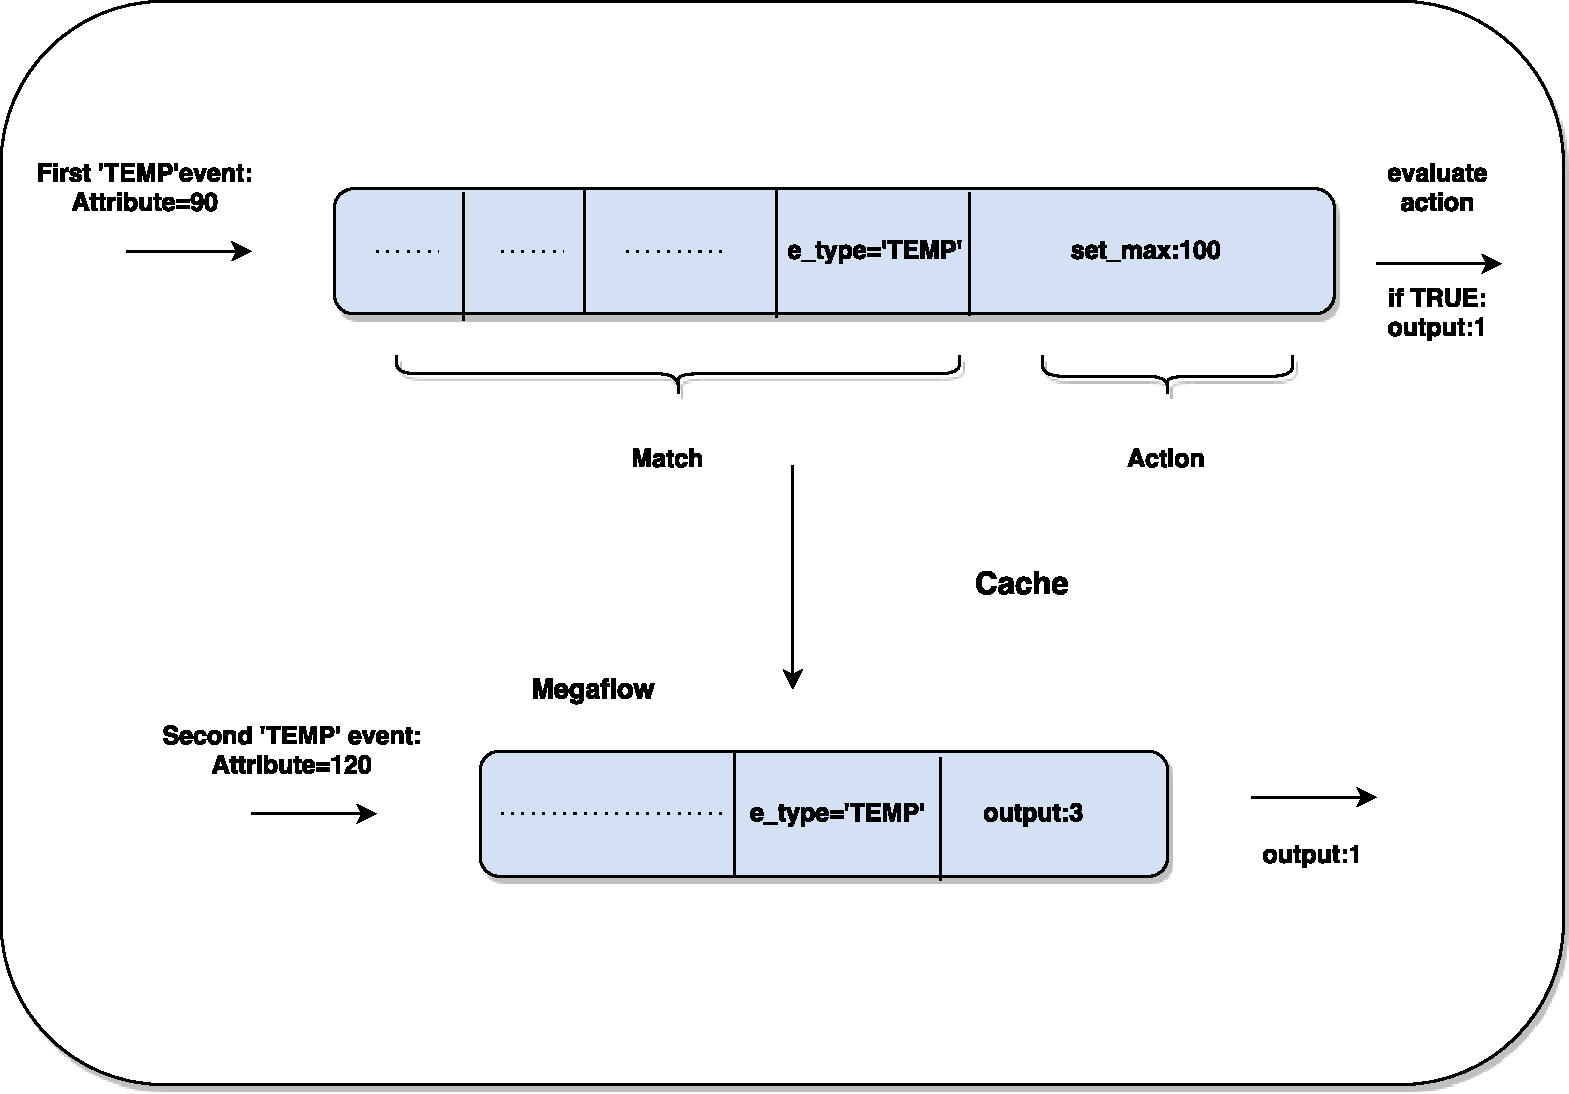
\includegraphics[height=7cm]{learnandcache.pdf}
\end{figure}
The subsequent events are now looked-up in the megaflow cache, and the cached forwarding action is applied. Hence once the events start hitting the megaflow table, there is no opportunity for attribute evaluation. Open vswitch implements a re-validator thread which evicts the inactive flows or to update the recently changed flows. The compare operations from this perspective can be viewed as flows which need to be refreshed after every flow hit. By default, the cache revalidation happens every 10 seconds. So if an event of type 'TEMP' hits the compare operator rule once in 10 seconds, the operation is evaluated accurately. However, this is not ideal. Hence different ways to reduce this flow hit rate are explored. Open vSwitch provides options to configure the revalidation of the cache.\newline

\subparagraph*{Disabled-Megaflow}
The first approach is to disable-megaflow, using the below command.

 \begin{lstlisting}[language=bash]
$ ovs-appctl upcall/disable-megaflows \end{lstlisting}

After having disabled megaflows, the evaluation to determine the accuracy and performance of the compare operations was performed. The rule installed for this evaluation was:

\begin{lstlisting}[language=json,firstnumber=1]
{
"dpid": 178974088016461,
"table_id": 0,
"priority": 11112,
"flags": 1,
"match":{
"dl_type":0x0800,
"nw_proto":17,
"nw_dst":"10.1.1.2",
"nw_dst":"10.1.1.1",
"tp_dst":9877,
"e_type":"TEMP",
},
"actions":[{
"type":"set_max",
"value": 5
},
{
"type":"NORMAL"
}
]
}
http://localhost:8080/stats/flowentry/add \end{lstlisting}

The results are monitored such that only values greater than 5 are filtered by the EVS bridge, and values less than 5 are allowed through. To test this, the evntsrc is configured to generate events of type 'TEMP,' such that every odd iteration generates a value greater than 5 and every even iteration generates a value less than 5. The evntsink counts any unexpected value greater than 5 received as a miss, and reports at the end of the test. 

Another additional parameter that is set up is the frequency of the rule hit. As discussed before, by default Open vSwitch evicts idle megaflow rule every 10 seconds. With the megaflow disabled, this frequency of rule hit was configured by increasing the sleep time of the evntsrc application. This was done to measure the accuracy when the frequency is high. This also gives a good indicator of the frequency of rule hit that can be tolerated while having the highest accuracy. The results are plotted in Figure 5.11


\begin{figure}[H]  
 
 \caption{Accuracy and latency measure of compare operations with disabled megaflows}
 \begin{tikzpicture}
 \begin{axis}[
 xlabel={Delay in rule hit(ms)},
 ylabel={Accuracy of compare operations},
 symbolic x coords={0,5,10,15,20,25},
 xtick=data,
 nodes near coords,
 legend style={at={(0.5,1)},
  anchor=north,legend columns=-1},
 ]
 \addplot[ybar,fill=red] coordinates {
  (0,85.84)
  (5,98.68)
  (10,98.56)
  (15,99.22)
  (20,99.46)
  (25,99.15)
 };
 \end{axis}
 \end{tikzpicture}
 \hfil\begin{tikzpicture} 
\begin{axis}[
xlabel={Delay in rule hit(ms)},
ylabel={Point-to-Point Latency(ms)},
xtick=data,
xmin=0, xmax=25,
ymin=0.00, ymax=0.6,
xtick={0,5,10,15,20,25},
ytick={0.00,0.10,0.20,0.30,0.40,0.50,0.60,1,10,20,30},
legend pos=north west,
ymajorgrids=true,
grid style=dashed,
]
\addplot[
color=red,
mark=square,
]
coordinates {
 (0,29.27)(5,0.2476)(10,0.2024)(15,0.2078)(20,0.2092)(25,0.2055)
};
\addlegendentry{EVS - Avg 0.2145 ms}
\end{axis}
\end{tikzpicture}
\end{figure}


As it can be observed from Figure 5.11 when the compare rule is hit without any delay, the accuracy is at a mere 85.84\%, and the latency is measured to be 29.27 ms. But as a delay is introduced to the rule hit parameter, the accuracy and latency normalize to 99\% with 0.21 ms latency. It is to be noted that even the 0.21 ms latency is quite high compared to 0.151 ms and 0.152 ms latency achieved (plotted in Figure 5.8) for set_min and set_max operators with enabled megaflow. This is because in the graph plotted in Figure 5.8, accuracy is not a considered parameter for evaluation, and thereby with enabled megaflow caching, the lookup of the rules is much faster, and the compare operation is not evaluated for each event. 

\subparagraph*{Configure Max-idle time}
The second approach is to configure the maximum idle time for each flow using:

 \begin{lstlisting}[language=bash]
$ ovs-vsctl --no-wait set Open_vSwitch . other_config:max-idle=1 \end{lstlisting}

Unlike disabling megaflows entirely, this configuration ensures that any flow rule which is idle for more than 1 ms is evicted. The results are plotted in Figure 5.12. As it can be seen, the flow rule accuracy reached 100\% when the delay is 10 ms. This is because the re-validator needs a few milliseconds to evict the idle rules. In this set up the average point-to-point latency hovered around 0.183 ms, which is higher than the 0.151 ms reported in Figure 5.8, but lower than the 0.21 ms observed and plotted in Figure 5.10.


\begin{figure}[H]  
 
 \caption{Accuracy and latency measure of compare operations with flow max idle time=1}
 \begin{tikzpicture}
 \begin{axis}[
 xlabel={Delay in rule hit(ms)},
 ylabel={Accuracy of compare operations},
 symbolic x coords={8,9,10,11,12,13},
 xtick=data,
 nodes near coords,
 legend style={at={(0.5,1)},
  anchor=north,legend columns=-1},
 ]
 \addplot[ybar,fill=red] coordinates {
  (8,60.88)
  (9,87.6)
  (10,98.2)
  (11,100)
  (12,100)
  (13,100)
 };
 \end{axis}
 \end{tikzpicture}
 \hfil\begin{tikzpicture} 
 \begin{axis}[
 xlabel={Delay in rule hit(ms)},
 ylabel={Point-to-Point Latency(ms)},
 xtick=data,
 xmin=8, xmax=13,
 ymin=0.00, ymax=0.6,
 xtick={8,9,10,11,12,13},
 ytick={0.00,0.10,0.20,0.30,0.40,0.50,0.60},
 legend pos=north west,
 ymajorgrids=true,
 grid style=dashed,
 nodes near coords,
 ]
 \addplot[
 color=red,
 mark=square,
 ]
 coordinates {
  (8,0.191)(9,0.169)(10,0.183)(11,0.18)(12,0.2008)(13,0.1772)
 };
 \addlegendentry{EVS - Avg 0.183ms}
 \end{axis}
 \end{tikzpicture}
\end{figure}

 The results from the above experiment show that even though the max-idle time is set at 1 ms, the accuracy is at the peak if the flow hit frequency is around 10 ms. To monitor the change in accuracy and find the best rule hit a delay with lowest point-to-point latency, the experiment was repeated with a max-idle time set as 5 ms.

 \begin{lstlisting}[language=bash]
$ ovs-vsctl --no-wait set Open_vSwitch . other_config:max-idle=5 \end{lstlisting}

The results shown in Figure 5.13 shows that when the idle flows are evicted every 5 ms, the ideal rule delay hit is observed at 12 ms where the accuracy is 99.96\% with an average point-to-point latency of 0.2ms.

\begin{figure}[H]  
 
 \caption{Accuracy and latency measure of compare operations with flow max idle time=5}
 \begin{tikzpicture}
 \begin{axis}[
 xlabel={Delay in rule hit(ms)},
 ylabel={Accuracy of compare operations},
 symbolic x coords={8,9,10,11,12,13,14,15},
 nodes near coords,
 legend style={at={(0.5,1)},
  anchor=north,legend columns=-1},
 ]
 \addplot[ybar,fill=red] coordinates {
  
  (8,53.16)
  (9,69.04)
  (10,89.32)
  (11,99.08)
  (12,99.92)
  (13,99.86)
 };
 \end{axis}
 \end{tikzpicture}
 \hfil\begin{tikzpicture} 
 \begin{axis}[
 xlabel={Delay in rule hit(ms)},
 ylabel={Point-to-Point Latency(ms)},
 xtick=data,
 xmin=8, xmax=13,
 ymin=0.00, ymax=0.6,
 xtick={8,9,10,11,12,13},
 ytick={0.00,0.10,0.20,0.30,0.40,0.50,0.60},
  nodes near coords,
 legend pos=north west,
 ymajorgrids=true,
 grid style=dashed,
 ]
 \addplot[
 color=red,
 mark=square,
 ]
 coordinates {
  (8,0.161)(9,0.186)(10,0.1576)(11,0.186)(12,0.202)(13,0.204)
 };
 \addlegendentry{EVS - Avg 0.183 ms}
 \end{axis}
 \end{tikzpicture}
\end{figure}

Analyzing the plots at Figure 5.12,5.11 and 5.10 with different maximum idle time and disabled megaflows, it is concluded that the best combination of accuracy, point-to-point latency, and support for high-frequency rule hit is achieved when the max-idle time for the flows is set at 1 ms. With this configuration, a 100\% accuracy with an average 0.18ms latency was observed for compare operations in the conducted trial runs when the flow rule was configured to be hit every 11ms.

\subsection{Performance measure of stateful operations on event attributes}
In this subsection, the performance of the stateful operations on event attributes is presented. This class of operation maintains the state for an event type and use the state to take a decision on a newly detected event of the time. The stateful operator that has been implemented is a moving maxima operation, which moves the maximum value for the event attribute each time a value greater than the last seen maximum value is encountered.
\subsubsection{Moving Maxima operator}
The Moving Maxima operator is denoted as:
\begin{equation}
D(e.t  \wedge (e.a_1  <=\quad \rightarrow maxvalue) ) \quad | \quad filter
\end{equation}\\
where \textit{D} is the detect operation; \newline
\textit{e.t} is the event type; \newline
\textit{e.a1} is the first event attribute; \newline
| denotes the redirect operation; \newline
and \textit{fliter} is the denotation for filtering of the event. \newline \newline
In this operation, all the events with attribute lower than the given \textit{maxvalue} are filtered. However, on the detection of an event with a value higher than the given \textit{maxvalue}, the event is forwarded, and the newly seen value becomes \textit{maxvalue}. 

In the first stage of evaluation, the same methodology used in section 5.4.8 is used. The rule installed in the switch to perform this operation is:
\begin{lstlisting}[language=json,firstnumber=1]
{
"dpid": 178974088016461,
"table_id": 0,
"priority": 11112,
"flags": 1,
"match":{
"dl_type":0x0800,
"nw_proto":17,
"nw_src":"10.1.1.2",
"nw_dst":"10.1.1.1",
"tp_dst":9877,
"e_type":"TEMP",
},
"actions":[{
"type":"SET_MOV_MAX",
"value": 20
},
]
}
http://localhost:8080/stats/flowentry/add \end{lstlisting}

Which in the perspective of event query languages can be represented as:

\begin{verbatim}
SET MAXVAL TEMPSTREAM CONDITION (20 < DEVICE_1.VALUE ? DEVICE_1.VALUE : 20)
DROP FROM TEMPSTREAM
WHERE DEVICE_1.VALUE < MAXVAL
\end{verbatim}

\subsubsection{Window Maxima operator}
\begin{equation}
D(e.t  \wedge (e.a_1  <=\quad \overrightarrow{win} \quad maxvalue)) \quad | \quad filter
\end{equation}\\
where \textit{D} is the detect operation; \newline
\textit{e.t} is the event type; \newline
\textit{e.a1} is the first event attribute; \newline
| denotes the redirect operation; \newline
and \textit{fliter} is the denotation for filtering of the event. \newline \newline
In this operation, the events with attribute lower than the given \textit{maxvalue} are filtered. However, on the detection of an event with a value higher than the given \textit{maxvalue}, the event is forwarded and the newly seen value becomes \textit{maxvalue}. The \textit{maxvalue} increases for a window of \textit{win} events after which it remains steady. if the window is 0, this is equivalent to less than or equal to operation defined in 5.11.

The rule installed in the switch to perform this operation is:
\begin{lstlisting}[language=json,firstnumber=1]
{
"dpid": 178974088016461,
"table_id": 0,
"priority": 11112,
"flags": 1,
"match":{
"dl_type":0x0800,
"nw_proto":17,
"nw_src":"10.1.1.2",
"nw_dst":"10.1.1.1",
"tp_dst":9877,
"e_type":"TEMP"
},
"actions":[
{
"type":"SET_WIN",
"val": 100
},
{
"type":"SET_MOV_MAX",
"val": 5
}
]
}

http://localhost:8080/stats/flowentry/add \end{lstlisting}

Which in the perspective of event query languages can be represented as:

\begin{verbatim}
SET MAXVAL TEMPSTREAM CONDITION (5 < DEVICE_1.VALUE ? DEVICE_1.VALUE : 5) WINDOW(100, TEMP) 
DROP FROM TEMPSTREAM
WHERE DEVICE_1.VALUE < MAXVAL
\end{verbatim}

\subsubsection{Performance of Stateful Operations}
Without accounting for accuracy, only events which will satisfy the rule each time are first forwarded. A stream of events with ever increasing attribute will always satisfy the rules described above. With such a set up the performance of the operations with bridged namespaces are measured and the plot in figure 5.13 captures the results observed. The point-to-point latency for stateful operations is marginally higher than the latency observed for compare operations because of the additional processing required to store and retrieve state for the event type.
\\
\begin{figure}[H]
	\centering
	\caption{Performance of stateful operations}
	\begin{tikzpicture} [baseline=(current axis.outer east)]
	\begin{axis}[
	width=0.5\textwidth,
	xlabel={Trial},
	ylabel={Point-to-Point Latency(ms)},
	xmin=1, xmax=10,
	ymin=0.00, ymax=0.30,
	xtick={1,2,3,4,5,6,7,8,9,10},
	ytick={0.00,0,05,0.10,0.15,0.20,0.25,0.30},
	legend pos=north west,
	ymajorgrids=true,
	grid style=dashed,
	]
	\addplot[
	color=blue,
	mark=square,
	]
	coordinates {
		(1,0.1658)(2,0.1753)(3,0.1618)(4,0.1586)(5,0.1789)(6,0.1928)(7,0.1717)(8,0.1836)(9,0.1694)(10,0.1873)
		
	};
	\addlegendentry{EVS - moving max - Avg 0.1743ms}
	
	\addplot[
	color=yellow,
	mark=square,
	]
	coordinates {
		(1,0.1641)(2,0.1846)(3,0.1731)(4,0.1815)(5,0.1694)(6,0.168)(7,0.1628)(8,0.1665)(9,0.173)(10,0.1757)
		
		
	};
	\addlegendentry{EVS - window max - Avg 0.1718ms} 
	
	
	\end{axis}
	\end{tikzpicture}\hfill
	
\end{figure}


\subsection{Evaluating for accuracy - stateful operations}
In this subsection, the performance of stateful operations are measured with the settings for accuracy as decribed in section 5.4.9. As the results shown in section 5.4.9 show the accuracy of the operations depends on the caching mechanism used by Open vSwitch. To test the accuracy of stateful operation, the rule described by operation 5.12 is set up. The evntsrc is set up to send events with attribute described in below format:

\begin{lstlisting}[language=c]
/*
0,
0,1,
0,1,2,
0,1,2,3,
0,1,2,3,4,
...
...
0,1,2,3,.....               ...  , 96,
0,1,2,3,.....               ...  , 96,97,
0,1,2,3,.....               ...  , 96,97,98,
0,1,2,3,.....               ...  , 96,97,98,99
*/
\end{lstlisting}

while the evntsink compares the value of event attribute received to a counter which is incremented in a format described illustrated below:
\begin{lstlisting}[language=c]
/*
20,
20,21,
21,22,
23,23,
23,24,
..,
..,
95,96,
96,97,
97,98,
98,99,
99  
*/
\end{lstlisting}
if the received event attribute at each loop is lower than the loop counter, the received event is classified as a miss - i.e. an event which was supposed to be filtered by the EVS bridge, but wasn't. This form of evaluation ensures that the event rule installed in the EVS bridge is repeatedly forced to evaluate the event action, and also keep a deterministic baseline for comparison. For example in this setup, the total number of events transmitted is 5050; the total number of events to be passed through the moving max filter criteria is 159; At each iteration, if an event with attribute lower than the loop counter is seen, it is a miss. I.e., in the 20 loop, only event 20 is passed; in the 21st loop, events 20 and 21 are passed; in the 22nd loop, events 21 and 22 are passed; and so on. The evaluation is repeated for increasing values of event rate with two configurations:
\begin{itemize}
	\item Disabled Megaflows
	\item Max Idle Time 1 ms
\end{itemize}

\pgfplotstableread[row sep=\\,col sep=&]{
	Delay & Disabled & Max   \\
	7     & 92.45  & 82.38   \\
	8     & 96.85534591 & 80.50   \\
	9    & 95.59748428 & 92.45283019 \\
	10    & 96.85534591 & 98.11320755  \\
	11    & 94.96855346 & 98.74213836  \\
	12  &  94.96855346 & 99.37106918\\
}\delaydata




\begin{figure}[H]
	\noindent\hrulefill
	
	\noindent
	\caption{Accuracy of stateful operations}
	\begin{tikzpicture}
	\begin{axis}[
	ybar,
	xlabel={Delay in Rule hit (ms)},
	ylabel={Accuracy of compare operations(percentage)},
	symbolic x coords={7,8,9,10,11,12},
	nodes near coords,
	legend style={at={(0.5,1)},
		anchor=south,legend columns=-1},
	]
	\addplot[fill=green] table[x=Delay,y=Disabled]{\delaydata};
	\legend{Disabled Megaflow}
	\end{axis}
	\end{tikzpicture}
	\hfil
	\begin{tikzpicture}
	\begin{axis}[
	ybar,
	xlabel={Delay in Rule hit (ms)},
	ylabel={Accuracy of compare operations(percentage)},
	symbolic x coords={7,8,9,10,11,12},
	nodes near coords,
	legend style={at={(0.5,1)},
		anchor=south,legend columns=-1},
	]
	\addplot[fill=red ] table[x=Delay,y=Max]{\delaydata};
	\legend{Max Idle Time 1ms}
	\end{axis}
	\end{tikzpicture}
\end{figure}

As plotted in figures 5.14 and 5.15, the best accuracy and least latency is observed with a delay in rule hit of 12 ms and re-validator thread configure to collect every 1 ms. This observation is very similar to the accuracy evaluation of compare operations plotted in figure 5.10 and 5.11. The evaluation with a config time of 5 ms is avoided altogether because doing so made no difference during the evaluation of compare operations.

\begin{figure}[H] 
	\centering
	\caption{Performance of Stateful Operations}
	\begin{tikzpicture} 
	\begin{axis}[
	xlabel={Delay in Rule hit (ms)},
	ylabel={Point-to-Point Latency(ms)},
	xtick=data,
	xmin=7, xmax=12,
	ymin=0.00, ymax=0.6,
	xtick={7,8,9,10,11,12},
	ytick={0.00,0.10,0.20,0.30,0.40,0.50,0.60},
	nodes near coords,
	legend pos=north west,
	ymajorgrids=true,
	grid style=dashed,
	]
	\addplot[
	color=green,
	mark=square,
	]
	coordinates {
		(7,0.22)
		(8,0.26)
		(9,0.21)
		(10,0.22)
		(11,0.257)
		(12,0.23)
	};
	\addlegendentry{Disabled Megaflow} 
	
	\addplot[
	color=red,
	mark=square,
	]
	coordinates {
		(7,0.22)
		(8,0.224)
		(9,0.1823)
		(10,0.23)
		(11,0.1875)
		(12,0.176)
	};
	\addlegendentry{Max Idle Time 1ms} 
	\end{axis}
	\end{tikzpicture}
	
\end{figure} 



\section{Evaluation with DPDK}
In this section, the performance evaluation of the EVS bridge is presented with KVM guest virtual machines running the evntsrc,evntbroker and evntsink applications. This section aims to emulate a real-world data center deployment with applications running in virtual machines. The EVS bridge in this section is accelerated by the Intel DPDK library, and the performance of this bridge is compared against a standard OVS bridge accelerated with DPDK. The evaluation in EVS DPDK is performed to measure the latency across two parameters:
\begin{itemize}
 \item The impact of VM-context switch on latency. 
 \item The impact of megaflow disabling in DPDK on the event actions.
\end{itemize}


\subsection{System Set Up}
In this subsection, the system set-up for KVM guests bridged on EVS-DPDK via the dpdkvhostuser ports is presented. The configuration set-up needed for such a system is described in detail. It is assumed that the system requirements for DPDK are met.\newline
The DPDK source code is compiled with the relevant system architecture and environment. 

\begin{lstlisting}
export DPDK_DIR= /~/dpdk-stable-16.11.2
cd $DPDK_DIR
export DPDK_TARGET=x86_64-native-linuxapp-gcc
export DPDK_BUILD=$DPDK_DIR/$DPDK_TARGET
make install T=$DPDK_TARGET DESTDIR=install
\end{lstlisting}

The EVS source code is compiled with the DPDK target directory.
 \begin{lstlisting}
 cd $EVS_DIR
 ./configure --enable-coverage --enable-Werror --with-dpdk=$DPDK_BUILD && make && make install
 \end{lstlisting}

The vswitchd daemon and the ovsdb-server are started in a standard manner. After which DPDK configurations are passed on to the ovsdb-server. The first command allocates memory on the two sockets of the system which is reserved for DPDK hugepages, whereas the second command gives the control of dpdkvhostuser sockets to KVM.
\begin{lstlisting}
ovs-vsctl --no-wait set Open_vSwitch . other_config:dpdk-socket-mem="4096,4096"
ovs-vsctl --no-wait set Open_vSwitch . other_config:dpdk-extra=--vhost-owner \
libvirt-qemu:kvm --vhost-perm 0666
\end{lstlisting}

After which the EVS bridge is set up with three dpdkvhostuser ports.
\begin{lstlisting}
ovs-vsctl add-br br0 -- set bridge br0 datapath_type=netdev
ovs-vsctl add-port br0 vhost-user1 -- set Interface vhost-user1 type=dpdkvhostuser
ovs-vsctl add-port br0 vhost-user2 -- set Interface vhost-user2 type=dpdkvhostuser 
ovs-vsctl add-port br0 vhost-user3 -- set Interface vhost-user3 type=dpdkvhostuser 
\end{lstlisting}

The DPDK hugepages allocations are made by running the dpdk-setup scripts. Minimum of 1G hugepage support is required by OVS.
\begin{lstlisting}
cd $DPDK_DIR/tools
./dpdk-setup.sh
Option:20
\end{lstlisting}

Next, three guest virtual machines are created. Here set up for one machine - bridge - is shown:
\begin{lstlisting}
qemu-img create -f qcow2 /~/bridge.qcow2 20G
qemu-system-x86_64 -hda /home/advith/bridge.qcow2 -cdrom /home/advith/ubuntu-16.04.2-desktop-amd64.iso \
 -boot d -enable-kvm -m 4096
\end{lstlisting}


The three guests are brought up and attached to the dpdkvhostuser ports with appropriate memory mappings to ensure fast guest to host communication.

\begin{lstlisting}
qemu-system-x86_64 -m 4096 -hda /~/bridge.qcow2 -boot c -enable-kvm -no-reboot -net none \
-chardev socket,id=char3,path=/usr/local/var/run/openvswitch/vhost-user3 \
-netdev type=vhost-user,id=mynet3,chardev=char3,vhostforce \
-device virtio-net-pci,mac=00:00:00:00:00:03,netdev=mynet3 \
-object memory-backend-file,id=mem,size=4096M,mem-path=/dev/hugepages,share=on -numa node,memdev=mem -mem-prealloc
\end{lstlisting}

 \begin{figure}[H]
 \centering
 \caption{KVM guests on EVS/OVS DPDK}
 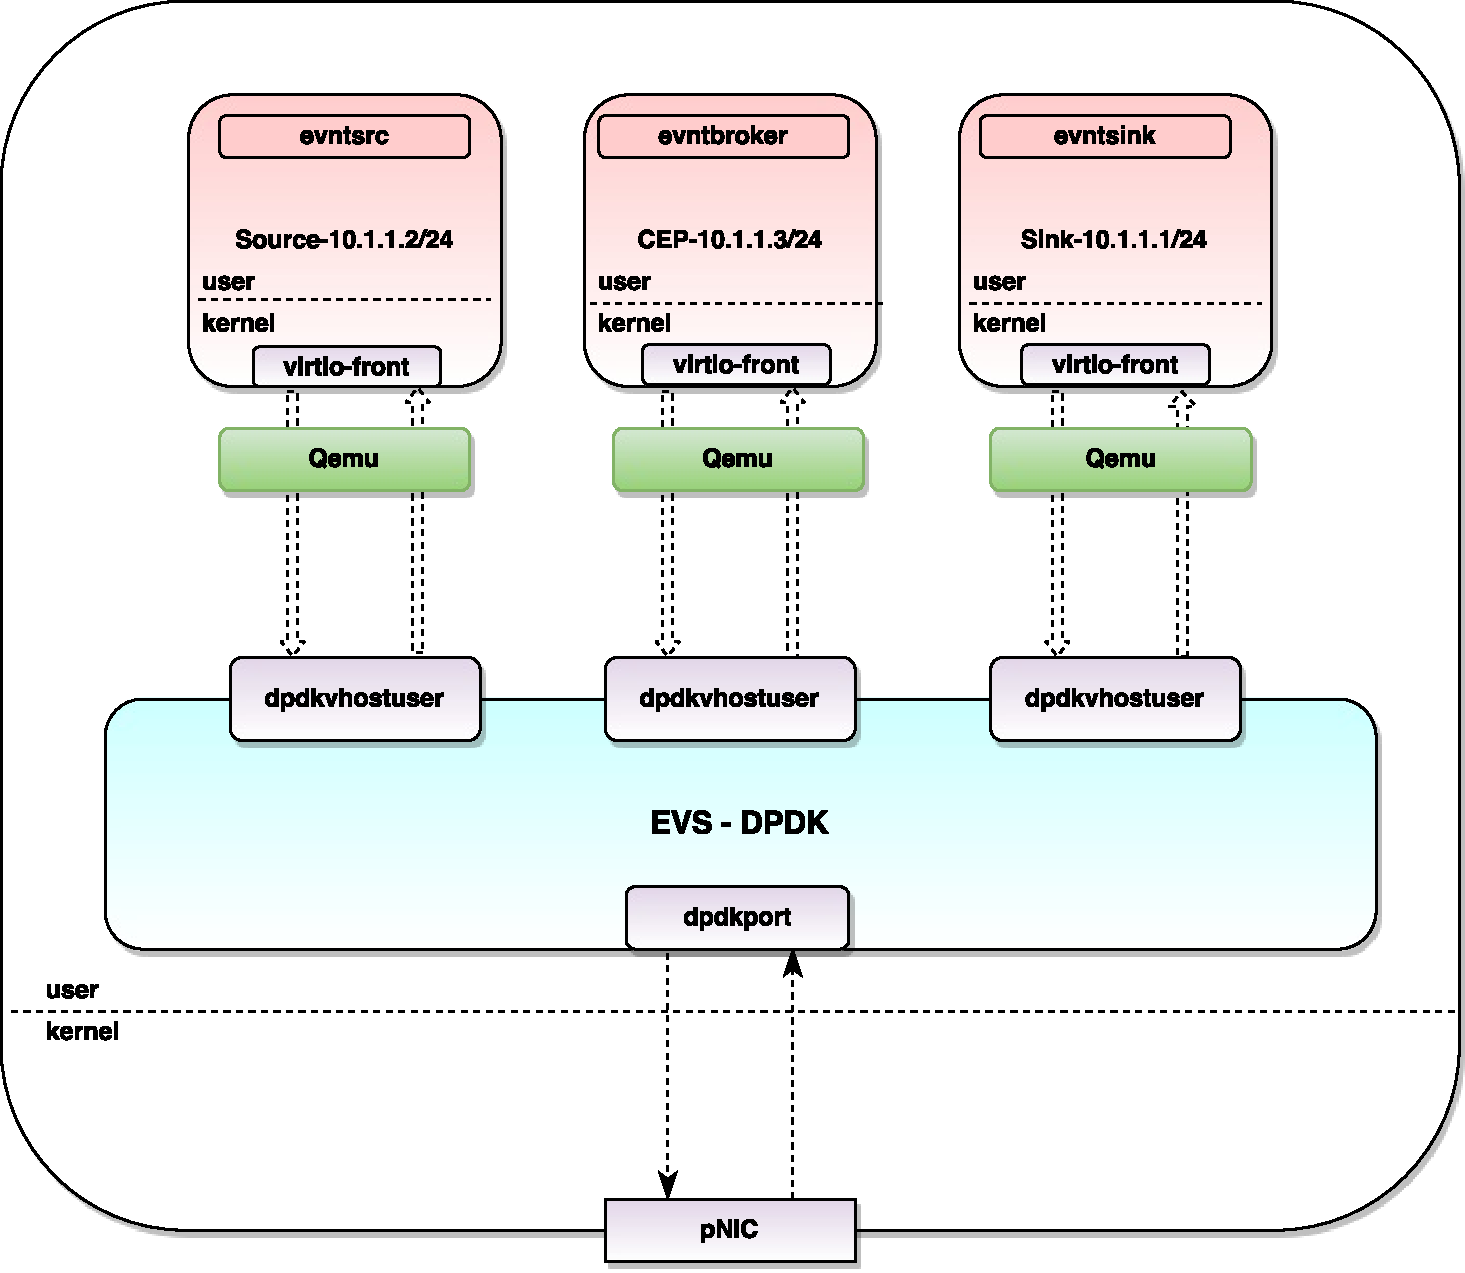
\includegraphics[height=12cm]{evsdpdk04.pdf}
\end{figure}


The set up is pictorially represented in Figure 5.16. More about the DPDK-vhost implementation is discussed in section 2.3.1. Evaluating on guest virtual machines has it's own challenges caused by clock drift. Although all the three VM's set up use the kvm_clock as the current clock source, when the system is tested with a data flow set up illustrated in Figure 5.1, the latency results are observed to be erratic. Each time the guests are restarted - which is necessary when changing from OVS to EVS - the observed latency between evntsrc and evntsink is different, sometimes even negative. This indicates that the guest's clocks are drifting despite the use of kvm_clock. Although Ubuntu specifically recommends that NTP servers shouldn't be set up within guests, the guests were set up with NTP servers to check for synchronization. However, the NTP servers in guests do not solve the issue of clock drift. Given this scenario, the Evaluation on Namespaces is done by measuring the round-trip latency of the events generated by the evntsrc application. The data flow set up for the evaluation is illustrated in Figure 5.17. In the case of the EVS-DPDK setup, the evntsrc application in KVM guest-1 sends the events to a counter and a timestamp to the evntsink on KVM guest-2 via the EVS bridge. The evntsink application receives the event and retransmits with the same event to the evntsrc again via the EVS bridge. The evntsrc application on receiving the response finds the delta between the timestamp in the event and the current timestamp to get the round-trip latency via the EVS bridge. This flow of data avoids the clock drift issue by ensuring that timestamps used to calculate the latency are generated within the same guest machine. In the case of OVS, an evntbroker application on KVM guest-3 acts as the broker for events.



 \begin{figure}[H]
 \centering
 \caption{Data Flow in EVS vs OVS DPDK}
 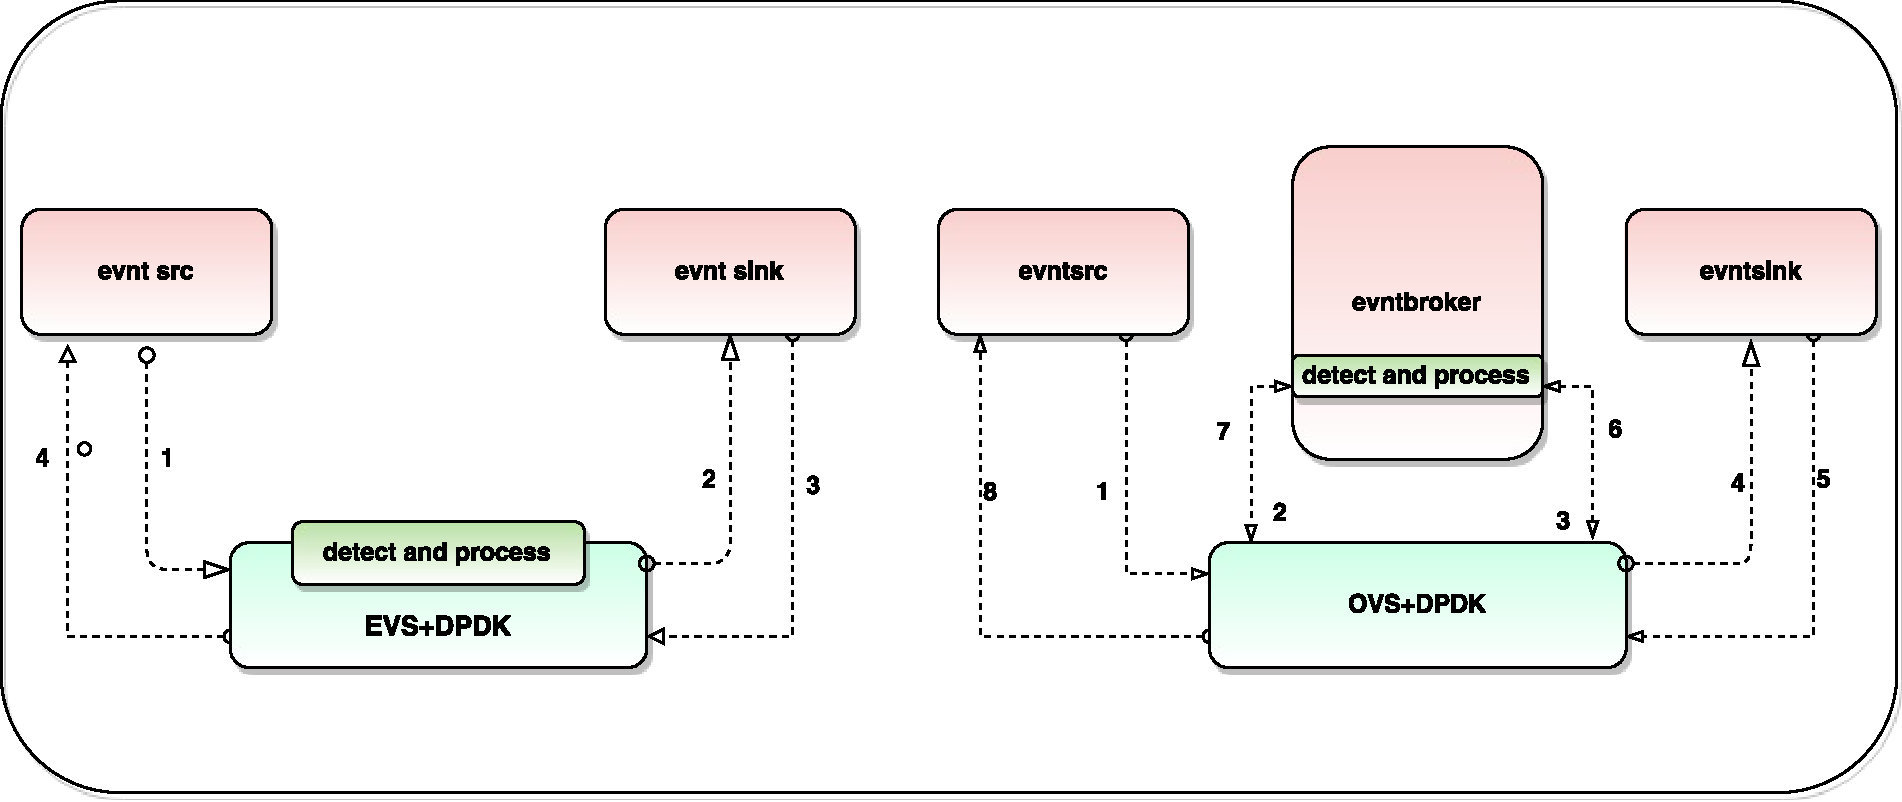
\includegraphics[height=7cm]{evsovsdpdk.pdf}
\end{figure}


The evaluation on KVM guests emulates a real-world data center deployment. The motivation for this evaluation is to repeat the evaluation done on network namespaces, but rather find insights to the questions that are left open after evaluation on network namespaces, namely:
\begin{itemize}
 \item The impact of the additional context-switch between the hypervisor and guests on latency. 
 \item The impact of high throughput on the compare operations which in current form rely on cache re-validation. 
\end{itemize}

\subsection{Guest-to-Guest Measurements}

Having established the key questions, the initial observations on guest-to-guest communication on the EVS bridge and OVS bridge regarding throughput, RTT, and average packet processing cycles per packet are detailed in Table 5.3. The EVS bridge introduces a three-fold increase in packet processing cycles per packet because of the additional processing needed to parse and de-serialize the events within the packet. But the burden is introduced only on tagged packets as is confirmed by the readings of per-packet processing on iperf3 packets on both the bridges shown. \newline \newline



\begin{center}
 \captionof{table}{OVS vs EVS DPDK comparision} \label{tab:title} 
 \begin{tabular}{ |c|c|c| }
  \hline
  \textbf{Parameter} &  \textbf{OVS Bridg}e &  \textbf{EVS Bridge} \\\toprule
  \hline
  Throughput  & 6.40 Gbps & 6.60 Gbps  \\
  \hline 
  hping3 RTT  & 4.0 ms & 4.9 ms \\
  \hline  
  Tagged packets - Avg processing 
  cycles per packet  &  6075.91 & 20472.32  \\ 
  \hline
  \hline  
  iperf3 - Avg processing 
  cycles per packet   &  2828.63 & 2811.79 \\\bottomrule  
 \end{tabular}
\end{center} 


\subsection{Performance measurement with event detection redirection - DPDK}
In this subsection, the performance evaluation of event detection and event redirection operation - 5.1 - is presented when performed on a hypervisor EVS-DPDK. This subsection is a counterpart of the evaluation performed on namespaces detailed in section 5.4.3. One key question left open by the evaluation on namespaces is whether the added context switch overhead that exists case of a hypervisor-guest deployment have an impact on the performance comparison of event detection and redirection operations performed on EVS against the same operations performed on a evntbroker in another guest. The flow of data for the evaluation is illustrated in Figure 5.20, and as described previously Round-trip latency is used instead of point-to-point latency. The event direction in the case of a virtualized L2 network is done using the mod_dl_dst action unlike the mod_nw_dst action in namespaces. A similar rule is installed to handle the redirection from 10.1.1.1 to 10.1.1.3.

\begin{lstlisting}[language=json,firstnumber=1]
{
"dpid": 178974088016461,
"table_id": 0,
"priority": 11112,
"flags": 1,
"match":{
"dl_type":0x0800,
"nw_proto":17,
"nw_src":"10.1.1.2",
"nw_dst":"10.1.1.3",
"tp_dst":9877,
"e_type":"TEMP",
},
"actions":[{
"type":"set_nw_dst",
"nw_dst": 10.1.1.1
},
{
"type":"set_dl_dst",
"dl_dst": 00:00:00:00:00:01
},
{
"type":"NORMAL"
}
]
}
http://localhost:8080/stats/flowentry/add \end{lstlisting}



\begin{figure}[H]
 \centering
 \caption{Performance of event redirection in bridged virtual machines}
 \begin{tikzpicture} [baseline=(current axis.outer east)]
 \begin{axis}[
 width=0.5\textwidth,
 xlabel={Trial},
 ylabel={Round Trip Latency(ms)},
 xmin=1, xmax=10,
 ymin=0.00, ymax=1.2,
 xtick={1,2,3,4,5,6,7,8,9,10},
 ytick={0.00,0.30,0.60,0.90,1.2},
 legend pos=north west,
 ymajorgrids=true,
 grid style=dashed,
 legend style={at={(0.5,1.15)},anchor=north}, legend columns=-1
 ]
 \addplot[
 color=red,
 mark=square,
 ]
 coordinates {
(1,0.73)
(2,0.52)
(3,0.47)
(4,0.52)
(5,0.42)
(6,0.26)
(7,0.47)
(8,0.57)
(9,0.421)
(10,0.36)

  
 };
 \addlegendentry{EVS - Avg 0.4741 ms}
 \addplot[
 color=green,
 mark=square,
 ]
 coordinates {
(1,0.526)
(2,0.473)
(3,0.526)
(4,0.473)
(5,0.473)
(6,0.473)
(7,0.789)
(8,0.421)
(9,0.526)
(10,0.421)
  
 };
 \addlegendentry{OVS - Avg 0.5101 ms}
 
 
 \end{axis}
 \end{tikzpicture}
\end{figure}



The results show that when event redirection is performed on EVS in a virtualization environment, removing the context switch from hypervisor to guest and back to hypervisor results in a lower round trip latency when compared to sending the events to the evntbroker for redirection. This is a key result which was not observed when the event redirection was performed in network namespaces. Avoiding the context switch - which exists in a data center/commodity server environment, does prove benifial in terms of avoiding latency and reducing network traffic. 

\subsection{Performance measure of compare operations and event redirection - DPDK}
In this subsection, the performance measure of compare operations and event redirection with bridged virtual machines on EVS DPDK is presented. The set up is similar to the set up in section 5.5.3, except for the rule installed. The operation in consideration is denoted as:

The operation supported by Greater than or equal to operator is denoted by:
\begin{equation}D(e.t  \wedge (e.a_1 <= value) \quad | \quad stream, \end{equation}
where \textit{D} is the detect operation; \newline
\textit{e.t} is the event type; \newline
\textit{e.a1} is the first event attribute; \newline
\textit{value} is the integer value to be compared with; \newline
| denotes the redirect operation; \newline
and \textit{stream} is the logical stream to which the detected event is redirected to. \newline \newline

The controller rule corresponding to this operation that is installed in EVS  is:

\begin{lstlisting}[language=json,firstnumber=1]
{
"dpid": 178974088016461,
"table_id": 0,
"priority": 11112,
"flags": 1,
"match":{
"dl_type":0x0800,
"nw_proto":17,
"nw_src":"10.1.1.1",
"nw_dst":"10.1.1.3",
"tp_dst":9877,
"e_type":"TEST",
},
"actions":[{
"type":"set_nw_dst",
"nw_dst": 10.1.1.2
},
{
"type":"set_dl_dst",
"dl_dst": 00:00:00:00:00:02
},
{
"type":"SET_MAX",
"val": 100
}
]
}
http://localhost:8080/stats/flowentry/add \end{lstlisting}

From the perspective of an event query language, the above rule can be expressed as:

\begin{verbatim}
INSERT INTO NEWTEMPSTREAM
SELECT * FROM TEMPSTREAM 
WHERE DEVICE_1.VALUE <=100
\end{verbatim}

\begin{figure}[H]
	\centering
	\caption{Performance of compare operation and event redirection in bridged virtual machines}
	\begin{tikzpicture} [baseline=(current axis.outer east)]
	\begin{axis}[
	width=0.5\textwidth,
	xlabel={Trial},
	ylabel={Round Trip Latency(ms)},
	xmin=1, xmax=10,
	ymin=0.00, ymax=1.2,
	xtick={1,2,3,4,5,6,7,8,9,10},
	ytick={0.00,0.30,0.60,0.90,1.2},
	legend pos=north west,
	ymajorgrids=true,
	grid style=dashed,
	legend style={at={(0.5,1.15)},anchor=north}, legend columns=-1
	]
	\addplot[
	color=red,
	mark=square,
	]
	coordinates {
		(1,0.36)
		(2,0.42)
		(3,0.57)
		(4,0.36)
		(5,0.47)
		(6,0.36)
		(7,0.63)
		(8,0.63)
		(9,0.42)
		(10,0.42)  
		
	};
	\addlegendentry{Guests on EVS - Avg 0.475 ms}
	\addplot[
	color=green,
	mark=square,
	]
	coordinates {
		(1,0.57)
		(2,0.68)
		(3,0.52)
		(4,0.473)
		(5,0.473)
		(6,0.63)
		(7,0.68)
		(8,0.73)
		(9,0.42)
		(10,0.47)
		
	};
	\addlegendentry{Guests on OVS - Avg 0.5646 ms}
	
	
	\end{axis}
	\end{tikzpicture}
\end{figure}

As plotted in the graphs in figure 5.19, for compare operations with disabled megaflow cache, the point-to-point latency in case of the EVS bridge model is slightly lower than while having an application broker in a standard OVS bridge. The results seen are similar to the plot in figure 5.18.


\subsection{Evaluating for accuracy of compare operations - DPDK}
In this subsection, the accuracy of the compare operations - 5.7 and 5.8 - is evaluated in a similar fashion detailed in 5.4.9. The aim of the evaluation is to see the impact of high bandwidth on the ideal rule hit rate for compare operations. Two approaches are considered for the evaluation: 
\begin{itemize}
 \item Disabled Megaflows
 \item Max-idle time - 1 ms
\end{itemize} 


\pgfplotstableread[row sep=\\,col sep=&]{
 Delay & Disabled & Max   \\
 7     & 94.73  & 49.2   \\
 8     & 95.68 & 65.3    \\
 9    & 96.65 & 88.32 \\
 10    & 96.2 & 96.73  \\
 11    & 96.12 & 96.76  \\
}\delaydata



\begin{figure}[H]
 \noindent\hrulefill
 
 \noindent
 \caption{Accuracy of  operations in EVS DPDK}
 \begin{tikzpicture}
 \begin{axis}[
 ybar,
 xlabel={Delay in Rule hit (ms)},
 ylabel={Accuracy of compare operations(percentage)},
 symbolic x coords={7,8,9,10,11},
 nodes near coords,
 legend style={at={(0.5,1)},
  anchor=south,legend columns=-1},
 ]
 \addplot[fill=green] table[x=Delay,y=Disabled]{\delaydata};
 \legend{Disabled Megaflow}
 \end{axis}
 \end{tikzpicture}
 \hfil
 \begin{tikzpicture}
 \begin{axis}[
 ybar,
 xlabel={Delay in Rule hit (ms)},
 ylabel={Accuracy of compare operations(percentage)},
 symbolic x coords={7,8,9,10,11},
 nodes near coords,
 legend style={at={(0.5,1)},
  anchor=south,legend columns=-1},
 ]
 \addplot[fill=red ] table[x=Delay,y=Max]{\delaydata};
 \legend{Max Idle Time 1ms}
 \end{axis}
 \end{tikzpicture}
\end{figure}


As plotted in the graph in figure 5.20, with disabled megaflows the EVS supports an accuracy of 94\% to 97\% when a flow rule is hit every 7ms, whereas with a configure idle time of 1 ms, an accuracy of 96\% is achieved only at a rule hit rate of 10 ms. This can be contrasted with the results in figure 5.11 and 5.12 where higher levels of accuracy were hit. To understand this difference more research work is proposed on the cache revalidation process in Open vSwitch. Future work may involve changing the re-validator to evict event processing rules at a higher rate compared to the other OpenFlow rules.


\subsection{Evaluation of processing cycles needed for event operations}
 The event processing pipeline in EVS is expensive in general, as shown in Table 5.3. Each tagged packet in this pipeline averages three times the average processing cycle. In this subsection, the evaluation of processing cycles needed for event operations is presented.
 
 
\begin{center}
 \captionof{table}{Processing cycles for event operations} \label{tab:title} 
 \begin{tabular}{ |c|c| }
  \hline
  \textbf{Parameter} &  \textbf{Average processing cycles per packet} \\\toprule
  \hline
  Tagged packets without detection  &  20472.9 \\
  \hline 
  Tagged packets with event type detection  & 20039.28 \\
  \hline  
  Tagged packets with event type and one attribute detection  &  20322.76  \\ 
  \hline
  Tagged packets with event type and two attributes detection  &  18623.9  \\ 
  \hline  
  Tagged packets with event type detection and redirection  &  31562.61  \\ 
  \hline  
  Tagged packets with compare operations with disabled megaflow   &  83275.34  \\\bottomrule  
 \end{tabular}
\end{center} 


The processing cycles needed per packet does not seem to vary as detection operations are performed on event attributes. However, when compare operations are performed with disabled megaflows, as they should be to reach an acceptable level of accuracy, the number of processing cycles needed nearly quadruple. This is because of the cache miss and additional OpenFlow pipeline look up per packet. Although an improvement in point-to-point latency is observed while performing compare operations on the EVS bridge, the significant increase in processing cycles per packet is a downside which demands improvement and further research.



	\chapter{Conclusion and Future Work}
In this chapter, the conclusions derived from the implementation and evaluation of the In-Network Event Processing framework are presented. The future work that can be undertaken to build up on the implementation and the conceivable improvements are additionally discussed. 




\section{Conclusion}
Network virtualization and software-defined networking offer boundless possibilities for provisioning chained network functions on demand with the aid of software-based solutions and programmable network control planes. As part of research conducted in the thesis, an exercise in programming the network control plane with application context and enabling the data plane to process application logic is presented within the context of a complex event processing ecosystem. To achieve the goals of the research the following contributions have been made:
\begin{itemize}
	\item An event processing framework is implemented within the highly adopted Open vSwitch.
	\item The vSwitch is enabled to perform logical and stateful operations based on user logic configured as event rules.
	\item A framework to remotely offload event rules onto the network control plane via HTTP is implemented using the RYU controller.
	\item A thorough evaluation of the implementation against several parameters is detailed and discussed.
\end{itemize}
The results of the evaluation demonstrate that the benefits of detecting and redirecting events at the vSwitch are compelling. In this model, the vSwitch assumes the role of an in-network broker. Evaluation of this model shows a reduction in point-to-point latency between the producers and consumers of events. By avoiding the utilization of and context switch to a broker application, a significant reduction in network traffic and processing is achieved for single staged systems. These results when extrapolated to multi-staged processing systems can potentially avoid multiple context switches and thereby improve the latency significantly, and reduce the burden on the network. However, the results also show an increased number of processing cycles per packet; which when weighed against the added benefits is a modest price to pay. When higher level logical and stateful operations are performed on event attributes, the benefits are less apparent in the current implementation. Although a reduction in network traffic, prevention of context switch to a broker and consequent avoidance of broker processing are observed, the number of processing cycles required per packet increases significantly because of reliance on the OpenFlow processing pipeline instead of the cache. In addition to the impact on the event processing pipeline, this also adversely impacts the generic performance of the Open vSwitch. A possible solution to this problem is presented in Section 6.1. Overall, the thesis elaborates on the potential of offloading aspects of event processing onto the underlying network. Although stateful event operations are implemented, the benefits are not apparent because of the current caching limitations. Nonetheless, while performing the role of an event broker, the benefits become more apparent. This provides network operators with promising avenues to explore models of complementing existing complex event processing ecosystems with highly tuned application-aware custom network solutions.

\section{Future Work}
In the current implementation, event processing actions do not take advantage of the megaflow cache implementation of the Open vSwitch. Instead, each event has to be looked up the OpenFlow processing pipeline and event actions have to be applied for accurate results. To achieve the same, the megaflow cache eviction rate is increased which results in poor performance of the Open vSwitch bridge. This is not ideal because it affects all the systems bridged using Open vSwitch and not just the implemented event processing pipeline. To avoid this problem, a sophisticated re-validator thread may be developed to evict only event based rules from the cache and allow other rules to remain cached. \newline
The implemented event processing within Open vSwitch results in a significant increase in processing cycles per packet. This is because, for each packet, the application layer is accessed, event attributes are extracted and deserialized for further processing. This adds significant cycles per packet. Future work may address this drawback to make the event extraction process much leaner than what it is currently.\newline
Furthermore, the current implementation focuses on the UDP transport protocol. Future work may extend the support to other protocols.
	%\chapter{Evaluation}
This chapter provides a description of the Evaluation test bed for the OpenVswitch-Event Processing System and a brief discussion of the results.

\section{Evaluation Testbed}
The system under test is the OpenVswitch userspace bridge. To set up the evaluation test bed, two network Namespaces are created and connected to the OpenVswitch bridge running in userspace mode. Namespace A runs a Java UDP event generator application, which is bridged via OpenVswitch - the system under test, to another Java application consuming the events in Namespace B, thereby simulating a Networked environment. The application at A timestamps the datagram before Send, for the application at B to compare the time stamp on Receive to get the point-to-point latency, which is aggregated over ${10^5}$ datagrams to get the latency.

\section{Parameters for Evaluation}
Two parameters are initially considered for the evaluation, namely, a) The measure of latency against rules with increasing size of event type field. b) The measure of latency against percentage of datagrams filtered on event type field.
\subsection{Size of Event Type}
As described in the system model, Event Type is a string field present in the first position of an event payload. The effects of performing a match on event type field with varying lengths to point-to-point latency is measured and the results are illustrated below in Figure 1.\newline
\begin{tikzpicture}
\begin{axis}[
title=Latency Measure with increasing size of Event Type,
ybar,
enlargelimits=0.15,
legend style={at={(0.5,-0.25)},
	anchor=north,legend columns=-1},
ylabel={Latency in milliseconds},
symbolic x coords={1,2,,3,4,5,6,7,8,9},
xtick=data,
nodes near coords,
nodes near coords align={vertical},
]
\addplot coordinates {(1,99.68)(2,99.69)(3,99.56)(4,94.64)(5,)(6,)(7,)(8,)(9,)};
%\addplot coordinates {(5,7.61)(10,7.79)(20,9.2)(40,25.05) };
%\addplot coordinates {(5,44.2)(10,63.2)(20,94.8)(40,118.3) };
%\legend{No. of flows,1ms delay,CPU LOAD}
\end{axis}
\end{tikzpicture}
 
The increasing size of event type string doesn't result in a linear increase in latency. This is explained by the fact that Tuple search space classifier of OpenVswitch creates a Hash table for every unique combination of inserted flow rule. In the case of this evaluation, one flow rule is added for each run, while increasing the size of event type field in consecutive runs. Additionally, although the event type field matches against a string in the event payload, the match field during flow rule insertion for event type is Hexadecimal value of the string. The rationale behind this approach is that strings within an event payload are serialized into Hexadecimal values on the wire, and since Event Parsing is part of the packet processing pipeline, keeping the fields as-is avoids the expensive conversion, thus reducing the overhead to the pipeline. So, to match an event payload with the an event type of 'A', the match field in the rule, 'e_type=0x41'

Figure 1 also contrasts the latency of an event type match with the latency measured for transport header match in OpenVswitch Master release 2.6.1 userspace bridge and a similar match on OpenVswitch-Event Processing(OVS-EP) bridge. The results show that the OVS-EP bridge adds a small latency even when the match levels are the same. This is because, the OVS-EP implementation has an Event Parsing layer part of the packet processing pipline and supports additional fields for matching on an Event Payload.

\subsection{Percentage of Flows Filtered}
Another interesting parameter that is evaluated is the rate of change of latency as increasing percentage of events are filtered. The results are illustrated in Figure 2.\newline
\newline
\newline
\newline
\newline
\newline\newline
Latency measure on Filtered Flow percentage
\newline
\newline
\newline
\newline\newline
\newline
\newline

 The important difference in the evaluation is that the event generator generates events for 10 different event types, and ten flow rules are added to explicitly forward these types. To begin the evaluation the flow rules for each type are modified to filter the event of those types only. So, we begin with ten flow rules with the NORMAL action and change the action to DROP as we progress through the evaluation. The results show that as flow rules are inserted to increase the percentage of filtered events, the latency remains steady. This is because the number of flow rules remain constant, only the actions on each flow rule is modified to increase filtered events. And since the Tuple Space Search Classifier only adds an additional Hashtable when there is an new combination of fields entered as a flow rule, even increasing the number flow rules, as long as they have the same match fields would not result in additional lookups.


	
	%======================================================
	% The back matter
	%======================================================
	%\cleardoublepage

	\refstepcounter{dummy}
	\addcontentsline{toc}{chapter}{\bibname}
	\bibliographystyle{alpha} % <--- layout of the bib
	\bibliography{Bibliography} % file name of your bib
	
	
\end{document}
%======================================================
%======================================================